%% LyX 2.3.2-2 created this file.  For more info, see http://www.lyx.org/.
%% Do not edit unless you really know what you are doing.
\documentclass[11pt,twoside]{iuphd}
\usepackage{amsmath}
\usepackage{amssymb}
\usepackage{fontspec}
\setmainfont[Mapping=tex-text]{Times New Roman}
\setcounter{secnumdepth}{3}
\setcounter{tocdepth}{3}
\usepackage{verbatim}
\usepackage{rotfloat}
\usepackage{booktabs}
\usepackage{mathrsfs}
\usepackage{enumitem}
\usepackage{pdfpages}
\usepackage{graphicx}
\usepackage{setspace}
\usepackage[all]{xy}

\makeatletter

%%%%%%%%%%%%%%%%%%%%%%%%%%%%%% LyX specific LaTeX commands.
\providecommand{\LyX}{L\kern-.1667em\lower.25em\hbox{Y}\kern-.125emX\@}
\let\@@LyX\LyX
\def\LyX{\@ensure@LTR{\@@LyX}}
%% Because html converters don't know tabularnewline
\providecommand{\tabularnewline}{\\}
%% A simple dot to overcome graphicx limitations
\newcommand{\lyxdot}{.}


%%%%%%%%%%%%%%%%%%%%%%%%%%%%%% Textclass specific LaTeX commands.
\newlength{\lyxlabelwidth}      % auxiliary length 
\providecommand*{\code}[1]{\texttt{#1}}

%%%%%%%%%%%%%%%%%%%%%%%%%%%%%% User specified LaTeX commands.
\usepackage{csquotes}
\usepackage{comment}
\usepackage{framed}
\usepackage{mathrsfs}
\usepackage{setspace}
\usepackage{dsfont}
\usepackage[AutoFallBack=true]{xeCJK}
\setCJKmainfont[FallBack=Batang]{SimSun}
% \usepackage{xeCJK}
% \setCJKmainfont{SimSun}

\usepackage[all]{xy}
\newcommand{\xyR}[1]{\xymatrixrowsep={#1}}
\newcommand{\xyC}[1]{\xymatrixcolsep={#1}}

%\usepackage[basic]{complexity}
\newcommand{\lang}[1]{{\ensuremath{\textsf{#1}}}}
\newcommand{\newlang}[2]{\newcommand{#1}{\lang{#2}}}
\newlang{\usat}{UNIQUE-SAT}
\newcommand{\ComplexityFont}[1]{%
{\ensuremath{\textsf{#1}}}%extra {} makes everyone happy.
}
\newcommand{\NP}{\ComplexityFont{NP}}

\usepackage{amsthm}
\theoremstyle{plain}
\newtheorem{prop}{Proposition}[chapter]
\newtheorem{thm}{Theorem}[chapter]
\newtheorem{lemma}{Lemma}[chapter]
\newtheorem{case}{Case}
\newtheorem{corollary}{Corollary}[chapter]

\theoremstyle{definition}
\newtheorem{definition}{Definition}[chapter]
\newtheorem{question}{Question}[chapter]
\newtheorem*{method}{Method}
\newtheorem{example}{Example}[chapter]
\newtheorem{postulate}{Postulate}[chapter]

\usepackage[braket,qm]{qcircuit}
\newcommand{\proj}[1]{\op{#1}{#1}}

\usepackage{unicode-math}
\RequirePackage{ifthen}
\@ifpackageloaded{unicode-math}{}{
 \newcommand{\symbf}{\mathbf}
 \newcommand{\symrm}{\mathrm}
 \newcommand{\symcal}{\mathcal}
 \newcommand{\symbb}{\mathbb}
}
\newcommand{\muB}{\ensuremath{\mu^{\symrm{B}}}}
\newcommand{\muC}{\ensuremath{\mu^{\symrm{C}}}}
\newcommand{\muF}{\ensuremath{\mu^{\symrm{F}}}}
\newcommand{\symrmL}{\ensuremath{\symrm{L}}}
\newcommand{\symrmR}{\ensuremath{\symrm{R}}}
\newcommand{\mul}[1][]{\ensuremath{\mu^{\symrmL{#1}}}}
\newcommand{\mur}[1][]{\ensuremath{\mu^{\symrmR{#1}}}}
\newcommand{\barmuD}{\ensuremath{\bar{\mu}^{\symrm{D}}}}
\newcommand{\events}{\ensuremath{\symcal{E}}}
\newcommand{\eventsC}{\ensuremath{\events_{\symrm{C}}}}
\newcommand{\set}[2]{\ensuremath{\left\{ {#1}\mathrel{}\middle|\mathrel{}{#2}\right\} }}
\newcommand{\gmult}{*}
\newcommand{\Fpx}[1]{\symbb{F}_{{#1}}}
\newcommand{\Fp}{\Fpx{p}}
\newcommand{\Fppx}[1]{\Fpx{{#1}^2}}
\newcommand{\Fpp}{\Fppx{p}}
\newcommand{\Fq}{\Fpx{q}}
\newcommand{\ff}[1]{\Fpx{#1}}
\newcommand{\ffzx}[2]{\Fpx{#1}^{{#2}\;*}}
\newcommand{\ffx}[2]{\Fpx{#1}^{{#2}}}
\newcommand{\ffzd}[1]{\ffzx{#1}{d}}
\newcommand{\ffd}[1]{\ffx{#1}{d}}
\newcommand{\VVec}[1]{\vec{\symbf{#1}}}
\newcommand{\mathReal}{\symbb{R}}
\newcommand{\mathComplex}{\symbb{C}}
\newcommand{\braket}[2]{\ip{#1}{#2}}
\newcommand{\todo}[1]{\textbf{TODO.~#1}}
\newcommand{\Eq}[1]{Eq.~(\ref{#1})}
\newcommand{\Sphere}[1]{\symbf{S}^{#1}}
\newcommand{\R}{\mathReal}
\newcommand{\rme}{\symrm{e}}
\newcommand{\rmi}{\symrm{i}}
\newcommand{\rmd}{\symrm{d}}
\newcommand{\CP}[1]{\mathComplex\symbf{P}^{#1}} % Complex projective space
\newcommand{\DCP}[1]{\symbf{D}\mathComplex\symbf{P}^{#1}} % Discrete complex projective
\def\fh{\mathfrak{h}}
\newcommand{\uf}{U_{\!f}}
\newcommand{\scalarPlus}{+}
\newcommand{\boolt}{\textsf{Bool}} 
\newcommand{\bfalse}{\texttt{\textbf{false}}}
\newcommand{\btrue}{\texttt{\textbf{true}}}
\newcommand{\dotprod}{dot product}
\newcommand{\Tr}{\ensuremath{\mathop{\mathrm{Tr}}\nolimits}}
\newcommand{\Psibar}{\overline{\Psi}}
\newcommand{\cardp}[2]{#1 \, \slash\!\! \slash \, #2}
\def\round{\mathop{\rm round}\nolimits}
\newcommand{\ps}{\texttt{+}}
\newcommand{\ms}{\texttt{-}}
\newcommand{\Hilb}{\symcal{H}}
\newcommand{\coreBorn}{\ensuremath{\overline{\Hilb}}}
\def\C{{\symbb{C}}}
\newcommand{\ultramodular}{\symcal{M}}
\newcommand{\ultramodularL}[1][]{\ensuremath{\ultramodular^{L{#1}}}}
\newcommand{\ultramodularR}[1][]{\ensuremath{\ultramodular^{R{#1}}}}
\newcommand{\frameL}[1][]{\ensuremath{f^{L{#1}}}}
\newcommand{\frameR}[1][]{\ensuremath{f^{R{#1}}}}
\newcommand{\pmeas}{\ensuremath{\mu}}
\newcommand{\nb}{\nolinebreak[3] }
\NewDocumentCommand{\jthSubsystem}{m O{} m}{{#1}_{#2}^{#3}}

\newcommand{\interval}[1]{{\normalfont\textsf{\textbf{#1}}}}
\newcommand{\imposs}{\interval{F}}
\newcommand{\necess}{\interval{T}}
\newcommand{\unknown}{\interval{U}}

\usepackage{xparse}
\NewDocumentCommand{\fnorm}{s m}{\mathsf{N}\IfBooleanT{#1}{^{-1}}\left({#2}\right)}

\usepackage{refcount}
% https://tex.stackexchange.com/questions/16866/how-can-i-use-footnotemark-with-a-ref-argument

\department{Department of Mathematics}
\department{Department of Computer Science}

\usepackage{datetime2}
\usepackage{datetime2-calc}
\monthGranted{\DTMmonthname{\month}}
\yearGranted{\the\year}

% https://wiki.lyx.org/LyX/Tables#tabularx
%% Hack by Heiko Oberdiek (on de.comp.text.tex)
\usepackage{tabularx}

%% Redefine the standard table
\let\ORIGtabular\tabular
\let\ORIGendtabular\endtabular
\let\ORIGtabularx\tabularx
\renewcommand*{\tabularx}{%
  \def\tabular{%
    \let\endtabular\ORIGendtabular
    \ORIGtabular
  }%
  \ORIGtabularx
}

\renewcommand{\tabularxcolumn}[1]{m{#1}}
\newcolumntype{Y}{>{\centering\doublespacing\arraybackslash}X}
\newcolumntype{M}[1]{>{\centering\doublespacing\arraybackslash}m{\widthof{#1}}}

% https://tex.stackexchange.com/questions/19094/allowing-line-break-at-in-inline-math-mode-breaks-citations/19100#19100
\AtBeginDocument{%
  \mathchardef\mathcomma\mathcode`\,
  \mathcode`\,="8000 
}
{\catcode`,=\active
  \gdef,{\mathcomma\nolinebreak[3]}
}

\usepackage[font=doublespacing]{caption}

\newcommand{\PhD}{Ph.D.\ }

\@ifundefined{showcaptionsetup}{}{%
 \PassOptionsToPackage{caption=false}{subfig}}
\usepackage{subfig}
\makeatother

\usepackage{polyglossia}
\setdefaultlanguage[variant=american]{english}
\setotherlanguage{arabic}
\setotherlanguage{bahasai}
\setotherlanguage{basque}
\setotherlanguage{french}
\setotherlanguage{german}
\setotherlanguage{italian}
\setotherlanguage{portuges}
\setotherlanguage{turkish}
\setotherlanguage{vietnamese}
\usepackage[style=numeric-comp,maxbibnames=10,doi=false,isbn=false,url=false]{biblatex}
\addbibresource{prop.bib}
\begin{document}
\title{Discrete Quantum Theories and Computing}
\author{Tai, Yu-Tsung}

\maketitle
%data for Acceptance Page
\committeeMember{Amr A. Sabry, \PhD} \committeeMember{Dylan
Paul Thurston, \PhD} \committeeMember{Gerardo Ortiz, \PhD} \committeeMember{Andrew
J. Hanson, \PhD} \committeeMember{Shouhong Wang, \PhD} \defensedate{November
29, 2018} \acceptancepage

%data for Copyright Page
\copyrightpage

\begin{dedication}To my parents, Cheng-Tien Tai (戴振沺) and Feng-Ming
Chang (張鳳鳴).\end{dedication}

\begin{comment}

\chapter*{Survey of the acknowledgments in theses}

I found the sentences in my Acknowledgments almost always contains
“thank” and looks boring. To improve my Acknowledgments, I briefly
read the Acknowledgments in other theses \cite{Chih2013,Sun2015,Lee2013,Chen2016,sabry1995formal}.
\end{comment}
\begin{acknowledgments*}
\begin{sidewaystable}
\begin{doublespace}
\noindent \centering{}\caption{\label{tab:committee}The professors served in all my committees.}
%% ERT block 1 (before LyX tabular)
\renewcommand{\tabular}{\tabularx{\linewidth}}
\renewcommand{\endtabular}{\endtabularx} 
\begin{tabular}{M{MATH-M781}M{Co-author}M{(\textarabic{عمرو~صبري})}M{Co-author}M{Thurston}M{Shouhong}M{Lawrence}Y}
\toprule 
Committee or course & Gerardo Ortiz & Amr\nolinebreak[3] A. Sabry\linebreak[3] (\textarabic{عمرو صبري}) & Andrew\nolinebreak[3] J. Hanson & Dylan\nolinebreak[3] Paul Thurston & Shouhong Wang\linebreak[3] (汪守宏) & Lawrence\nolinebreak[3] S.\linebreak[2] Moss & Relation with the dissertation\tabularnewline
\midrule
\midrule 
 & Co-author & Co-author & Co-author &  &  &  & Most of Chapters~\ref{chap:Conventional-Quantum-Theory}, \ref{chap:Unrestricted-Finite-Fields},
and~\ref{chap:DQT=000026DQC} is based on~\cite{geometry2013} and~\cite{DQT2014};
most of Chapter~\ref{chap:QIVPM} is based on~\cite{THOS2018}.\tabularnewline
\midrule 
Research committee & Co-chair & Co-chair & Member & Co-chair & Member &  & Some questions in the dissertation proposal are answered in Chapter~\ref{chap:QIVPM},
and some of the remaining ones are explained in Chapter~\ref{chap:Further-Discussion}.\tabularnewline
\midrule 
 &  & Supervisor &  &  &  &  & The application for \emph{Rethinking Foundations of Physics} 2017
workshop inspires Chapter~\ref{chap:Introduction}.\tabularnewline
\midrule 
Advisory committee & Member & Member & Member & Member &  &  & The survey of real computation in the Computer Science qualifying
exam (chaired by Prof.\ Sabry) inspires Chapter~\ref{chap:Introduction}.\tabularnewline
\midrule 
PHYS-P700 & Instructor &  &  &  &  &  & The textbook~\cite{Mermin2007} of \emph{Quantum Computation and Information}
is cited in Chapters~\ref{chap:Introduction}, \ref{chap:Conventional-Quantum-Theory},
\ref{chap:DQT=000026DQC}, and~\ref{chap:QIVPM}.\tabularnewline
\midrule 
CSCI-B629 &  & Instructor &  &  &  &  & The textbook~\cite{hottbook2013} of \emph{Homotopy Type Theory}
is cited in Sec.~\ref{discretequantumtheoryIIb}.\tabularnewline
\midrule
Tier 3 committee & Co-chair & Co-chair &  & Member &  & Co-chair & Two of the assigned papers \cite{Schumacher2012-SCHMQT,doi:10.1142/S0217984913500644}
in the Tier 3 exam~\cite{Mathematics2018} are cited in Chapters~\ref{chap:Introduction}
and~\ref{chap:Unrestricted-Finite-Fields}.\tabularnewline
\midrule
MATH-M781 &  &  &  &  &  & Instructor & The presented paper~\cite{Abramsky2012} of \emph{Coalgebra} is
cited in Sec.~\ref{subsec:Classical-and-Quantum}.\tabularnewline
\bottomrule
\end{tabular}% ERT block 2 (after LyX tabular)
\renewcommand{\tabular}{\ORIGtabular}
\renewcommand{\endtabular}{\ORIGendtabular} 
\end{doublespace}
\end{sidewaystable}
I want to thank the professors who served in all my committees. These
professors advised me as committee members and taught me while we
wrote papers together and when I took their courses. Most of my dissertation
is either based on these papers or inspired by the studies supervised
by them as listed in Table~\ref{tab:committee}. Especially, Prof.\ Andrew
J. Hanson, Prof.\ Gerardo Ortiz, and Prof.\ Amr A. Sabry\ (\textarabic{عمرو صبري})
meet me weekly for the past few years, read and tried to understand
what I typed which sometimes even myself cannot understand, taught
me how to organize them in ``English'' so that general audience
might be interested and have some chance to understand, and encouraged
me to participate seminars, workshops, and conferences. Prof.\ Lawrence
Moss invited me to present our results in the interdisciplinary logic
seminar and theory seminar in Computer Science and wrote an assessment
letter for me. Although not directly related to this dissertation,
the \textgerman[variant=german,spelling=new,babelshorthands=true]{Weil}
conjecture~\cite{hartshorne1977algebraic} on Grassmannians studied
with Prof.\ Dylan Paul Thurston and the quantum interpretation discussed
with Prof.\ Shouhong Wang (汪守宏) also broadened my understanding on
discrete and conventional quantum theories. I would like to express
my appreciation to all of these.

To have the current content of dissertation, I would also like to
thank John Gardiner for some inspiring discussion about quantum probability
measures over finite fields~\cite{Gardiner2014}. His research supervised
by Prof.\ Gerardo Ortiz inspired Sec.~\ref{subsec:Maximal-entanglement}
and~\ref{sec:Toward-IVPM}. Besides of my committee members, what
I learned from the teachers in other courses also helped me consolidate
this dissertation as listed in Table~\ref{tab:teacher}. Learning
other materials also made me more mature and easier to communicate
with others. I need to thank those who taught me, especially my English
teachers, Traci Nagle, Elizabeth ``Betsy'' Merceron, and Kexin ``Casey''
Chen (谌可心).

\begin{table}[!t]
\begin{doublespace}
\noindent \centering{}\caption{\label{tab:teacher}Other courses I took which is relevant to this
dissertation, where IUB stands for Indiana University Bloomington
and NTU stands for National Taiwan University.}
%% ERT block 1 (before LyX tabular)
\renewcommand{\tabular}{\tabularx{\linewidth}}
\renewcommand{\endtabular}{\endtabularx} 
\begin{tabular}{M{Chou~(周謀鴻)}cM{MATH-M522}Y}
\toprule 
Instructor & School & Course & Relation with the dissertation\tabularnewline
\midrule
\midrule 
Tom Lewis & IUB & SLST-T501 & Sec.~\ref{subsec:Discrete-Deutsch-algorithm} is based on the term
paper of \emph{Academic Writing}.\tabularnewline
\midrule 
Michael\nolinebreak[3] A. Mandell & IUB & MATH-M522 & The textbook~\cite{Hatcher2001} of \emph{Topology II} is cited
in Chapters~\ref{chap:Introduction} and~\ref{chap:Conventional-Quantum-Theory}.\tabularnewline
\midrule 
Steven Myers & IUB & CSCI-B502 & The textbook~\cite{AroraBarak2009} of \emph{Computational Complexity}
is cited in Sec.~\ref{modalquantumcomputing}.\tabularnewline
\midrule 
Valery Lunts & IUB & MATH-M501 & The textbook~\cite{DummitFoote2004} of \emph{Survey of Algebra}
is cited in Secs.~\ref{sec:background}, \ref{discretequantumtheoryI},
and~\ref{discretequantumtheoryIIb}.\tabularnewline
\midrule 
Huah Chu\linebreak[3] (朱樺\textenglish[variant=american]{)} & NTU & 221~U3830\linebreak[3] 221~U3840 & The textbook~\cite{Artin1991} of \emph{Algebra (I)} and \emph{(II)}
is cited in Secs.~\ref{subsec:Two-dimensional-Hilbert-Space}, \ref{subsec:Cyclic-Properties-of},
\ref{subsec:Complexified-Finite-Fields}, and~\ref{discretequantumtheoryIIb}.\tabularnewline
\midrule 
Jin-Tzu Chen\linebreak[3] (陳金次) & NTU & 201~31300 & The textbook~\cite{GAMELIN2003} of \emph{Functions of a Complex Variable}
is cited in Sec.~\ref{subsec:Vector-Spaces}.\tabularnewline
\midrule
Mo-Hong\linebreak[3] Chou (周謀鴻) & NTU & 221~U4290 & The textbook~\cite{GolubVanLoan1996} of \emph{Introduction to Computational Linear Algebra}
is cited in Sec.~\ref{subsec:Finite-Precision-Extension-of}.\tabularnewline
\bottomrule
\end{tabular}% ERT block 2 (after LyX tabular)
\renewcommand{\tabular}{\ORIGtabular}
\renewcommand{\endtabular}{\ORIGendtabular} 
\end{doublespace}
\end{table}
Many people have done everything to make my double-major smooth. I
need to thank all of their supports, financially or providing some
experience, as listed in my Curriculum Vitae at the end of the dissertation.
Most importantly, Prof.\ Amr A. Sabry\ (\textarabic{عمرو صبري})
helped me deal with the rules, supervised my reading courses for writing
our papers, and financially support me as a research assistant and
associate. In the department of Mathematics, I need to thank the directors
of graduate study in Mathematics, especially Prof.\ Christopher Judge,
Prof.\ Matthias Weber, and Prof.\ Michael A.\ Mandell; and the
graduate services assistant, Kate Forrest. In the department of Computer
Science, I want to thank the directors of \PhD study in Computer
Science, especially Prof.\ Yuqing Melanie Wu (吴愈青) and Prof.\ \textturkish{Funda
Ergun}; the graduate student office; the director of AI/UI assignments,
Charles Pope; and the infrastructure and technology group (ITG). Particularly,
I don't know how much computational power I consumed to count the
states in Sec.~\ref{subsec:Maximal-entanglement}. This computational
power not only came from the Linux systems in Computer Science but
also came from the Big Red II administrated by University Information
Technology Services (UITS). Indiana University Libraries was also
extremely helpful during my dissertation research. Except for a stack
of books I checked out directly, while the books are not in their
collection, I occasionally requested them via the Interlibrary Loan
service or recommended IU libraries to purchase them.

Except for the financial support via employment and award, I have
also supported by my family, especially my father Cheng-Tien Tai (戴振沺).
He always thinks one-step ahead and cares about my future more than
I do. Discussion with other family members and friends also helped
me to compose this dissertation, to do research, or to live better
in general, and I want to thank the following people which haven't
been listed previously:\footnote{For some of them, I only provide their Chinese names for two reason.
First, I might only know their Chinese names. Second, there are many
ways to translate a name to English, but I don't know which one they
choose.}

\begin{itemize}

\item The \PhD students in Mathematics, including Kin Wai Chan,
ChunHsien Lu (呂俊賢), Cong Zhou (周蔥), Junyan Xu (许俊彦), Zhipeng Lu (路志鹏),
Robert Rose, Neal Coleman, Dami Lee, Ruiyu Yang (杨瑞雨), Yingwei Li
(李盈伟), Yu-Yuan Chen (陳裕元), Jan-Li Lin (林展立), Ping Zhong, Chen Xu (徐晨),
Yiqiu Mao (茅一遒), Yu-Min Chung (鍾佑民), Shizhuo Zhang (张诗卓), Max Yining
Zhang (张忆宁), \textturkish{Ata Tuncer}, Hongming Nie (聂洪明), Sandeep
Bhupatiraju, Peng Wang, Guanglu Zhu (祝广路), Sailaja Gajula, Xuqiang
Qin (秦绪强), and \textvietnamese{Phuong Nguyen}, \ldots , etc.

\item Other members in Mathematics, including Weihua Liu (刘伟华),
Yinan ``Christina'' Wu (武怡楠), Cheng ``Freddie'' Shi (史程), Shabnam
Kavousian, and Tyler Bennett (班天瑞), \ldots , etc.

\item My officemates, especially, Inhak Hwang\ (황인학), Jiecao
Chen (陈洁操), Erfan Sadeqi~Azer, Chao ``Alan'' Tao (陶超), Haoyu Zhang
(张皓宇), Yadi Wei (魏雅廸), BoLi Fang (方博立), Yuan Xie (谢缘), and Mrinmoy
Maity, \ldots , etc.

\item My other friends having an office in Lindley or \textportuges{Luddy}
Hall, especially, Prof.~Daniel Leivant, Prof.~Paul Purdom, Prof.~Chung-Chieh
Shan (單中杰), Chao-Hong Chen (陳昭宏), Robert Rose, \textbasque{Bibrak
Chandio}, Yuxiang Jiang (蒋宇翔), Lei Wang (王磊), Diyue Bu (卜廸悦), Pei-Ying
Chen (陳珮瑩), Prof.~Qin Zhang (张勤), Praveen Narayanan, Liang Chen (陈亮),
\textfrench{Ambrose Bonnaire-Sergeant}, Ali Varamesh, Min-Chin Lin
(林旻瑾), and Career Services in the School of Informatics, Computing,
and Engineering, \ldots , etc.

\item My other family members, including my mother Feng-Ming Chang
(張鳳鳴), my grandmothers 戴許玉婷 and 張林枝, my sister Sih-Sian Tai (戴司嫻),
my cousins especially Caren Liu (劉鈺平) and Kiwi Liu (劉子綺), and my
aunts and uncles, \ldots , etc.

\item My roommates, including Meng-Wei Chen (陳孟瑋), Yu ``Larry''
Chen (陈煜), Kenshin Reita (禮田謙信), and Jing-Han Liou (劉經翰).

\item My classmates or friends in NTU, including Hao-Chun Lee (李浩君),
Hsien-Ching Kao (高憲慶), Wei Cheng (鄭維), Chin-Yi Lin (林金毅), Chun-Ting
Chen (陳俊廷), and Prof.~Chenying Huang (黃貞穎), \ldots , etc.

\item My friends living in the Tulip Tree Apartments, including Chao-Hong
Chen (陳昭宏), Tsaiyi Wu (吳采奕), Cheng ``Freddie'' Shi (史程), Ossama
Abdel~Gawwad, and Cathryn ``Cathy'' Creger-Chambers, \textbahasai{Sary
Silvhiany}, Shaozhuan Li (李绍颛), Chenwei Zhang (张晨薇), Shu-Nan ``Nancy''
Chang (張舒涵), and Ching-Chi ``Victoria'' Chang (張靖琪), \ldots , etc.

\item My AT\&T family plan members, especially Meng-Wei Chen (陳孟瑋),
Yao-yu Chih (池耀宇), and Xinyi ``Diana'' Gong (龚欣怡), \ldots , etc.

\item Other friends, including Shu-Ling Wang (王舒齡), Wan-Ling ``Wynnie''
Chang (張婉鈴), Yu-Jung Lin (林宇容), Winnie Lou (何慧芳), Yi-Rong Yang (楊宜蓉),
Yi-Chu Chang (張逸竹), Jim \textgerman[variant=german,spelling=new,babelshorthands=true]{Zimmerly},
Davis Chen (陳鵬舟), Zihang Shao (邵子航), Prof.~Ying Ding (丁颖), Hung-Chun
Chao (趙竑鈞), Guang Zuo (左光), Prof.~Jung-Chao Ban (班榮超), Prof.~Jyh-Chyi
Gong (龔治齊), 江靜宜, and the office of International Services\ldots ,
etc.

\end{itemize}

\noindent This list could be on and on and never ends. If you have
helped me in any form or provide any helpful information during my
\PhD study, but I forget to list you or your unit here. Please forgive
my bad memory.

Finally, I want to thank K9 Web Protection for blocking distractive
websites to keep me focus, and Jin-Ru Yang (楊謹如) for keeping the password
and helping me control myself in general.\end{acknowledgments*}

\begin{preface*}
\begin{itemize}
\item The latest PDF version of this thesis is in GitHub: \code{https://git.io/fxbuG}.
\item Its source code is typeset using \LyX{} \cite{LyX} in \code{https://git.io/fxbuE}
and the exported \LaTeX{} file is in \code{https://git.io/fhZBW}.
\item Any comments can be left in the Issue part of the GitHub repository:
\code{https://git.io/fxbug}.
\end{itemize}
Following explains how to compile the PDF from the \LaTeX{} source:
\begin{enumerate}
\item \label{enu:Clone-the-git}Clone the git repository of this thesis
\code{https://git.io/fhZP5} into your local directory and the thesis
document class \code{https://github.com/yuttai/iuphd} in a location
where the system can find.
\item In the local directory of this thesis, run \code{xelatex dissertation.tex}.
\item Run \code{biber dissertation}.
\item Run \code{xelatex dissertation.tex} several times until all the references
are resolved.
\end{enumerate}
The previous steps only tested in Microsoft Windows with MiK\TeX{}
2.9. Please report me if there is any difficulty to compile it. Besides,
to compile a PDF file from the \LyX{} source, just finish step~\ref{enu:Clone-the-git},
open \code{dissertation.lyx} in \LyX , and click the toolbar button

\includegraphics[width=1em]{buffer-view}.\end{preface*}

\begin{abstract*}Most quantum computing models are based on the continuum
of real numbers, while classical digital computers faithfully realize
only discrete computational models. Analog computers appear to be
an option, but in reality are far weaker than would be needed for
computational models requiring real numbers. One approach to resolving
this conflict is to find consistent mathematical ways to limit measurement
precision to computable contexts that do not require incomputable
real numbers. Our goal is to build more philosophically consistent
models by investigating discrete quantum computing using finite number
systems, and, alternatively, by incorporating finite precision measurement
using intervals into quantum theory.

We begin by replacing the continuum of complex numbers by discrete
finite fields in quantum theory. The simplest theory, defined over
unrestricted finite fields, is so weak that it cannot express Deutsch's
algorithm, but, paradoxically, is also so powerful that it can be
used to solve the $\usat$ problem, which is as hard as a general
$\NP$-complete problem.

Our second framework employs only finite fields over prime numbers
of the form $4\ell+3$, which possess no solutions to $x^{2}+1=0$,
and thus permit an elegant complex representation of the finite field
by adjoining $\rmi=\sqrt{-1}$. Because the states of a discrete $n$-qubit
system are in principle enumerable, we can count the number of states,
and determine the proportions of entangled and unentangled states.
Depending on how we model the measurement process, this improved framework
can be used to implement deterministic Deutsch's algorithm and the
probabilistic Grover search algorithm in a local region, but we still
haven't found a consistent way to treat quantum probability measures
in general.

Finally, we shift our attention to consider quantum interval-valued
probability measures (IVPMs), which potentially embody both finite
precision measurement and a sensible correspondence to standard quantum
probability. This interval-valued framework not only provides a natural
generalization of both classical IVPMs and conventional quantum probability
measures but also allows us to establish bounds on the validity of
the Kochen-Specker and Gleason theorems in realistic experimental
environments.\end{abstract*}

\tableofcontents{}

\chapter{Introduction\label{chap:Introduction}}

Since no human being can distinguish quantities differing only by
an arbitrarily small extent \cite{Turing_1937,Gisin2017}, we want
to incorporate this limitation into our quantum mechanical model to
better capture our ability to predict quantum phenomena and the power
of realistic quantum computers. Since we are agnostic about whether
the reality is ultimately discrete or continuous, we consider two
types of quantum models. By assuming the quantum states are ultimately
discrete and distinguishable, our first type of quantum theories replaces
the complex numbers by finite fields. We then focus on the limitation
of distinguishability itself, incorporate finite precision measurements
into our model, and consider quantum interval-valued probability measures.

After first suggested by Richard Feynman 40 years ago~\cite{Feynman1982Simulating},
IBM, \textitalian{Rigetti}, Google, Microsoft, and many other companies
and countries have started to build realistic quantum computers recently
\cite{Shieber2018,Kahn2019} seeking more efficient ways to simulate
chemical molecules and breaking RSA \cite{boneh1999twenty,wiki:RSAFactoring}.
No matter how to, classical or quantum, attack these two tasks, they
require two different types of quantities. On one hand, a question
and its answer of RSA are both discrete integers. On the other hand,
molecules are described by quantities including the domain of their
position wave functions and the probability amplitudes of these wave
functions, which look like continuous at first sight. However, either
these quantities might later be discovered to be discrete, or their
exact values may never be pinned down. Hence, modeling quantum computing
based on the exact values of continuous quantities cannot really describe
the computational power of a realistic quantum computer. To better
understand this issue without struggling with the quantum theory,
it is instructive to review how classical quantities are characterized
and computed.

Discrete quantities can be easily characterized by integers~\cite{ParkerBaldridge2004}.
Even if the proportion of integers are fractions, the operations among
fractions are essentially the same as those among integers over the
common denominator. In general, discrete computation can be reliably
repeated with exact equivalence, and any digital computer can faithfully
simulate a Turing machine limited only by the available memory and
time~\cite{Turing_1937}.

In contrast, the non-apparently discrete quantities confused many
cultures since the very beginning. For example, the ancient Chinese
philosopher Chuang-tzu (庄子) didn't believe these quantities have a
minimum unit and expressed ``If a one-foot-long stick is cut into
halves every day, the cutting will never come to an end''.\footnote{``一尺之棰,日取其半,萬世不竭。'' in Chinese \cite{Zhuangzi1999,Liu2018}.}
As another example, Greek mathematicians in the school of Pythagoras
believed every mathematical model must be ultimately discrete, and
they in legend murdered Hippasus because he proved there is no minimum
unit between a side of a square and its diagonal. Comparing the idea
that the length of a square's diagonal is not a physical quantity
or there is no square physically, working with a mathematical model
without minimum unit seems more appealing. Since the mathematical
models are continuous, their corresponding physical quantities are
naturally assumed to be continuous. Later, these continuous quantities
became the basic component of analog computers. After logarithms were
discovered, a slide rule, also known as a slipstick, was used to compute
multiplication, division, and more complex operations as a mechanical
analog computer~\cite{wiki:SlideRule}. Charge amplifiers are used
to build electrical analog computers and compute integration in calculus
\cite{wiki:Integrator,wiki:ChargeAmplifier}.

Although it is convenient to assume physical quantities are as continuous
as their mathematical models, each physical quantity discussed in
the previous paragraph could not have a simple one-to-one correspondence
with a real number. Chuang-tzu's stick is made by molecules and cannot
be cut in halves endlessly. The input charge of an integrator must
be an integer multiple of the elementary charge. A perfect square
cannot be drawn physically. Even we don't draw it, but merely ask
whether it exists in the space. This question is still beyond our
ability to answer because whether space itself is ultimately discrete
or continuous is still an unsolved question. Even if a perfect square
exists physically, we may not able to decide whether the ``square''
we discussed is really perfect or almost perfect differing only by
an arbitrarily small extent. Similar situation applying to the length
of a slide rule, it is beyond our ability to decide whether its length
is ultimately discrete or continuous. Even if its length is continuous,
identifying which real number represents its length requires infinite
precision, but the precision in reality is limited generally to three
or four significant figures~\cite{wiki:AnalogComputer}. As the results,
even if analog computers really store real numbers, they cannot be
precisely read, written, and used to branch the computation. The opposite
of the last statement is sometimes assumed by real computational models.
For example, Blum, Cucker, Shub, and Smale modeled their BCSS machine
to allow the operations of deciding whether a number is greater or
equal to zero over real numbers and whether a number is exactly zero
over complex numbers \cite{BSS1989,Ziegler2007,blum2012complexity}.
Hence, when the quantities used to branch the computation closes to
zero, the branch chosen by a BCSS machine cannot reliably predict
the branch chosen by a realistic analog computer. Since two branches
of computations may not have any relations, the follow-up computational
paths may be significantly different, and this difference is unlikely
to be compensated by error analysis techniques easily like the butterfly
effect. Therefore, we might not be able to utilize a realistic analog
computer to acquire the computational power predicted by this kind
of theoretical models.%
\begin{comment}
\todo{Maybe extended to consider probabilistic model? For BCSS machine,
maybe using the idea of BPP to define the complexity class is more
reasonable than P or NP?}
\end{comment}

\begin{sidewaystable}
\begin{doublespace}
\noindent \centering{}\caption{\label{tab:Comparison}Comparison between the classical quantities
and their mathematical models with the inspired quantum models.}
%% ERT block 1 (before LyX tabular)
\renewcommand{\tabular}{\tabularx{\linewidth}}
\renewcommand{\endtabular}{\endtabularx} 
\begin{tabular}{YcYY}
\toprule 
Physical quantity & Discrete & Discrete with extreme small units & Continuous, or no evidence to support they are discrete\tabularnewline
\midrule 
Computational device & Digital computer & Analog computer & Analog computer\tabularnewline
\midrule
\midrule 
Mathematical representation & Integer & Real number & Real number\tabularnewline
\midrule 
Computational model & Turing machine & BCSS machine & BCSS machine\tabularnewline
\midrule
\midrule 
How does the theoretical model predict the behavior of the physical
device? & Reliably & Not reliably, but after we have better technology to manipulate the
minimum units, we can more reliably predict the physical phenomenon
and their computational power by a better discrete model. & Not reliably, because precision can never be high enough, and the
difference between their computational power might not be able compensated
by error analysis techniques.\tabularnewline
\midrule 
Inspired quantum model &  & Quantum theories and computing over finite fields & Quantum interval-valued probability measures (QIVPM)\tabularnewline
\bottomrule
\end{tabular}% ERT block 2 (after LyX tabular)
\renewcommand{\tabular}{\ORIGtabular}
\renewcommand{\endtabular}{\ORIGendtabular} 
\end{doublespace}
\end{sidewaystable}
The situations for classical quantities and the computational power
above them are summarized in Table~\ref{tab:Comparison}, and two
possibilities for classical quantities inspires two types of quantum
models. Like its classical counterparts, quantum circuit model, the
most widely used model of quantum computing, manipulates quantities
which are not discrete apparently: the probability amplitudes of quantum
states, which are assumed in the field of complex numbers in the ``conventional
quantum theory'' (CQT).\footnote{Alternative terminology in the literature includes ``actual,'' ``standard,''
and ``ordinary'' quantum theory.} If the probability amplitudes are assumed to be ultimately discrete,
we choose to replace the field of complex numbers by discrete finite
fields for two reasons. On one hand, CQT is built upon the operations
among the probability amplitudes, and the probability amplitudes have
the required operations since the complex numbers form a field. On
the other hand, based on finite fields, we will define the fraction-like
cardinal probability which has extremely small units when the size
of the field is extremely large. Alternatively, even if the probability
amplitudes might never be found quantized, considering the precision
of quantities could still result in a better model. However, comparing
to the precision of probability amplitudes, it is easier to consider
the precision of their inducing probabilities because the idea of
``imprecise probability'' is well-studied classically \cite{Shafer1976,GilboaSchmeidler1994,Marinacci1999,JamisonLodwick2004,HuberRonchetti2009,Grabisch2016}.
\begin{comment}
\todo{Make sure whether realistic quantum computers could branch
their computation based on their probability amplitudes or measured
probabilities? If they can only branch on their measured probabilities,
it will provide another reason why we want to study the precision
of the inducing probabilities\ldots{} }
\end{comment}
This idea will be extended to quantum domain as quantum interval-valued
probability measure (QIVPM).

\begin{comment}
After a review of finite fields in Section~\ref{sec:background},
we proceed with a sequence of finite-field approaches that lead more
and more closely to the properties of conventional quantum computing.
\end{comment}
\begin{comment}
An $n$-qubit pure state in the conventional quantum theory (CQT)
is represented as a vector in the $2^{n}$-dimensional Hilbert space.
If we eliminate all symmetries, an irreducible state is actually a
point in the projective Hilbert space \cite{MosseriDandoloff2001,Jaeger2007}
also known as the complex projective space~$\CP{2^{n}-1}$ \cite{Hatcher2001,Bengtsson2007}.
These irreducible quantum states can also be classified as product
states and entangled states, and the latter one plays an essential
role for pure-state algorithms \cite{Mermin2007,Jaeger2007}.

Given a pure state~$\ket{\Phi}$, when we measure an observable represented
by a Hermitian matrix~$\mathbf{O}$, the measurement result is one
of the eigenvalues of $\mathbf{O}$. The probability of getting a
particular eigenvalue~$\lambda$ is $\melem{\Phi}{P}{\Phi}$, where
$P$ is the projection operator onto the eigenspace of $\lambda$.
This rule of computing the probability is called the Born rule \cite{Born1983,Mermin2007,Jaeger2007},
which is used when we want to extract information from a quantum computer.
For any mixed state~$\rho$, the generalized Born rule induces a
conventional quantum probability measure $\muB_{\rho}\colon\events\rightarrow[0,1]$,
where $\events$ is the set of all projection operators on a given
Hilbert space. Conversely, any quantum probability measure $\mu\colon\events\rightarrow[0,1]$
can be induced from a mixed state $\rho$ in the Hilbert space of
dimension $D\ge3$ according to Gleason's theorem \cite{gleason1957,Redhead1987-REDINA,peres1995quantum,RichmanBridges1999,Hamhalter2013}.
In other words, this state $\rho$ is the unique state consistent
with any given quantum probability measure.
\end{comment}
The geometrical structure of states in CQT is first reviewed in Sec.~\ref{CQC1qubitBloch.sec},
where a pure state is represented as a vector in a Hilbert space,
and an irreducible state is actually a point in a projective Hilbert
space \cite{MosseriDandoloff2001,Jaeger2007} also known as a complex
projective space \cite{Hatcher2001,Bengtsson2007}. In Sec.~\ref{sec:fuzzy},
we will construct a quantum probability space based on classical probability
spaces, apply Gleason's theorem \cite{gleason1957,Redhead1987-REDINA,peres1995quantum,RichmanBridges1999,Hamhalter2013}
to recover the Born rule \cite{Born1983,Mermin2007,Jaeger2007}, and
define the expectation value of an observable. The expectation value
will then be used in Sec.~\ref{sec:The-geometry-of} to define purity
which provides an easy entanglement test.

\begin{comment}
In Section~\ref{modalquantum}, we examine previously-introduced
quantum theories defined over unrestricted finite fields and show
in Section~\ref{modalquantumcomputing} that this approach leads
to theories with such bizarre powers that they are probably nonphysical.
Although a version of quantum theory defined over a two-valued field
can express simple algorithms such as quantum teleportation, it is
so weak that it cannot express Deutsch's algorithm. This quantum theory
is, however, also so powerful that it can be used to solve an unstructured
database search of size $N$ using $O(\log(N))$ steps, which outperforms
the known asymptotic bound $O(\sqrt{N})$ in conventional quantum
computing.
\end{comment}
\begin{comment}
Our first discrete model replaces the complex numbers with an unrestricted
finite field~$\mathbb{F}_{q}$ \cite{Schumacher2012-SCHMQT,DQT2014,SchumacherWestmoreland2010}.
In this model, an $n$-qubit state is a non-zero vector in $\mathbb{F}_{q}^{2^{n}}$.
When we measure a given state~$\ket{\Phi}$, an observable is replaced
by a basis~$\mathcal{B}$ of $\mathbb{F}_{q}^{2^{n}}$. Since $\ket{\Phi}$
can be represented by the summation across a unique subset~$\mathcal{S}$
of the basis~$\mathcal{B}$, whether it is possible or impossible
to measure a basis vector~$\ket{i}$ depends on whether $\ket{i}$
is in $\mathcal{S}$ or not. Because this model only predicts whether
a result is possible or impossible, it is called the modal quantum
theory. Its computational model, called the modal quantum computing,
is far from conventional quantum computing. Although modal quantum
computing can express simple algorithms such as quantum teleportation
\cite{BennettBrassardEtAl1993,peres1995quantum,Mermin2007,Jaeger2007},
it is so weak that it cannot express Deutsch's algorithm \cite{Deutsch1985,Mermin2007}.
This quantum theory is, however, also so powerful that it can be used
to solve an unstructured database search of size $N$ using $O(\log(N))$
steps, which outperforms the known asymptotic bound $O(\sqrt{N})$
in conventional quantum computing \cite{Grover:1996:FQM:237814.237866,BennettBernsteinBrassardVazirani1997,Mermin2007,Jaeger2007}.
\end{comment}
In Chapter~\ref{chap:Unrestricted-Finite-Fields}, we examine previously-introduced
quantum theories defined over unrestricted finite fields \cite{Schumacher2012-SCHMQT,DQT2014,SchumacherWestmoreland2010}.
It is called the modal quantum theory because it can only predict
whether a measurement result is possible or impossible, but not its
probability. Although a version of quantum theory defined over the
two-valued field can express simple algorithms such as quantum teleportation
\cite{BennettBrassardEtAl1993,peres1995quantum,Mermin2007,Jaeger2007,Schumacher2012-SCHMQT},
it is so weak that it cannot express Deutsch's algorithm \cite{Deutsch1985,Mermin2007,DQT2014}.
This quantum theory is, however, also so powerful that it can be used
to efficiently solve the $\usat$ problem~\cite{Papadimitriou1993},
which is as hard as a general $\NP$-complete problem~\cite{Valiant198685}.

\begin{comment}
Next, in Section \ref{discretequantumtheoryI}, we improve on this
by showing that for finite fields of order $p^{2}$, with the prime
$p$ of the form $4\ell+3$ ($\ell$ a non-negative integer), the
complex numbers have extremely compelling and natural discrete analogs
that permit a great many of the standard requirements of quantum computing
to be preserved. Under suitable conditions, we have amplitude-based
partitions of unity, unitary transformations, and entanglement, as
well as solutions to deterministic quantum algorithms such as the
algorithms of Deutsch, Simon, and Bernstein-Vazirani~\cite{NCbook,Mermin},
though still with some bothersome shortcomings. Because of the modular
nature of arithmetic in the finite complex field, it is not possible
to define an inner product in the usual sense, and we show in Section~\ref{discretequantumcomputingI}
that this leads to excessive computational power for the unstructured
database search problem for certain database sizes.
\end{comment}
\begin{comment}
Our second model called discrete quantum theory (I) considers only
finite fields of order $p^{2}$, with the prime $p$ of the form $4\ell+3$
($\ell$ a non-negative integer) \cite{geometry2013,DQT2014}. In
this model, an irreducible state is a vector in $\mathbb{F}_{p^{2}}^{2^{n}}$,
and can be reduced to a point in the discrete complex projective space~$\mathbb{DCP}^{2^{n}-1}$.
Among these irreducible states, the product states and entangled states
can not only be identified as in CQT but also be counted for different
$p$. Although the state space is a natural discrete analog to CQT,
this model still only predicts whether a measurement result is possible
or impossible, because it is not possible to define an inner product
in the usual sense due to the modular arithmetic~\cite{grove2002classical}.
Under suitable conditions, we can have deterministic quantum algorithms
such as the algorithms of Deutsch, Simon \cite{Simon:1994:PQC:1398518.1399019,Mermin2007,Jaeger2007},
and Bernstein-Vazirani \cite{Bernstein:1993:QCT:167088.167097,Mermin2007},
but this still leads to excessive computational power for the unstructured
database search problem for certain database sizes.
\end{comment}
In Sec.~\ref{discretequantumtheoryI} to~\ref{discretequantumcomputingI},
we improve on this by showing that for finite fields of order $p^{2}$,
$\Fpp$, with the prime $p$ of the form $4\ell+3$ ($\ell$ a non-negative
integer), the complex numbers then have extremely compelling and natural
discrete analogs that preserve a great many of the standard requirements
of quantum computing. In this model, the state of a discrete $D$-dimensional
system is a vector in the $D$-dimensional vector space over $\Fpp$
and can be reduced to a point in the discrete complex projective space.
Among these irreducible states, the product states and entangled states
could not only be identified as in CQT but also be counted for different
$p$. Despite the similarity between this model and CQT, it still
only predicts whether a measurement result is possible or impossible
because it is not possible to define an inner product in the usual
sense due to the modular arithmetic~\cite{grove2002classical}. Under
suitable conditions, we can have deterministic quantum algorithms
such as the algorithms of Deutsch, Simon \cite{Simon:1994:PQC:1398518.1399019,Mermin2007,Jaeger2007},
and Bernstein-Vazirani \cite{Bernstein:1993:QCT:167088.167097,Mermin2007},
but this still leads to excessive computational power for partially
solving the $\usat$ problem efficiently.

\begin{comment}
We are led, in Sections~\ref{discretequantumtheoryIIa} and~\ref{discretequantumtheoryIIb},
to develop a framework with further restrictions on~$p$ that \emph{locally\/}
recovers the structure and expected properties of conventional quantum
theory. Section~\ref{discretequantumtheoryIIa} locally recovers
the inner product space and Section~\ref{discretequantumtheoryIIb}
locally recovers a notion of probability. The development in both
sections exploits the fact that longer sequences of \textit{ordered\/}
numbers appear in the quadratic residues (numbers with square-roots
in the field) as the size of the field increases. Discrete quantum
computations whose calculations are confined to numbers in this ordered
sequence resemble conventional quantum computations. The size of the
field $p$ plays an important role in describing the resources needed
for the computation as larger problem sizes require a larger field
size to represent all intermediate numerical values. A significant
feature of our framework is that the resources needed for the measurement
process can be separated from the resources needed by the evolution
of the system being modeled. This interplay between the resources
used by the system under study and the resources used for the observation
process is a significant concept that is nonexistent in conventional
quantum computing and is exposed by our careful accounting of resources.

We note that the conventional mathematical framework based on the
real numbers allows one to distinguish states whose measurement outcomes
differ by infinitesimally small probabilities, e.g., $10^{-100}$
vs.~$0$. In the proposed framework of discrete quantum computing,
the finite size of the field implies a maximum precision for measurement:
a ``small'' field represents limited resources with which it becomes
impossible to distinguish states whose measurement outcomes differ
by an amount less than the resolution afforded by the field. It is
possible, however, to discriminate between such states at the cost
of moving to a larger field, i.e., by investing more resources in
the measurement process. We formalize this approach to measurement
using the novel notion of \textit{cardinal probability\/}, with numerical
labels corresponding to ``more probable, the same, or less probable,''
rather than a percentage-based likelihood measure. In cardinal probability,
relative outcomes are associated with intervals of ambiguity that
get smaller and more precise as the size of the field increases.

Finally, in Section~\ref{discretequantumcomputingII}, we apply our
discrete quantum theory to the study of two representative algorithms,
the deterministic Deutsch-Jozsa algorithm and the probabilistic Grover
algorithm~\cite{NCbook,Mermin}. The first algorithm highlights the
role played by the size of the field $p$ in determining the actual
resources required for computation as the number of input bits $n$
increases, a concept nonexistent in conventional quantum computing.
The second algorithm highlights, in addition, the dependence of the
precision of measurement (via cardinal probabilities) on the size
of the field, another nonexistent concept in conventional quantum
computing.
\end{comment}
\begin{comment}
Our third model, discrete quantum theory (II)~\cite{DQT2014}, restricts
states in some local region of $\mathbb{F}_{p^{2}}^{2^{n}}$. Within
a local region, a notion of inner product and probability could be
recovered. Its discrete quantum computing can be further applied to
the deterministic Deutsch-Jozsa algorithm \cite{DeutschJozsa1992,Jaeger2007}
and the probabilistic Grover algorithm \cite{Grover:1996:FQM:237814.237866,Mermin2007,Jaeger2007}.
\end{comment}
Since many important quantum algorithms are probabilistic, we want
to find a notion of probability for quantum theories over finite fields.
The cardinal probability defined in Sec.~\ref{sec:Discrete-Quantum-Theory-(II)}
restricts states in some local regions of the vector spaces, where
a notion of inner product and probability could be recovered. In Sec.~\ref{discretequantumcomputingII},
this discrete quantum theory is applied to two representative algorithms,
the deterministic Deutsch-Jozsa algorithm \cite{DeutschJozsa1992,Jaeger2007}
and the probabilistic Grover algorithm \cite{Grover:1996:FQM:237814.237866,Mermin2007,Jaeger2007}.
\begin{comment}
When people tried to define quantum probability over finite fields,
people tended to treat the original Born rule as an axiom and tried
to modify it to get a discrete Born rule \cite{Schumacher2012-SCHMQT,doi:10.1142/S0217984913500644,DQT2014,Ellerman2016a}.
However, any modified Born rule could hardly work on the whole vector
space, since there is no inner product on the whole vector space over
finite fields. Instead of treating the Born rule as an axiom, the
Born rule can be deduced from a set of abstract definitions and axioms
according to Gleason's theorem. Although we might hope to deduce a
discrete Born rule directly from a similar set of definitions and
axioms, no discrete Born rule satisfies certain properties motivated
by Gleason's theorem with infinitely precise real-number probability~\cite{Gardiner2014}.
Since the state spaces are now discrete and finite, this suggests
us to consider a discrete Born rule mapping to a finite number of
intervals called interval-valued probability~\cite{JamisonLodwick2004,THOS2017}.
To adopting the idea of interval-valued probability step-by-step,
before attempting to study quantum interval-valued probability over
finite fields, we will first review the classical interval-valued
probability and extend it with the conventional quantum theory.
\end{comment}
Despite the great success of cardinal probabilities, it is difficult
to define their arithmetic operations and expectation values. Since
they could be defined easily with real-valued probabilities in CQT,
we attempt to consider real-valued quantum probability measures over
finite fields (QPMFF) in Sec.~\ref{sec:Toward-IVPM}. In contrast
to CQT, our Gleason-like conditions over finite fields cannot deduce
a discrete Born rule in general. This impossible result suggests that
the discrete and finite state spaces might not be compatible with
infinitely precise real-valued probability. Thus, no matter whether
the probability amplitudes are ultimately discrete or continuous,
we should study imprecise quantum probabilities formulated by quantum
interval-valued probability measures.

\begin{comment}
In the classical setting, there are several proposals for ``imprecise
probabilities'' \cite{Shafer1976,GilboaSchmeidler1994,Marinacci1999,JamisonLodwick2004,HuberRonchetti2009,Grabisch2016}.
Although these proposals differ in some details, they all share the
fact that the probability $\bar{\mu}(E)$ of an event~$E$ is generalized
from a single \emph{real number} to an \emph{interval}~$[l,r]$,
where~$l$ intuitively corresponds to the strength of evidence for
the event~$E$ and~$1-r$ corresponds to the strength of the evidence
against the same event. Given a sample space~$\Omega$ and a set
of intervals~$\mathscr{I}$, like a classical probability measure
$\mu\colon2^{\Omega}\rightarrow\left[0,1\right]$, a classical interval-valued
probability measure (IVPM) $\bar{\mu}\colon2^{\Omega}\rightarrow\mathscr{I}$
needs to satisfy some coherent axioms. By satisfying the convexity
axiom \cite{Shapley1971,GilboaSchmeidler1994,Marinacci1999,Grabisch2016},
Shapley proved that there is always a classical probability measure
consistent with the classical IVPM~$\bar{\mu}$ \cite{Shapley1971,GilboaSchmeidler1994,Grabisch2016}.
Given any random variable, its expectation value with respect to classical
probability measures consistent with~$\bar{\mu}$ is consistent with
its Choquet integral \cite{Choquet1954,GilboaSchmeidler1994,Grabisch2016}
with respect to $\bar{\mu}$ \cite{Rosenmuller1971,GilboaSchmeidler1994,Grabisch2016}.

The quantum extension, quantum interval-valued probability measure
(QIVPM) $\bar{\mu}\colon\events\rightarrow\mathscr{I}$, is a generalization
of both classical IVPMs $\bar{\mu}\colon2^{\Omega}\rightarrow\mathscr{I}$
and conventional quantum probability measures $\mu\colon\events\rightarrow[0,1]$
\cite{THOS2017}, because QIVPMs reduce to classical IVPMs when the
space of quantum events $\events$ is restricted to mutually commuting
events and reduce to conventional quantum probability measures when
mapping to infinitely precise uncountable intervals $\mathscr{I}_{\infty}=\set{\left[x,x\right]}{x\in\left[0,1\right]}$.
While Shapley and Gleason both proved there must be a ``state''
consistent with any given QIVPM in the reduced cases, in general,
there exists a QIVPM such that no state is consistent with it. However,
we found a class of QIVPMs such that all QIVPMs in this class are
consistent with a non-empty ``ball'' of quantum states whose radius
is defined by the maximal length of the intervals and recovers the
original Gleason theorem asymptotically. Similarly, the conventional
quantum expectation value and the classical Choquet integral are together
generalized to the quantum interval-valued expectation value. This
is used to prove an imprecise Kochen-Specker theorem \cite{BELL_1966,kochenspecker1967,Redhead1987-REDINA,peres1995quantum,Jaeger2007}
which suggests a possible resolution of the Meyer-Mermin debate on
the impact of finite-precision measurement on the Kochen-Specker theorem
\cite{PhysRevLett.83.3751,Mermin1999}.
\end{comment}
\begin{comment}
We present a mathematical framework based on quantum interval-valued
probability measures to study the effect of experimental imperfections
and finite precision measurements on defining aspects of quantum mechanics
such as contextuality and the Born rule. While foundational results
such as the Kochen-Specker and Gleason theorems are valid in the context
of infinite precision, they fail to hold in general in a world with
limited resources. Here we employ an interval-valued framework to
establish bounds on the validity of those theorems in realistic experimental
environments. In this way, not only can we quantify the idea of finite-precision
measurement within our theory, but we can also suggest a possible
resolution of the Meyer-Mermin debate on the impact of finite-precision
measurement on the Kochen-Specker theorem.
\end{comment}
Sec.~\ref{sec:Interval-Uncertainty} starts from reviewing how to
formulate classical ``imprecise probabilities'' \cite{Shafer1976,GilboaSchmeidler1994,Marinacci1999,JamisonLodwick2004,HuberRonchetti2009,Grabisch2016}
as interval-valued probability measures (IVPMs). Given a classical
IVPM, its core is the set of the real-valued probability measures
consistent with it \cite{Shapley1971,GilboaSchmeidler1994,NgMoYeh1997Chinese,Grabisch2016},
and the expectation value with respect to it is just classical Choquet
integral \cite{Choquet1954,GilboaSchmeidler1994,Grabisch2016}. These
classical properties can naturally be extended for QIVPMs when we
extend classical IVPMs to QIVPMs. In Sec.~\ref{sec:Kochen-Specker},
we utilize the expectation values while proving the finite precision
variants of the Kochen-Specker theorem \cite{BELL_1966,kochenspecker1967,Redhead1987-REDINA,peres1995quantum,Jaeger2007},
and establish bounds on its validity in realistic experimental environments.
In Sec.~\ref{sec:Gleason}, we are able to show that, while a QIVPM
incorporating the effects of finite precision might not be consistent
with Gleason's unique state~$\rho$ on all projectors defined on
a Hilbert space~$\Hilb$ of dimension $D\ge3$, it is possible to
construct a class of QIVPMs representing bounded resources that is
parameterized by the size of the intervals, and the original Gleason
theorem could be recovered for this class of QIVPMs asymptotically.

\begin{sidewaystable}
\begin{doublespace}
\noindent \centering{}\caption{\label{tab:organization}Comparison among our models, where the upper
half of the table lists their quantum mechanical definitions and properties,
and the lower half of the table lists their computational power.}
%% ERT block 1 (before LyX tabular)
\renewcommand{\tabular}{\tabularx{\linewidth}}
\renewcommand{\endtabular}{\endtabularx} 
\begin{tabular}{YYYYYYY}
\toprule 
 & Conventional & Modal & Discrete (I) & Discrete (II) & QPMFF & QIVPM\tabularnewline
\midrule
\midrule 
 & Chapter~\ref{chap:Conventional-Quantum-Theory} & Sec.~\ref{modalquantum} & Sec.~\ref{discretequantumtheoryI} to \ref{sec:Geometry-of-Entangled-States} & Sec.~\ref{sec:Discrete-Quantum-Theory-(II)} & Sec.~\ref{sec:Toward-IVPM} & Chapter~\ref{chap:QIVPM}\tabularnewline
\midrule 
States space & $\mathbb{C}^{D}$ & $\Fq^{D}$ & $\Fpp^{D}$ & Local region in~$\Fpp^{D}$ & $\Fpp^{D}$ & $\mathbb{C}^{D}$\tabularnewline
\midrule 
Likelihood of events is predicted by & Real-valued probability & Possible or impossible & Possible or impossible & Cardinal probability & Real-valued probability, but no sensible Born rule & Interval-valued probability\tabularnewline
\midrule 
Expectation value & Defined & Undefined & Formally defined & Undefined &  & Defined\tabularnewline
\midrule
\midrule 
 &  & Sec.~\ref{modalquantumcomputing} & Sec.~\ref{discretequantumcomputingI} & Sec.~\ref{discretequantumcomputingII} &  & \tabularnewline
\midrule 
Deutsch's algorithm & Yes & Maybe no & Yes & Yes &  & \tabularnewline
\midrule 
Efficiently solve $\usat$ & Unlikely & Yes & Partially & Unlikely &  & \tabularnewline
\midrule 
Grover search algorithm & Yes &  &  & Yes &  & \tabularnewline
\bottomrule
\end{tabular}% ERT block 2 (after LyX tabular)
\renewcommand{\tabular}{\ORIGtabular}
\renewcommand{\endtabular}{\ORIGendtabular} 
\end{doublespace}
\end{sidewaystable}
The organization of this thesis is summarized in Table~\ref{tab:organization},
and finally, Chapter~\ref{chap:Further-Discussion} contains further
extended questions, especially, briefly explaining why it might be
hard to recover Gleason's theorem for general QIVPMs.


\chapter{Conventional Quantum Theory\label{chap:Conventional-Quantum-Theory}}

The part of conventional quantum theory (CQT) used by the quantum
circuit model is described by the following:
\begin{enumerate}[label=(\roman{enumi})]
\item \label{enu:-orthonormal-basis}$D$ orthonormal basis vectors for
a Hilbert space of dimension~$D$,
\item \label{enu:probability-amplitude}$D$ complex probability amplitude
coefficients describing the contribution of each basis vector,
\item \label{enu:unitary-matrix}a set of probability-conserving unitary
matrix operators that suffice to describe all required state transformations
of a quantum circuit,
\item \label{enu:measurement-framework}and a measurement framework.
\end{enumerate}
In Sec.~\ref{CQC1qubitBloch.sec}, we focus on the geometric issues
raised by the properties~\ref{enu:-orthonormal-basis} and~\ref{enu:probability-amplitude}
given above for CQT\@. In Sec.~\ref{sec:fuzzy}, we introduce the
important issues of~\ref{enu:measurement-framework} and the foundations
of quantum probability space. The expectation values defined in Sec.~\ref{sec:fuzzy}
will be used to understand the geometry of entangled states in Sec.~\ref{sec:The-geometry-of}.
The property~\ref{enu:unitary-matrix} directly related to quantum
circuits will be introduced later in Chapters~\ref{chap:Unrestricted-Finite-Fields}
and~\ref{chap:DQT=000026DQC} when we dive into quantum algorithms.

\section{Geometrical Structure of States\label{CQC1qubitBloch.sec}}

There are many things that are assumed in CQT, such as the absence
of zero norm states for non-zero vectors, and the decomposition of
complex amplitudes into a pair of ordinary real numbers. One also
typically assumes the existence of a $D$-dimensional Hilbert space
with an orthonormal basis, allowing us to write \textit{pure} states
in general as Hilbert space vectors with a Hermitian inner product:
\begin{equation}
\ket{\Psi}=\sum_{i=0}^{D-1}\alpha_{i}\ket{i}\,.
\end{equation}
Here $\alpha_{i}\in\mathComplex$ are complex probability amplitudes,
$\VVec{\alpha}\in\mathComplex^{D}$, and the $\{\ket{i}\}$ is an
orthonormal basis of states obeying $\braket{i}{k}=\delta_{ik}$.

The meaning of this is that any state $\ket{\Phi}=\sum_{i=0}^{D-1}\beta_{i}\ket{i}$
can be projected onto another state $\ket{\Psi}$ by writing 
\begin{equation}
\braket{\Phi}{\Psi}=\sum_{i=0}^{D-1}\beta_{i}^{*}\alpha_{i}\,,
\end{equation}
thus quantifying the proximity of the two states. (Here $^{*}$ denotes
complex conjugation.) This is one of many properties we take for granted
in continuum quantum mechanics that challenge us in defining a discrete
quantum geometry. To facilitate the transition to DQT carried out
in later sections, we concern ourselves first with the properties
of the simplest possible abstract state object in CQT, the single
qubit state.

\subsection{Two-dimensional Hilbert Space\label{subsec:Two-dimensional-Hilbert-Space}}

A state in a two-dimensional Hilbert space, known as a qubit, already
provides access to a wealth of geometric information and context.
When we write the single qubit state as $\ket{\psi_{1}}=\alpha_{0}\ket{0}+\alpha_{1}\ket{1}$,
a convenience for computing probability and relative state properties
is the normalization condition 
\begin{equation}
\left\Vert \psi_{1}\right\Vert ^{2}=\left|\alpha_{0}\right|^{2}+\left|\alpha_{1}\right|^{2}=\alpha_{0}^{*}\alpha_{0}+\alpha_{1}^{*}\alpha_{1}=1\,,\label{A2.eq}
\end{equation}
which identifies $\alpha_{0}$ and $\alpha_{1}\in\mathbb{C}$ as probability
amplitudes and implies the conservation of probability in the closed
world spanned by $\left\{ \ket{0},\ket{1}\right\} $. Note that we
distinguish for future use the \textit{norm}~$\left\Vert \cdot\right\Vert $
of a vector from the \textit{modulus}~$\left|\cdot\right|$ of a
complex number. Continuing, we see that if we want only the irreducible
state descriptions, we must supplement the process of computing \Eq{A2.eq}
by finding a way to remove the distinction between states that differ
only by an overall phase transformation $\rme^{\rmi\theta}$, that
is, $\alpha_{0}\ket{0}+\alpha_{1}\ket{1}$ and $\rme^{\rmi\theta}\alpha_{0}\ket{0}+\rme^{\rmi\theta}\alpha_{1}\ket{1}$
are representing the same physical state. This can be accomplished
by the Hopf fibration \cite{Artin1991,Hatcher2001,MosseriDandoloff2001,Hanson2006,Bengtsson2007,wiki:HopfFibration},
which can be written down as follows: let $\alpha_{0}=x_{0}+\rmi y_{0}$
and $\alpha_{1}=x_{1}+\rmi y_{1}$. Then \Eq{A2.eq} becomes the
condition that the four real variables describing a qubit denote a
point on the three-sphere $\Sphere{3}$ (a 3-manifold) embedded in
$\R^{4}$: 
\begin{equation}
{x_{0}}^{2}+{y_{0}}^{2}+{x_{1}}^{2}+{y_{1}}^{2}=1\,.\label{A5.eq}
\end{equation}

\begin{figure}[!b]
\hfill{}\subfloat[]{\centering{}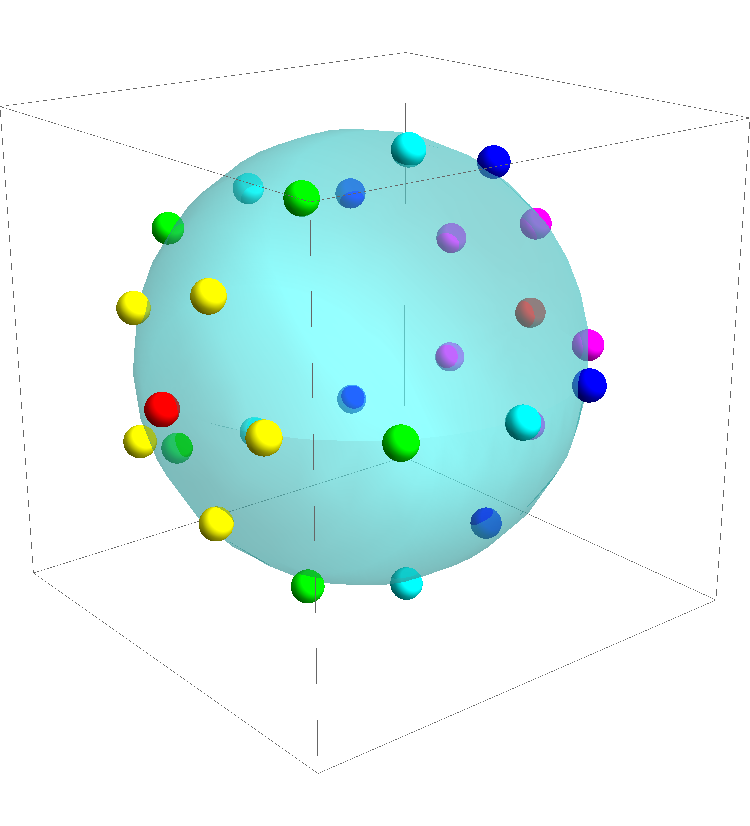
\includegraphics[width=0.48\columnwidth]{hopfS2}}\hfill{}\subfloat[]{\begin{centering}
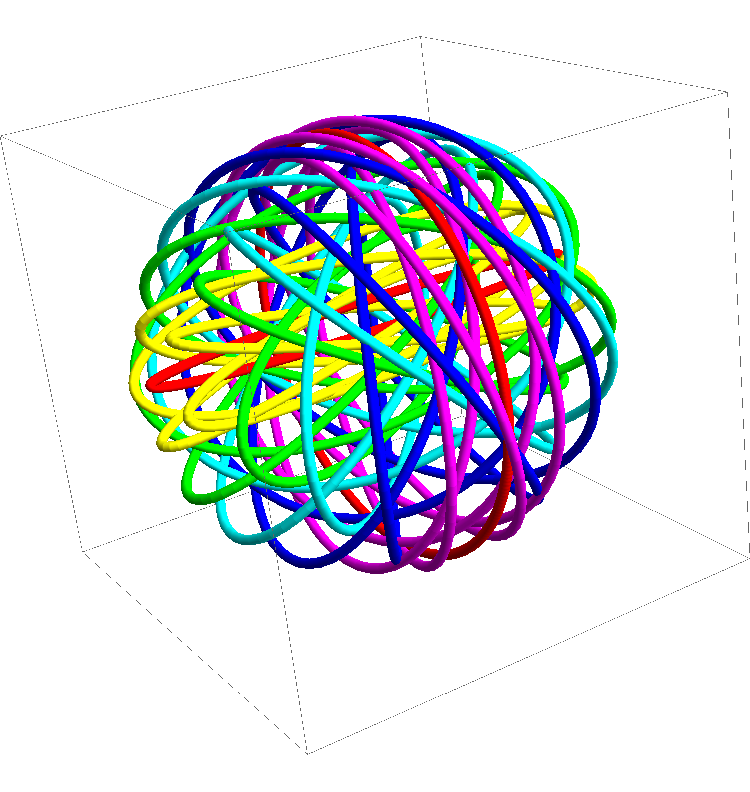
\includegraphics[width=0.48\columnwidth]{hopfFibers}
\par\end{centering}
}\hfill{}\caption{\label{hopfFibers.fig}(a) The two-sphere~$\Sphere{2}$ represented
by \Eq{A7.eq}, which is the irreducible space of one-qubit states,
along with a representative set of points on the sphere. Each single
point on the sphere in (a) corresponding to a circle in (b), and a
whole family of circles (the paths of $\rme^{\rmi\theta}$) on the
three-sphere~$\Sphere{3}$ represents the Hopf fibration, Eq.~(\ref{eq:HopfFibration}).
Although $\Sphere{3}$ cannot be directly embedded in $\R^{3}$, three-sphere~$\Sphere{3}$
can be regarded as attaching two three-dimensional balls on two sides
of two-sphere~$\Sphere{2}$. In this way, each circle in $\Sphere{3}$
can be represented as a circle in the three-dimensional ball as shown
in (b). Moreover, points in (a) are color-coded corresponding to circles
in (b), e.g., one pole contains the red elliptical circle that would
become an infinite-radius circle by a slightly different way to represent
$\Sphere{3}$ in $\R^{3}$, and the opposite pole corresponds to the
large perfectly round red circle at the equator.}
\end{figure}
We can reduce 3 degrees of freedom in Eq.~(\ref{A5.eq}) to 2 degrees
of freedom by effectively removing $\rme^{\rmi\theta}$ (``fibering
out by the circle $\Sphere{1}$''). The standard form of these maps
(``the Hopf fibration'') is 
\begin{eqnarray}
 &  & X=2\,\mathrm{Re}\ \alpha_{0}\alpha_{1}^{*}=2x_{0}x_{1}+2y_{0}y_{1}\,,\nonumber \\
 &  & Y=2\,\mathrm{Im}\ \alpha_{0}\alpha_{1}^{*}=2x_{1}y_{0}-2x_{0}y_{1}\,,\label{eq:HopfFibration}\\
 &  & Z=\left|\alpha_{0}\right|^{2}-\left|\alpha_{1}\right|^{2}={x_{0}}^{2}+{y_{0}}^{2}-{x_{1}}^{2}-{y_{1}}^{2}\,.\nonumber 
\end{eqnarray}
By denoting the three-dimensional vector~$\left(X,Y,Z\right)$ as
$\Hat{a}$, Eq.~(\ref{A5.eq}) implies these transformed coordinates
obeying 
\begin{equation}
\left\Vert \Hat{a}\right\Vert ^{2}=X^{2}+Y^{2}+Z^{2}=\left(\left|\alpha_{0}\right|^{2}+\left|\alpha_{1}\right|^{2}\right)^{2}=1\label{A7.eq}
\end{equation}
and therefore have only two remaining degrees of freedom describing
all possible distinct one-qubit quantum states. In Fig.~\ref{hopfFibers.fig},
we illustrate schematically the family of circles \textit{each one
of which is collapsed to a point}~$\left(\phi,\psi\right)$ on the
surface $X^{2}+Y^{2}+Z^{2}=1$ by the Hopf map.

\begin{figure}[!b]
\begin{centering}
\hfill{}\subfloat[]{\centering{}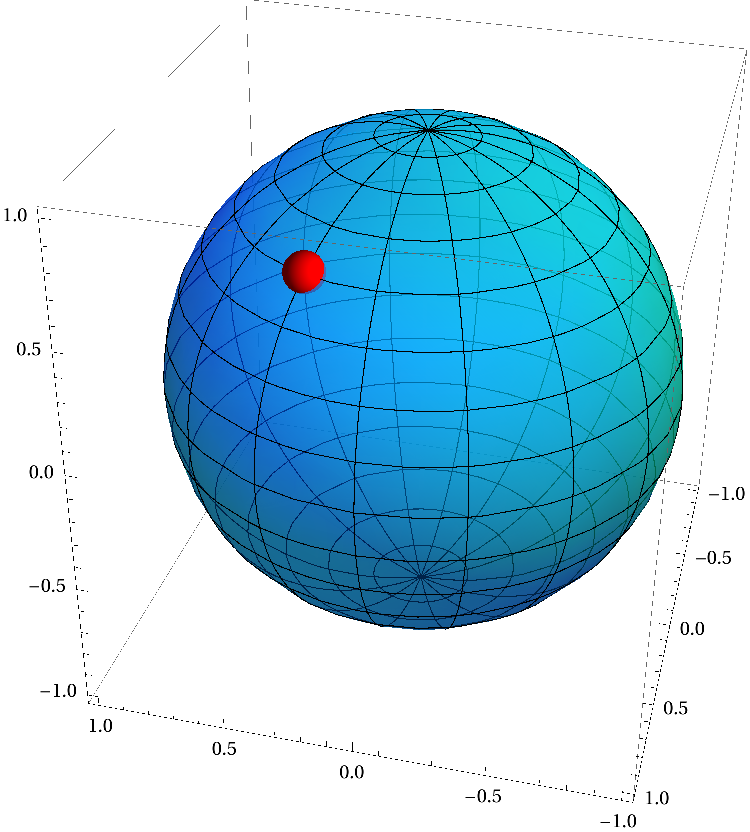
\includegraphics[width=0.47\columnwidth]{blochSphere}}\hfill{}\subfloat[]{\begin{centering}
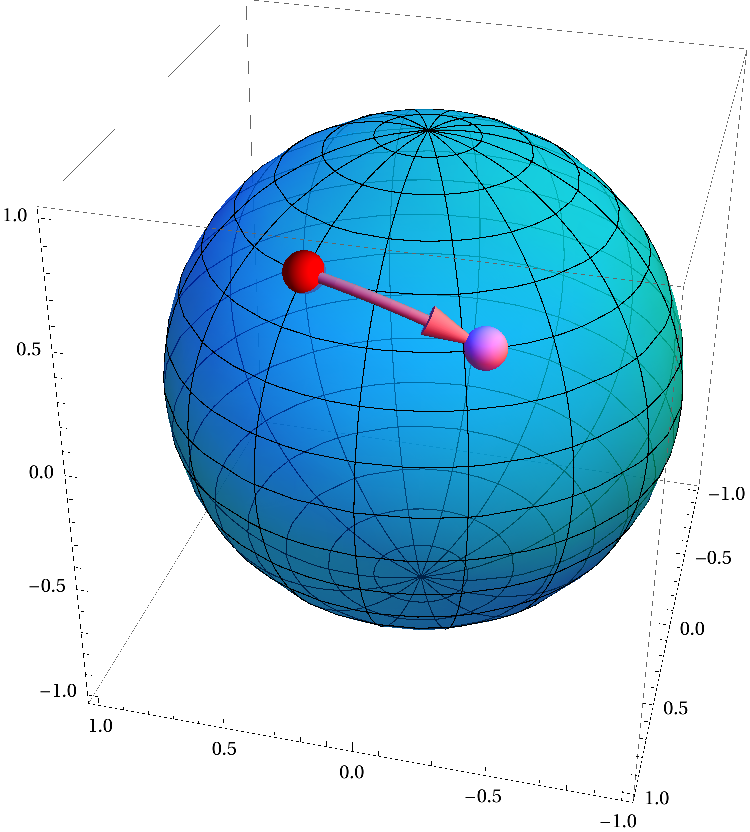
\includegraphics[width=0.47\columnwidth]{blochSphereArc}
\par\end{centering}
}\hfill{}
\par\end{centering}
\caption{\label{blochSphere.fig}(a) The conventional Bloch sphere with a unique
state represented by the point at the red sphere. (b) The geodesic
shortest-distance arc connecting two one-qubit quantum states.}
\end{figure}
The resulting manifold is the two-sphere $\Sphere{2}$ (a 2-manifold)
embedded in $\R^{3}$. If we choose one of many possible coordinate
systems describing $\Sphere{3}$ via Eq.~(\ref{A5.eq}) such as 
\begin{equation}
\left(x_{0},y_{0},x_{1},y_{1}\right)=\left(\cos\left(\theta+\phi\right)\cos\psi,\,\sin\left(\theta+\phi\right)\cos\psi,\,\cos\left(\theta-\phi\right)\sin\psi,\,\sin\left(\theta-\phi\right)\sin\psi\right)\,,\label{A8a.eq}
\end{equation}
where %% $0\leq \theta \leq 2 \pi$,  $-\pi \leq \phi \leq  \pi$, 
$0\leq\psi\leq\frac{\pi}{2}$, with $0\leq\theta+\phi<2\pi$ and $0\leq\theta-\phi<2\pi$,
we see that 
\begin{equation}
\left(X,Y,Z\right)=\left(\cos\left(2\phi\right)\sin\left(2\psi\right),\,\sin\left(2\phi\right)\sin\left(2\psi\right),\,\cos\left(2\psi\right)\right)\,.\label{A8b.eq}
\end{equation}
Thus, the one-qubit state is independent of $\theta$, and we can
choose $\theta=\phi$ without loss of generality, reducing the formula
of the unique one-qubit states to $\ket{\psi_{1}}=\rme^{2\rmi\phi}\cos\psi\ket{0}+\sin\psi\ket{1}$,
and an irreducible state can be represented as a point on a sphere
called the Bloch sphere, as shown in Fig.~\ref{blochSphere.fig}~(a).

Thus, the geometry of a single qubit reduces to transformations among
points on $\Sphere{2}$, which can be parametrized in an infinite
one-parameter family of transformations, one of which is the geodesic
or minimal-length transformation. Explicitly, given two one-qubit
states denoted by points $\Hat{a}$ and $\Hat{b}$ on $\Sphere{2}$,
the shortest rotation carrying $\Hat{a}$ to $\Hat{b}$ is the SLERP
(spherical linear interpolation) \cite{Shoemake:1985:ARQ:325334.325242,wiki:Slerp}
\begin{equation}
S\left(\Hat{a},\Hat{b},t\right)=\Hat{a}\,\frac{\sin((1-t)\omega)}{\sin\omega}\,+\,\Hat{b}\,\frac{\sin(t\omega)}{\sin\omega}\,,\label{slerp.eq}
\end{equation}
where $\Hat{a}\cdot\Hat{b}=\cos\omega$. Figure~\ref{blochSphere.fig}~(b)
illustrates the path traced by a SLERP between two irreducible one-qubit
states on the Bloch sphere. Because states in CQC are defined by infinite
precision real numbers, it is not possible, even in principle, to
make an exact state transition as implied by Fig.~\ref{blochSphere.fig}~(b).
In practice, one must be content with approximate, typically exponentially
expensive, transitions from state to state.

\subsection{$D$-dimensional Hilbert Space}

The irreducible states in a $D$-dimensional Hilbert space are encoded
in a similar family of geometric structures known technically as the
complex projective space $\CP{D-1}$. We obtain these structures starting
with the $D$ initially unnormalized complex coefficients of the $D$-dimensional
basis $\ket{\Psi}=\sum_{i=0}^{D-1}\alpha_{i}\ket{i}$. We then follow
the analog of the two-dimensional procedure: conservation of probability
requires that the norm of the vector $\VVec{\alpha}$ be normalized
to unity: 
\begin{equation}
\braket{\Psi}{\Psi}=\left\Vert \VVec{\alpha}\right\Vert ^{2}=\sum_{i=0}^{D-1}|\alpha_{i}|^{2}=1\,.\label{probEq1.eq}
\end{equation}
Thus, the initial equation for the geometry of a quantum state describes
a \textit{topological sphere~}$\Sphere{2D-1}$ embedded in $\mathReal^{2D}$.
To see this, remember that we can write the real and imaginary parts
of $\alpha_{i}$ as $\alpha_{i}=x_{i}+\rmi y_{i}$, so 
\begin{equation}
\sum_{i=0}^{D-1}|\alpha_{i}|^{2}=\sum_{i=0}^{D-1}{x_{i}}^{2}+{y_{i}}^{2}=1
\end{equation}
describes the locus of a $2D$-dimensional real unit vector in $\mathReal^{2D}$,
which is by definition $\Sphere{2D-1}$, the $(2D-1)$-sphere.

This $\Sphere{2D-1}$ is ambiguous up to the usual overall phase,
inducing an $\Sphere{1}$ symmetry action, and identifying $\Sphere{2D-1}$
as an $\Sphere{1}$ bundle, whose base space is the $(D-1)$-complex-dimensional
projective space $\CP{D-1}$. There are thus $2D-2$ irreducible real
degrees of freedom ($D-1$ complex degrees of freedom) for a quantum
state with a $D$-dimensional basis, $\set{\ket{i}}{i=0,\ldots,D-1}$.

In summary, the full space of a $D$-dimensional quantum state, including
its overall phase defining its relationship to other quantum states,
is the topological space $\Sphere{2D-1}$. For an isolated system,
the overall phase is not measurable, and eliminating the phase dependence
corresponds to identifying $\Sphere{2D-1}$ as a circle bundle over
the base space $\CP{D-1}$, and therefore $\CP{D-1}$ defines the
$2D-2$ intrinsic, irreducible, degrees of freedom of the isolated
$D$-dimensional state's dynamics. In mathematical notation, this
would be written $\Sphere{1}\hookrightarrow\Sphere{2D-1}\rightarrow\CP{D-1}$.
\begin{comment}
\todo{Citation? }
\end{comment}
For $D=2$, the single qubit, we have $2-1=1$, and the base space
of the circle bundle is $\CP{1}=\Sphere{2}$, the usual Bloch sphere.
Note that only for $D=2$ is this actually a sphere-like geometry
due to an accident of low-dimensional topology.

\subsection{Explicit generalization of the Hopf fibration construction\label{subsec:Explicit-generalization-of}}

For a two-dimensional system, we could easily solve the problem of
reducing the full unit-norm space to its irreducible components $\Hat{a}=\left(X,Y,Z\right)$
characterizing the Bloch sphere. We have just argued that essentially
the same process is possible for $D$-dimensional system: in the abstract
argument, we simply identify the family of coefficients $\left\{ \alpha_{i}\right\} $
as being the same if they differ only by an overall phase $\rme^{\rmi\theta}$.
However in practice, this is not a construction that is easy to realize
in a practical computation. We now outline an explicit algorithm for
accomplishing the reduction to the irreducible $D$-dimensional state
space $\CP{D-1}$; this construction will turn out to be useful for
the validation of our discrete results to follow below.

Given a normalized pure state $\ket{\Psi}=\sum_{i=0}^{D-1}\alpha_{i}\ket{i}$,
a natural quantity characterizing a $D$-dimensional system is its
\textit{density matrix}, $\rho=\op{\Psi}{\Psi}$, or 
\begin{equation}
\rho=\begin{pmatrix}|\alpha_{0}|^{2} & \alpha_{0}\alpha_{1}^{*} & \cdots & \alpha_{0}\alpha_{D-1}^{*}\\
\alpha_{1}\alpha_{0}^{*} & |\alpha_{1}|^{2} & \cdots & \alpha_{1}\alpha_{D-1}^{*}\\
\vdots & \vdots & \ddots & \vdots\\
\alpha_{D-1}\alpha_{0}^{*} & \cdots & \alpha_{D-1}\alpha_{D-2}^{*} & |\alpha_{D-1}|^{2}
\end{pmatrix}\,.\label{nqDensity.eq}
\end{equation}
We can now use the complex generalization of the classical Veronese
coordinate system for projective geometry to remove the overall phase
ambiguity $\rme^{\rmi\theta}$ from the $D$-dimensional states. If
we take a particular weighting of the elements of the density matrix~$\rho$,
we can construct a \textit{unit vector} of real dimension $D^{2}$
with the form: 
\begin{equation}
\Hat{a}=\left(|\alpha_{i}|^{2},\ldots,\sqrt{2}\,\mathrm{Re}\ \alpha_{i}\alpha_{j}^{*},\ldots,\sqrt{2}\,\mathrm{Im}\ \alpha_{i}\alpha_{j}^{*},\ldots\right)\,,\label{nqCoords.eq}
\end{equation}
where 
\[
\Hat{a}\cdot\Hat{a}=\sum_{i=0}^{D-1}\left(\left|\alpha_{i}\right|^{2}\right)^{2}+\sum_{i=0}^{D-1}\sum_{\substack{j=0\\
j\ne i
}
}^{D-1}\left(\mathrm{Re}\ \alpha_{i}\alpha_{j}^{*}\right)^{2}+\left(\mathrm{Im}\ \alpha_{i}\alpha_{j}^{*}\right)^{2}=\left(\sum_{i=0}^{D-1}\left|\alpha_{i}\right|^{2}\right)\left(\sum_{j=0}^{D-1}\left|\alpha_{j}\right|^{2}\right)=1\,.
\]
This construction gives an explicit embedding of the $\left(D-1\right)$-dimensional
complex, or $\left(2D-2\right)$-dimensional real, object in a real
space of dimension $D^{2}$. However, this is somewhat subtle because
the vector is of unit length, so technically the embedding space is
a sphere of dimension $D^{2}-1$ embedded in $\R^{D^{2}}$. For example,
the two-dimensional irreducible states could be represented in a four-dimensional
embedding, but the magnitude of every coordinate would be one. Furthermore,
the object embedded in the resulting $\Sphere{3}$ is indeed $\Sphere{2}$
because we can fix one complex coordinate to be unity, and let one
vary, giving a total of two irreducible dimensions. In fact, one must
choose \textit{two} coordinate patches, one covering one pole of $\Sphere{2}$
with coordinates $\alpha_{0}=1+\rmi0$ and $\alpha_{1}=x_{1}+\rmi y_{1}$,
and the other patch covering the other pole of $\Sphere{2}$ with
coordinates $\alpha_{0}=x_{0}+\rmi y_{0}$ and $\alpha_{1}=1+\rmi0$.
\begin{comment}
\todo{Explain the last part clearer or add a picture.}
\end{comment}

We finally see that the irreducible $D$-dimensional state space $\CP{D-1}$
is described by $D$ projectively equivalent coordinates, one of which
can always be scaled out to leave $(D-1)$ actual (complex) degrees
of freedom. We must choose, in turn, $D$ different local sets of
complex variables defined by taking the value $\alpha_{k}=1$, with
$k=0,\ldots,D-1$, and allowing the remaining $D-1$ complex (or $2D-2$
real) variables to run free. No single set of coordinates will work,
since the submanifold including $\alpha_{k}=0$ is undefined and another
coordinate system must be chosen to cover that coordinate patch. This
is a standard feature of the topology of non-trivial manifolds such
as $\CP{D-1}$ (see any textbook on geometry~\cite{Berger_1988}).

\section{Quantum Probability\label{sec:fuzzy}}

A \emph{probability space} is a mathematical abstraction specifying
the necessary conditions for reasoning coherently about collections
of uncertain events \cite{Kolmogorov1950,544199,Griffiths2003,Grabisch2016}.
Although they can be used to describe an individual quantum experiment,
to describe a family of quantum experiments, we would like to glue
their probability spaces together to define a quantum probability
space. The glued quantum probability space is well-behaved since not
only we can define the expectation values, but the quantum probability
measure defined on the whole space can be simply induced by the Born
rule according to Gleason's theorem \cite{gleason1957,Redhead1987-REDINA,peres1995quantum,RichmanBridges1999,Hamhalter2013}.

\subsection{Classical and Quantum Probability Spaces\label{subsec:Classical-and-Quantum}}

Given a finite sample space~$\Omega$ representing all possible outcomes
of a process, and its power set $2^{\Omega}$ as the classical event
space, a classical probability measure~$\mu$ maps every event $E\subseteq\Omega$
to a number $\mu\left(E\right)\in\left[0,1\right]$ specifying how
likely one of the outcomes in $E$ will happen. To maintain the coherence,
$\mu$ is subject to the following constraints: $\mu\left(\emptyset\right)=0$,
$\mu\left(\Omega\right)=1$, and $\mu\left(\overline{E}\right)=1-\mu\left(E\right)$,
where $\overline{E}$ is the complement of $E$.  Moreover, we require
$\mu\left(E_{0}\cup E_{1}\right)=\mu\left(E_{0}\right)+\mu\left(E_{1}\right)$
for each pair of disjoint events $E_{0}\subseteq\Omega$ and $E_{1}\subseteq\Omega$.

Since the previous abstraction doesn't specify the process to generate
the outcomes, this process could well be a quantum experiment. Let
us prepare a beam of one kind of spin~$1$ particles whose state
can be characterized by a vector in three-dimensional Hilbert space
with basis vectors $\ket{0}$, $\ket{1}$, and $\ket{2}$. In principle,
this beam can be split by a Stern-Gerlach type experiment according
to the eigenvalues of the observable $\mathbf{O}_{0}$ with spectral
decomposition 
\begin{equation}
\mathbf{O}_{0}=0\,\proj{0}+1\,\proj{1}+2\,\proj{2}\,,\label{eq:observable}
\end{equation}
and the states corresponding to the split beams are $\ket{0}$, $\ket{1}$,
and $\ket{2}$ \cite{:/content/aip/journal/jmp/21/1/10.1063/1.524312,peres1995quantum}.
Instead of sending a beam of particles, if only one particle is sent
to the beam splitter, the state of the particle after the experiment
is one of $\ket{0}$, $\ket{1}$, and $\ket{2}$, and there is a probability
to get each post-experimental state. In the language of our abstraction,
the set of outcomes is $\Omega_{0}=\left\{ \ket{0},\ket{1},\ket{2}\right\} $.
All possible events are $\emptyset$, $\left\{ \ket{0}\right\} $,
$\left\{ \ket{1}\right\} $, $\left\{ \ket{2}\right\} $, $\left\{ \ket{0},\ket{1}\right\} $,
$\left\{ \ket{0},\ket{2}\right\} $, $\left\{ \ket{1},\ket{2}\right\} $,
and $\Omega_{0}$. And this experiment defines a classical probability
measure $\mu_{0}\colon2^{\Omega_{0}}\rightarrow\left[0,1\right]$.

One special feature of quantum experiments is that the probabilities
in different experiments are correlated. Consider another experiment
sending exactly the same particle as the previous one but using a
different beam splitter corresponding to the observable $\mathbf{O}_{1}$
with spectral decomposition $\mathbf{O}_{1}=0\,\proj{\ps}+1\,\proj{\ms}+2\,\proj{2}$,
where $\ket{\ps}=\frac{\ket{0}+\ket{1}}{\sqrt{2}}$ and $\ket{\ms}=\frac{\ket{0}-\ket{1}}{\sqrt{2}}$.
Although the sample space $\Omega_{1}=\left\{ \ket{\ps},\ket{\ms},\ket{2}\right\} $
and the probability measure $\mu_{1}\colon2^{\Omega_{1}}\rightarrow\left[0,1\right]$
defined by this experiment is different from the previous one, these
two experiments may produce the same post-experimental state~$\ket{2}$,
and the probability of the common event $\left\{ \ket{2}\right\} $
is believed to be the same, i.e., 
\begin{equation}
\mu_{0}\left(\left\{ \ket{2}\right\} \right)=\mu_{1}\left(\left\{ \ket{2}\right\} \right)\,.\label{eq:mu0-equal-mu1}
\end{equation}
In general, as long as sending the same particle, the probability
of the same event in different experiments should always be the same.
This fact is equivalent to the fact that commuting observables could
be measured simultaneously which is essential to define contextuality
and will be explained in Sec.~\ref{sec:Kochen-Specker}.

Since the probability induced by the different beam splitters are
correlated, it is more natural to define one quantum event space~$\events$
containing all possible classical event spaces using different beam
splitters. However, simply taking the union of all event spaces is
a bad idea because two events might appear different but represent
the same situation. For example, if we take the complement on both
sides of Eq.~(\ref{eq:mu0-equal-mu1}), we will have
\begin{equation}
\mu_{0}\left(\left\{ \ket{0},\ket{1}\right\} \right)=1-\mu_{0}\left(\left\{ \ket{2}\right\} \right)=1-\mu_{1}\left(\left\{ \ket{2}\right\} \right)=\mu_{1}\left(\left\{ \ket{\ps},\ket{\ms}\right\} \right)\,,
\end{equation}
that is, the probabilities of events $\left\{ \ket{0},\ket{1}\right\} $
and $\left\{ \ket{\ps},\ket{\ms}\right\} $ are always the same, and
these events should be identified as the same quantum event to simplify
our discussion. This identification can be achieved by mapping a classical
event~$E$ to the projector generated by $E$,
\begin{equation}
\varphi\left(E\right)=\sum_{\ket{j}\in E}\proj{j}\label{eq:pullback-function}
\end{equation}
with the convention $\varphi\left(\emptyset\right)=\mathbb{0}$, because
$\varphi\left(\left\{ \ket{0},\ket{1}\right\} \right)$ is equal to
$\varphi\left(\left\{ \ket{\ps},\ket{\ms}\right\} \right)$ as operators,
\begin{equation}
\varphi\left(\left\{ \ket{0},\ket{1}\right\} \right)=\proj{0}+\proj{1}=\proj{\ps}+\proj{\ms}=\varphi\left(\left\{ \ket{\ps},\ket{\ms}\right\} \right)\,.
\end{equation}
In general, if two classical events~$E$ and $E'$ are mapped to
the same projector, i.e., $\varphi\left(E\right)=\varphi\left(E'\right)$,
then the probability of $E$ is the same as the probability of $E'$.
Therefore, for any classical event~$E$, its corresponding quantum
event is defined to be the projector $\varphi\left(E\right)$, and
the set of all projectors on a given Hilbert space is called a quantum
event space~$\events$. %
\begin{comment}
\todo{Check the citation of this part. Did von Neumann really think
about this when he uses projectors to formulate the quantum theory?}
\end{comment}

This function $\varphi$ not only respects the probability of events
but also naturally sends the set structure to the corresponding projector
structure:
\begin{align}
\varphi\left(\Omega\right) & =\mathbb{1}\,, & \varphi\left(\overline{E}\right) & =\mathbb{1}-\varphi\left(E\right)\,.\label{eq:pullback-properties-basic}
\end{align}
Given two \emph{commuting} projectors $P_{0}$ and~$P_{1}$, there
exists a pair of events $E_{0}$ and $E_{1}$ in the same sample space~$\Omega$
such that $P_{0}=\varphi\left(E_{0}\right)$ and $P_{1}=\varphi\left(E_{1}\right)$.
Conversely, given a pair of events $E_{0}$ and $E_{1}$ in the same
sample space~$\Omega$, their corresponding quantum events $\varphi\left(E_{0}\right)$
and $\varphi\left(E_{1}\right)$ are commuting and satisfying the
following properties: 
\begin{align}
\varphi\left(E_{0}\cap E_{1}\right) & =\varphi\left(E_{0}\right)\varphi\left(E_{1}\right)\,, & \varphi\left(E_{0}\cup E_{1}\right) & =\varphi\left(E_{0}\right)+\varphi\left(E_{1}\right)-\varphi\left(E_{0}\right)\varphi\left(E_{1}\right)\,.\label{eq:pullback-properties}
\end{align}
Moreover, $E_{0}$ and $E_{1}$ are disjoint if and only if $\varphi\left(E_{0}\right)$
and $\varphi\left(E_{1}\right)$ are orthogonal, where two projectors
$P_{0}$ and $P_{1}$ are called \emph{orthogonal} if $P_{0}P_{1}=\mathbb{0}$.

Then, a quantum probability space can be defined as a quantum event
space~$\events$ together with a quantum probability measure $\mu\colon\events\rightarrow\left[0,1\right]$
subject to the corresponding constraints \cite{10.2307/2308516,gleason1957,Redhead1987-REDINA,Maassen2010,Abramsky2012}:
\begin{align}
\mu\left(\mathbb{0}\right) & =0\,, & \mu\left(\mathbb{1}\right) & =1\,, & \mu\left(\mathbb{1}-P\right) & =1-\mu\left(P\right)\,,\label{eq:QuantumProbability}
\end{align}
and for each pair of orthogonal projectors $P_{0}$ and $P_{1}$:
\begin{equation}
\mu\left(P_{0}+P_{1}\right)=\mu\left(P_{0}\right)+\mu\left(P_{1}\right)\,.\label{eq:QuantumProbability-Addition}
\end{equation}
Because $\varphi$ respects the probability of events, if we restrict
the domain of $\varphi$ on a classical event space $2^{\Omega}$,
the function $\varphi^{*}\mu\colon2^{\Omega}\rightarrow\left[0,1\right]$
defined by precomposition 
\begin{equation}
\left(\varphi^{*}\mu\right)\left(E\right)=\mu\left(\varphi\left(E\right)\right)\label{eq:classical-pullback}
\end{equation}
is a classical probability measure and called the pullback of $\mu$
by $\varphi\colon2^{\Omega}\rightarrow\events$.

Given a Hilbert space $\mathcal{H}$ of dimension $D$ and a probability
assignment for every projector $P$, we can define the expectation
value of an observable~$\mathbf{O}$ having spectral decomposition
$\mathbf{O}=\sum_{i=0}^{D-1}\lambda_{i}P_{i}$, with eigenvalues $\lambda_{i}\in\mathbb{R}$,
as \cite{544199,Jaeger2007}: 
\begin{equation}
\expval{\mathbf{O}}_{\mu}=\sum_{i=0}^{D-1}\lambda_{i}\mu\left(P_{i}\right)\,,\label{eq:quantum-expectation}
\end{equation}
where the subscript $\mu$ might be omitted if it is clear according
to the context. This definition is also consistent with the classical
expectation values because we can pullback an observable to a classical
random variable, and the expectation values are invariant.%
\begin{comment}
\todo{ Add interpretation!}
\end{comment}

\begin{definition}[Pullback of Observables]\label{def:observable2random-variable}Consider
an observable~$\mathbf{O}$ diagonalizable by an orthonormal basis
$\Omega=\{\ket{0},\ket{1},\ldots,\ket{D-1}\}$ so that $\mathbf{O}$
has spectral decomposition $\mathbf{O}=\sum_{i=0}^{D-1}\lambda_{i}\proj{i}$.
If we restrict $\varphi$ on the classical event space~$2^{\Omega}$
and consider $\varphi\colon2^{\Omega}\rightarrow\events$, then the
pullback of $\mathbf{O}$ by $\varphi$ is a random variable $\varphi^{*}\mathbf{O}\colon\Omega\rightarrow\mathbb{R}$
defined by $\varphi^{*}\mathbf{O}=\sum_{i=0}^{D-1}\lambda_{i}\mathbf{1}_{\left\{ \ket{i}\right\} }$,
where $\mathbf{1}_{E}$ is the indicator function defined by
\begin{equation}
\mathbf{1}_{E}\left(\omega\right)=\begin{cases}
1 & \textrm{if }\omega\in E\,;\\
0 & \textrm{if }\omega\notin E\,.
\end{cases}
\end{equation}
\begin{comment}
\todo{Put the definition of indicator function!}
\end{comment}
\end{definition}

\begin{lemma}\label{lemma:real-expectation-value-between-classical-quantum}Consider
an observable~$\mathbf{O}$ diagonalizable by an orthonormal basis
$\Omega=\{\ket{0},\ket{1},\ldots,\ket{D-1}\}$ with $\varphi\colon2^{\Omega}\rightarrow\events$
defined by Eq.~(\ref{eq:pullback-function}). Given a quantum probability
measure $\mu\colon\events\rightarrow\left[0,1\right]$, the expectation
value of $\mathbf{O}$ relative to $\mu$ is exactly the expectation
value of the pullback of $\mathbf{O}$ relative to the pullback of
$\mu$, i.e., 
\begin{equation}
\expval{\mathbf{O}}_{\mu}=\int\left(\varphi^{*}\mathbf{O}\right)\rmd\left(\varphi^{*}\mu\right)\,.\label{eq:real-expectation-value-between-classical-quantum}
\end{equation}
\end{lemma}

\begin{proof}By Eqs.~(\ref{eq:quantum-expectation}), (\ref{eq:pullback-function}),
and (\ref{eq:classical-pullback}), we have
\[
\expval{\mathbf{O}}_{\mu}=\sum_{i=0}^{D-1}\lambda_{i}\mu\left(\proj{i}\right)=\sum_{i=0}^{D-1}\lambda_{i}\mu\left(\varphi\left(\left\{ \ket{i}\right\} \right)\right)=\sum_{i=0}^{D-1}\lambda_{i}\left(\varphi^{*}\mu\right)\left(\left\{ \ket{i}\right\} \right)=\int\left(\varphi^{*}\mathbf{O}\right)\rmd\left(\varphi^{*}\mu\right)\,.
\]
\end{proof}

\subsection{Gleason's Theorem and the Born Rule\label{subsec:Gleason's-Theorem-and}}

After introducing quantum probability measures, we might follow the
convention to introduce the Born rule which is the only way to relate
a state to a quantum probability measure in CQT\@. However, since
the variants of quantum probability measures in Sec.~\ref{sec:Toward-IVPM}
and Chapter~\ref{chap:QIVPM} could not be constructed by a ``Born
rule'' easily, searching for a Born rule step-by-step here might
provide a better idea of what we should do in Sec.~\ref{sec:Toward-IVPM}
and Chapter~\ref{chap:QIVPM}. While the situations will become more
delicate in the later sections, we will fortunately find the unique
Born rule for CQT here.

Although the quantum probability measure constructed by gluing together
classical ones looks complex, it could be induced by an operator according
to Gleason's theorem \cite{gleason1957,Redhead1987-REDINA,peres1995quantum,RichmanBridges1999,Hamhalter2013}.

\begin{thm}[Gleason's theorem]\label{cor:Gleason's}In a Hilbert
space $\Hilb$ of dimension $D\geq3$, given a quantum probability
measure $\mu\colon\events\rightarrow\left[0,1\right]$, there exists
a unique mixed state $\rho=\sum_{j=1}^{N}q_{j}\proj{\Phi_{j}}$ such
that $\mu\left(P\right)=\Tr\left(\rho P\right)$ for any $D$-dimensional
projector~$P$, where $\ket{\Phi_{j}}\in\mathcal{H}$ are normalized,
$q_{j}>0$, and $\sum_{j=1}^{N}q_{j}=1$.\end{thm}

If we follow the discussion of Stern-Gerlach type experiments in the
previous section to interpret Gleason's theorem, we can find Gleason's
theorem doesn't specify whether its unique mixed state~$\rho$ characterizes
the state of particle sending to the quantum experiment or not. Consider
an extreme example: a quantum theory could ignore the input state
and predict the experimental outcomes are always equally probable.
Even if these predictions form a quantum probability measure, this
kind of prediction is so different from the prediction of CQT that
they can be easily distinguished experimentally.

Let a pure unnormalized state $\ket{\Phi}\in\mathcal{H}$ characterize
the particle sending to a Stern-Gerlach type experiment, and $\muB_{\Phi}$
be the quantum probability measure of the resulting events sensibly
corresponding to $\ket{\Phi}$. For a correspondence $\ket{\Phi}\mapsto\muB_{\Phi}$
to be sensible, we hope that if the state~$\ket{\Phi}$ is one of
the outcomes of a quantum event~$P$, $P\ket{\Phi}=\ket{\Phi}$,
then the event~$P$ always happens, 
\begin{equation}
\muB_{\Phi}\left(P\right)=1\,,\label{eq:Born-probability-one}
\end{equation}
and vice versa. Moreover, since the physical phenomena exist and should
be the same no matter how we describe them, the probability of an
event should be invariant despite how we choose the basis. Because
changing to another basis is the same as applying a unitary map~$U$,
we should have 
\begin{equation}
\muB_{U\ket{\Phi}}\left(UPU^{\dagger}\right)=\muB_{\Phi}\left(P\right)\,.\label{eq:Born-unitary-invariant}
\end{equation}
It is easy to check that the correspondence satisfying these conditions
is unique, 
\begin{equation}
\muB_{\Phi}(P)=\frac{\melem{\Phi}{P}{\Phi}}{\ip{\Phi}{\Phi}}\label{eq:Born}
\end{equation}
and called the Born rule \cite{Born1983,Mermin2007,Jaeger2007}. If
$\ket{\Phi}$ is normalized, Eq.~(\ref{eq:Born}) could be simplified
as $\muB_{\Phi}(P)=\melem{\Phi}{P}{\Phi}$. Since a mixed state $\rho=\sum_{j=1}^{N}q_{j}\proj{\Phi_{j}}$
is a weighted average of projectors $\proj{\Phi_{j}}$ with weights
$q_{j}>0$ and $\sum_{j=1}^{N}q_{j}=1$, the generalized Born rule
of $\rho$, $\muB_{\rho}\left(P\right)$, is also a weighted average
of $\muB_{\Phi_{j}}\left(P\right)$, 
\begin{equation}
\muB_{\rho}\left(P\right)=\sum_{j=1}^{N}q_{j}\muB_{\Phi_{j}}\left(P\right)=\Tr\left(\rho P\right)\,,\label{eq:mixed-Born}
\end{equation}
which is also a quantum probability measure and consistent with Gleason's
theorem.

As an example, consider a three-dimensional Hilbert space with orthonormal
basis $\left\{ \ket{0},\ket{1},\ket{2}\right\} $ and the observable
$\mathbf{O}_{0}$ defined in Eq.~(\ref{eq:observable}). Two fragments
of valid probability measures~$\mu_{1}$ and $\mu_{2}$ that can
be associated with this space are defined in Table~\ref{tab:quantum-probability-measure}.
By the Born rule, the first probability measure corresponds to the
quantum system being in the pure state $\ket{\ps}=\frac{\ket{0}+\ket{1}}{\sqrt{2}}$
and the second corresponds to the quantum system being in the state
$\frac{\proj{0}+\proj{2}}{2}$. The expectation values of the observable
$\mathbf{O}$, $\expval{\mathbf{O}}_{\mu_{1,2}}$, are $1.5$ in the
first case and $2$ in the second. The quantum expectation value can
also be used to decide whether a state is entangled or not for multipartite
systems as we describe in the following section.
\begin{table}
\begin{doublespace}
\noindent \centering{}\caption{\label{tab:quantum-probability-measure}Two fragments of valid probability
measures~$\mu_{1}$ and $\mu_{2}$.}
\begin{tabular}{ccccccccccc}
\toprule 
$\ket{\Psi}$ & $\ket{0}$ & $\ket{1}$ & $\ket{2}$ & $\frac{\ket{0}+\ket{1}}{\sqrt{2}}$ & $\frac{\ket{0}+\rmi\ket{1}}{\sqrt{2}}$ & $\frac{\ket{0}+\ket{2}}{\sqrt{2}}$ & $\frac{\ket{0}+\rmi\ket{2}}{\sqrt{2}}$ & $\frac{\ket{1}+\ket{2}}{\sqrt{2}}$ & $\frac{\ket{1}+\rmi\ket{2}}{\sqrt{2}}$ & $\cdots$\tabularnewline
\midrule
$\mu_{1}\left(\proj{\Psi}\right)$ & $\frac{1}{2}$ & $\frac{1}{2}$ & $0$ & $1$  & $\frac{1}{2}$ & $\frac{1}{4}$ & $\frac{1}{4}$ & $\frac{1}{4}$ & $\frac{1}{4}$ & $\cdots$\tabularnewline
$\mu_{2}\left(\proj{\Psi}\right)$ & $\frac{1}{2}$ & $0$ & $\frac{1}{2}$ & $\frac{1}{4}$ & $\frac{1}{4}$ & $\frac{1}{2}$ & $\frac{1}{2}$ & $\frac{1}{4}$ & $\frac{1}{4}$ & $\cdots$\tabularnewline
\bottomrule
\end{tabular}
\end{doublespace}
\end{table}


\section{The geometry of entanglement\label{sec:The-geometry-of}}

Entanglement may be regarded as one of the main characteristics distinguishing
quantum from classical mechanics. Entanglement involves quantum correlations
such that the measurement outcomes in one subsystem are related to
the measurement outcomes in another one. To discuss entanglement,
we consider a $D$-dimensional quantum system composed of $n$-qubit
subsystems, i.e., $D=2^{n}$. A pure state of the total system $\ket{\Psi}$
is said to be entangled if it cannot be written as a product of states
of each subsystem \cite{peres1995quantum,544199,Jaeger2007}. That
is, a state $\ket{\Psi}$ is entangled if $\ket{\Psi}\ne\ket{\psi_{1}}\otimes\cdots\otimes\ket{\psi_{j}}\otimes\cdots\otimes\ket{\psi_{n}}$,
where $\ket{\psi_{j}}$ refers to an arbitrary state of the $j$-th
qubit, and $\otimes$ represents the tensor product. This is equivalent
to saying that if one calculates the reduced density operator~$\rho_{j}$
of the $j$-th subsystem by tracing out all the other subsystems,
\begin{equation}
\rho_{j}=\Tr_{\left\{ 1,\ldots,j-1,j+1,\ldots,n\right\} }\left(\rho\right)\,,\label{eq:partialTrace}
\end{equation}
with $j=1,\ldots,n$ and $\rho=\op{\Psi}{\Psi}$, the normalized state~$\ket{\Psi}$
is entangled if and only if at least one subsystem state is \textit{mixed},
i.e., $\Tr_{j}\left(\rho_{j}^{2}\right)<1$ \cite{544199,Jaeger2007}.

The reduced density operator could be expressed explicitly by the
expectation value of the Pauli operators. Therefore, we can decide
whether a system is entangled or not by examining these expectation
values. Let $\jthSubsystem{\sigma}[\eta]{j}$ be the Pauli operators
acting on the $j$-th spin~\cite{544199},
\begin{equation}
\jthSubsystem{\sigma}[\eta]{j}=\overbrace{\sigma_{0}\otimes\cdots\otimes\sigma_{0}\otimes\underbrace{\sigma_{\eta}}_{j^{\textrm{th}}\textrm{ factors}}\otimes\sigma_{0}\otimes\cdots\otimes\sigma_{0}}^{n\textrm{ factors}}\,,\label{pauli3}
\end{equation}
and $\expval{\jthSubsystem{\sigma}[\eta]{j}}$ be the corresponding
expectation value, $\expval{\jthSubsystem{\sigma}[\eta]{j}}=\melem{\Psi}{\jthSubsystem{\sigma}[\eta]{j}}{\Psi}$,
where $\eta=x$, $y$, and $z$, and
\begin{subequations}
\begin{align}
\sigma_{0} & =\op{0}{0}+\op{1}{1}\,, & \sigma_{x} & =\op{1}{0}+\op{0}{1}\,,\\
\sigma_{y} & =\rmi\op{1}{0}-\rmi\op{0}{1}\,, & \sigma_{z} & =\op{0}{0}-\op{1}{1}\,.
\end{align}
\end{subequations}
For example, given a normalized two-qubit system $\ket{\Psi}=\alpha_{00}\ket{00}+\alpha_{01}\ket{01}+\alpha_{10}\ket{10}+\alpha_{11}\ket{11}$,
some of its expectation values are
\begin{equation}
\begin{aligned}\expval{\jthSubsystem{\sigma}[0]{1}} & =\left|\alpha_{00}\right|^{2}+\left|\alpha_{01}\right|^{2}+\left|\alpha_{10}\right|^{2}+\left|\alpha_{11}\right|^{2}=1\,,\\
\expval{\jthSubsystem{\sigma}[x]{1}} & =\alpha_{00}\alpha_{10}^{*}+\alpha_{01}\alpha_{11}^{*}+\alpha_{10}\alpha_{00}^{*}+\alpha_{11}\alpha_{01}^{*}\,,\\
\expval{\jthSubsystem{\sigma}[y]{1}} & =-\alpha_{00}\alpha_{10}^{*}\rmi-\alpha_{01}\alpha_{11}^{*}\rmi+\alpha_{10}\alpha_{00}^{*}\rmi+\alpha_{11}\alpha_{01}^{*}\rmi\,,\\
\expval{\jthSubsystem{\sigma}[z]{1}} & =\left|\alpha_{00}\right|^{2}+\left|\alpha_{01}\right|^{2}-\left|\alpha_{10}\right|^{2}-\left|\alpha_{11}\right|^{2}\,.
\end{aligned}
\end{equation}
Then, the reduced density operator~$\rho_{1}$ can be expressed by
these expectation values as following:
\begin{equation}
\begin{aligned}\rho_{1}= & \Tr_{\left\{ 2\right\} }\left(\op{\Psi}{\Psi}\right)\\
= & \left(\left|\alpha_{00}\right|^{2}+\left|\alpha_{01}\right|^{2}\right)\op{0}{0}+\left(\alpha_{00}\alpha_{10}^{*}+\alpha_{01}\alpha_{11}^{*}\right)\op{0}{1}\\
 & +\left(\alpha_{10}\alpha_{00}^{*}+\alpha_{11}\alpha_{01}^{*}\right)\op{1}{0}+\left(\left|\alpha_{10}\right|^{2}+\left|\alpha_{11}\right|^{2}\right)\op{1}{1}\\
= & \frac{\expval{\jthSubsystem{\sigma}[0]{1}}\sigma_{0}+\expval{\jthSubsystem{\sigma}[x]{1}}\sigma_{x}+\expval{\jthSubsystem{\sigma}[y]{1}}\sigma_{y}+\expval{\jthSubsystem{\sigma}[z]{1}}\sigma_{z}}{2}\,.
\end{aligned}
\end{equation}
In general, %
\begin{comment}
\todo{Ask Gerardo why? }
\end{comment}
the reduced density operator~$\rho_{j}$ of the $j$-th subsystem
can always be expressed as
\begin{equation}
\rho_{j}=\frac{1}{2}\sum\limits _{\eta=0,x,y,z}\expval{\jthSubsystem{\sigma}[\eta]{j}}\sigma_{\eta}\,,\label{eq:reducedDensityOperator}
\end{equation}
and its coefficients can be summarized as the vector
\begin{equation}
{\bf X}_{j}=\left(\expval{\jthSubsystem{\sigma}[x]{j}},\expval{\jthSubsystem{\sigma}[y]{j}},\expval{\jthSubsystem{\sigma}[z]{j}}\right)\in\mathbb{R}^{3}\label{eq:geometricRepresentationState}
\end{equation}
that allows a geometric representation of each reduced state in $\mathbb{R}^{3}$,
satisfying $0\le\left\Vert {\bf X}_{j}\right\Vert \le1$. Since $\Tr_{j}\left(\rho_{j}^{2}\right)=\frac{1}{2}\left(1+\left\Vert {\bf X}_{j}\right\Vert ^{2}\right)$,
the state $\ket{\Psi}$ is entangled if $\left\Vert {\bf X}_{j}\right\Vert <1$
for at least one $j$, represented by a point \emph{inside} the corresponding
local Bloch sphere embedded in $\mathbb{R}^{3}$. Therefore, one may
consider $\ket{\Psi}$ to be maximally entangled if $\left\Vert {\bf X}_{j}\right\Vert =0$
for all $j$. On the other hand, the state $\ket{\Psi}$ is unentangled
(i.e., a product state) if $\left\Vert {\bf X}_{j}\right\Vert =1$
for all $j$, corresponding to points lying on the surface of the
Bloch spheres.

A natural geometric measure of multipartite entanglement is obtained
by defining the \emph{purity of a state relative to a set of observables}
\cite{BKOV2003,BKOSV2004}. If the set is chosen to be the set of
\emph{all local observables}, i.e., corresponding to each of the subsystems
that compose the actual system, one recovers the standard notion of
entanglement for multipartite systems. For example, if the system
consists of $n$ qubits, we obtain a measure of conventional entanglement
by calculating the purity relative to the semi-simple Lie algebra~$\fh$
spanned by $\{\jthSubsystem{\sigma}[x]{1},\jthSubsystem{\sigma}[y]{1},\jthSubsystem{\sigma}[z]{1},\ldots,\jthSubsystem{\sigma}[x]{n},\jthSubsystem{\sigma}[y]{n},\jthSubsystem{\sigma}[z]{n}\}$,
\begin{equation}
P_{\fh}=\frac{1}{n}\sum\limits _{j=1}^{n}\sum\limits _{\eta=x,y,z}\expval{\jthSubsystem{\sigma}[\eta]{j}}^{2}=\frac{1}{n}\sum\limits _{j=1}^{n}\left\Vert {\bf X}_{j}\right\Vert ^{2}\,.\label{purityMeasure.eq}
\end{equation}
Since the norm of the geometric representation state $\left\Vert {\bf X}_{j}\right\Vert $
defined in Eq.~(\ref{eq:geometricRepresentationState}) is between
$0$ and $1$, we have $0\leq P_{\fh}\leq1$, where $\frac{1}{n}$
in Eq.~(\ref{purityMeasure.eq}) is just a normalization factor.
All the product states of the form $\ket{\Psi}=\ket{\psi_{1}}\otimes\cdots\otimes\ket{\psi_{n}}$,
have maximum purity (i.e., $P_{\fh}=1$). Other states such as the
Greenberger-Horne-Zeilinger state $\ket{\Psi}=\ket{\mathsf{GHZ}_{n}}=\frac{1}{\sqrt{2}}\left(\ket{0}\otimes\cdots\otimes\ket{0}+\ket{1}\otimes\cdots\otimes\ket{1}\right)$
are (maximally) entangled relative to the set of local observables
(i.e., $P_{\fh}=0$).

Different entanglement measures are obtained when an algebra~$\fh$
different from the local observables is chosen. An obvious example
is given by the set of all observables. In this case, the purity takes
its maximum value independently of the pure quantum state \cite{BKOV2003,BKOSV2004},
expressing the fact that any state is a generalized coherent state
of the Lie algebra of all observables.

\chapter{Quantum Theories and Computing over Unrestricted Finite Fields\label{chap:Unrestricted-Finite-Fields}}

\section{Fundamentals of Finite Fields\label{sec:background}}

\subsection{Background}

A field~$\mathbb{F}$ is an algebraic structure consisting of a set
of elements equipped with the operations of addition, subtraction,
multiplication, and division \cite{DummitFoote2004,fieldtheory.ref,numtheory.ref}.
Fields may contain an infinite or a finite number of elements. The
rational~$\mathbb{Q}$, real~$\mathbb{R}$, and complex numbers~$\mathbb{C}$
are examples of infinite fields, while the set $\mathbb{F}_{3}=\{0,1,2\}$,
under multiplication and addition modulo $3$, is an example of a
finite field.

There are two distinguished elements in a field, the addition identity
$0$, and the multiplication identity $1$. Given the field~$\mathbb{F}$,
the closed operations of addition~$+$, and multiplication~$\gmult$,
satisfy the following set of axioms:
\begin{enumerate}
\item $\mathbb{F}$ is an Abelian group under the addition operation~$+$
(additive group).
\item The multiplication operation~$\gmult$ is associative and commutative.
The field has a multiplicative identity and the property that every
nonzero element has a multiplicative inverse.
\item Distributive laws: for all $a,b,c\in\mathbb{F}$, 
\begin{align}
a\gmult(b+c) & =a\gmult b+a\gmult c\,, & (b+c)\gmult a & =b\gmult a+c\gmult a\,.
\end{align}
\end{enumerate}
\noindent From now on, unless specified, we will omit the symbol~$\gmult$
whenever we multiply two elements of a field.

Finite fields of $q$ elements, $\Fq=\{0,\ldots,q-1\}$, will play
a special role in this work. A simple explicit example is $\mathbb{F}_{3}$
with the following addition and multiplication tables: 
\begin{align*}
\begin{array}{c|ccc}
+ & 0 & 1 & 2\\[0.1in]
\hline 0 & 0 & 1 & 2\\
1 & 1 & 2 & 0\\
2 & 2 & 0 & 1
\end{array} &  & \begin{array}{c|ccc}
\gmult & 0 & 1 & 2\\[0.1in]
\hline 0 & 0 & 0 & 0\\
1 & 0 & 1 & 2\\
2 & 0 & 2 & 1
\end{array}
\end{align*}


\subsection{Cyclic Properties of Finite Fields\label{subsec:Cyclic-Properties-of}}

The characteristic of a field is the least positive integer~$m$
such that $m=1+1+1+\cdots+1=0$, and if no such $m$ exists we say
that the field has characteristic zero (which is the case for $\mathbb{R}$
for example). It turns out that if the characteristic is non-zero,
it must be a prime~$p$. For every prime~$p$ and positive integer~$r$
there is a finite field~$\Fpx{p^{r}}$ of size $q=p^{r}$ and characteristic~$p$,
which is unique up to field isomorphism \cite{Artin1991,DummitFoote2004}.
The exponent $r$ is known as the \emph{degree} of the field over
its prime subfield~\cite{GT.ref}.\footnote{Fields $\ff{q}$ where $q$ is a power of a prime $p$, i.e., $q=p^{r}$,
are known as Galois fields.} If the characteristic $p$ is an arbitrary prime number, we call
the field \emph{unrestricted}.

For every $a\in\Fq$, $a\neq0$, then $a^{q-1}=1$, implying the Frobenius
endomorphism (also a consequence of Fermat's little theorem) $a^{q}=a$,
which in turn permits us to write the multiplicative inverse of any
non-zero element in the field as $a^{-1}=a^{q-2}$, since $a^{q-2}a=a^{q-1}=1$.
Every subfield of the field~$\Fq$, of size $q=p^{r}$, has $p^{r'}$
elements with some $r'$ dividing $r$, and for a given $r'$ it is
unique.

\section{Modal Quantum Theory\label{modalquantum}}

Recently, Schumacher and Westmoreland~\cite{Schumacher2012-SCHMQT,SchumacherWestmoreland2010}
and Chang et al.~\cite{doi:10.1142/S0217984913500644,1751-8121-47-40-405304}
defined versions of quantum theory over \textit{unrestricted} finite
fields, which they call modal quantum theories (MQT) or Galois field
quantum theories. Such theories retain several key quantum characteristics
including notions of superposition, interference, entanglement, and
mixed states, along with time evolution using invertible linear operators,
complementarity of incompatible observables, exclusion of local hidden
variable theories, impossibility of cloning quantum states, and the
presence of natural counterparts of quantum information protocols
such as superdense coding and teleportation. These modal theories
are obtained by collapsing the Hilbert space structure over the field
of complex numbers to that of a vector space over an \emph{unrestricted}
finite field. In the resulting structure, all non-zero vectors represent
valid quantum states, and the evolution of a closed quantum system
is described by \emph{arbitrary} invertible linear maps.

Specifically, consider a one-qubit system with basis vectors $\ket{0}$
and~$\ket{1}$. In conventional quantum theory, there exists an infinite
number of states for a qubit of the form $\alpha_{0}\ket{0}+\alpha_{1}\ket{1}$,
with $\alpha_{0}$ and $\alpha_{1}$ elements of the underlying field
of complex numbers subject to the normalization condition $|\alpha_{0}|^{2}+|\alpha_{1}|^{2}=1$.
Moving to a finite field immediately limits the set of possible states
as the coefficients~$\alpha_{0}$ and~$\alpha_{1}$ are now drawn
from a finite set. In particular, in the field $\ff{2}=\{0,1\}$ of
Booleans, there are exactly four possible vectors: the zero vector,
the vector~$\ket{0}$, the vector $\ket{1}$, and the vector $\ket{0}+\ket{1}=\ket{+}$.
Since the zero vector is considered non-physical, a one-qubit system
can be in one of only three states. The dynamics of these one-qubit
states is realized by any invertible linear map, i.e., by any linear
map that is guaranteed never to produce the zero vector from a valid
state. There are exactly $6$ such maps, and their matrix representations
with respect to the standard basis are:
\begin{subequations}\label{eq:MQT-dynamics}
\begin{align}
\sigma_{0} & =\begin{pmatrix}1 & 0\\
0 & 1
\end{pmatrix}\,, & S & =\begin{pmatrix}1 & 0\\
1 & 1
\end{pmatrix}\,, &  & \begin{pmatrix}0 & 1\\
1 & 1
\end{pmatrix}\,,\\
\sigma_{x} & =\begin{pmatrix}0 & 1\\
1 & 0
\end{pmatrix}\,, & S^{\dagger} & =\begin{pmatrix}1 & 1\\
0 & 1
\end{pmatrix}\,, &  & \begin{pmatrix}1 & 1\\
1 & 0
\end{pmatrix}\,.
\end{align}
\end{subequations}

For example, 
\begin{align}
S\ket{0} & =\begin{pmatrix}1 & 0\\
1 & 1
\end{pmatrix}\begin{pmatrix}1\\
0
\end{pmatrix}=\begin{pmatrix}1\\
1
\end{pmatrix}=\ket{+}\,, & S\ket{+} & =\begin{pmatrix}1 & 0\\
1 & 1
\end{pmatrix}\begin{pmatrix}1\\
1
\end{pmatrix}=\begin{pmatrix}1\\
0
\end{pmatrix}=\ket{0}\,.\label{eq:MQT-dynamics-apply}
\end{align}
This set of maps is clearly quite impoverished compared to the full
set of one-qubit unitary maps in conventional quantum theory. In particular,
it does not include the Hadamard transformation. However, this set
also includes non-unitary maps such as $S$ and $S^{\dagger}$ that
are not allowed in conventional quantum computation.

Measurement in the standard basis is straightforward: measuring $\ket{0}$
or $\ket{1}$ deterministically produces the same state while measuring
$\ket{+}$ nondeterministically produces $\ket{0}$ or $\ket{1}$
with no assigned probability distribution. When measuring an arbitrary
state~$\ket{\phi}\in\left\{ \ket{0},\ket{1},\ket{+}\right\} $ in
other bases $\left\{ \ket{\psi_{0}},\ket{\psi_{1}}\right\} $, we
first represent $\ket{\phi}$ as the linear combination of the basis
vectors $\beta_{0}\ket{\psi_{0}}+\beta_{1}\ket{\psi_{1}}$, where
$\beta_{0}$ and $\beta_{1}$ are elements in the field~$\ff{2}$.
If $\beta_{i}$ is zero, measuring $\ket{\phi}$ is impossible to
produce $\ket{\psi_{i}}$; otherwise, measuring $\ket{\phi}$ is possible
to produce $\ket{\psi_{i}}$. Since only possibility and impossibility
is predicted by the theory, modal quantum theories are named after
these ``modal'' concepts.

Notice that the measurement process is complicated by the fact that
the possibility to produce a basis vector~$\ket{\psi_{i}}$ depending
on the measurement basis. For example, measuring $\ket{+}$ is possible
to produce $\ket{0}$ in the standard basis $\left\{ \ket{0},\ket{1}\right\} $
but is impossible to produce $\ket{0}$ in another basis $\left\{ \ket{+},\ket{0}\right\} $.
In contrast, when measuring a state~$\ket{\phi}$ in CQT, the probability
to produce a basis vector~$\ket{\psi_{i}}$ is completely determined
by $\ket{\psi_{i}}$ and $\ket{\phi}$ no matter $\ket{\psi_{i}}$
is in which measurement basis. The measurement bases play some roles
only when we want to simulate the prediction of CQT by a classical
hidden variable theory. If the prediction of a hidden variable theory
depends on the measurement bases, this hidden variable theory is called
\emph{contextual}. The measurement process itself in MQT depending
on the bases demonstrates that MQT is more contextual than CQT. Despite
this kind of ``supercontextuality'' of MQT, its computational model,
modal quantum computing (MQC), having ``supernatural'' computational
power is also far from conventional quantum computing as we will describe
next.

\section{Modal Quantum Computing\label{modalquantumcomputing}}

To understand the computational implications of the modal quantum
theory defined over the field $\ff{2}$ of Booleans, we developed
a quantum computing model and established its correspondence to a
classical model of logical programming with a feature that has quantum-like
behavior~\cite{finiteQC}. In a conventional logic program, answers
produced by different execution paths are collected in a sequence
with \emph{no} interference. However, in this modal quantum computing
model over $\ff{2}$, these answers may interfere destructively with
one another.

Our computations with this ``toy'' modal quantum theory showed that
it possesses ``supernatural'' computational power. For example,
one can solve a black box version of the \usat\ problem~\cite{usat}
in a way that outperforms conventional quantum computing. The classical
\usat\ problem (also known as $\lang{USAT}$~\cite{AroraBarak2009}
or $\lang{UNAMBIGUOUS-SAT}$) %
\begin{comment}
\todo{Add citation about where these two names come from. }
\end{comment}
is the problem of deciding whether a given Boolean formula has a satisfying
assignment, assuming that it has at most one such assignment~\cite{Papadimitriou1993}.
This problem is, in a precise sense~\cite{Valiant198685}, just as
hard as the general satisfiability problem and hence all problems
in the $\NP$ complexity class. Our black-box version of the \usat\ problem
replaces the Boolean formula with an arbitrary black box. Solutions
to this generalized problem can be used to solve an unstructured database
search of size $N$ using $O\left(\log N\right)$ black box evaluations
by binary search on the database. This algorithm then outperforms
the known asymptotic bound $O\left(\sqrt{N}\right)$ for unstructured
database search in conventional quantum computing.

\begin{figure}[b]
\[
\xyR{.9em}\xyC{.6em}\entrymodifiers={@*=<0em>}\xymatrix{\lstick{y=\ket{0}} & \qw & \multigate{3}{\uf} & \gate{~S^{\dagger}~} & \ctrl{3} & \gate{~S^{\dagger}~} & \multimeasureD{3}{\text{measure}}\\
\lstick{x_{1}=\ket{0}} & \multigate{2}{\otimes S} & \ghost{\uf} & \multigate{2}{\otimes S} & \targ & \qw & \ghost{\text{measure}}\\
\lstick{\ldots} & \ghost{\otimes S} & \ghost{\uf} & \ghost{\otimes S} & \targ & \qw & \ghost{\text{measure}}\\
\lstick{x_{n}=\ket{0}} & \ghost{\otimes S} & \ghost{\uf} & \ghost{\otimes S} & \targ & \qw & \ghost{\text{measure}}
}
\]
\caption{\label{fig:alg}Circuit for the black box \usat\ in modal quantum
theory over the field $\ff{2}$. For further notation see text.}
\end{figure}
We can prove the unreasonable power of the arbitrary-function \usat\ starting
with a classical function $f\colon\boolt^{n}\rightarrow\boolt$ that
takes $n$ bits and returns at most one \btrue\ result. To build
a quantum algorithm, $f$ is first represented as the Deutsch quantum
black box~$\uf$ with \cite{Deutsch1985,544199} 
\begin{equation}
\uf\ket{y}\ket{\overline{x}}=\ket{y\oplus f\left(\overline{x}\right)}\ket{\overline{x}}=\begin{cases}
\ket{y}\ket{\overline{x}} & \textrm{if }f\left(\overline{x}\right)=\bfalse\,;\\
\ket{\mathsf{not}\left(y\right)}\ket{\overline{x}} & \textrm{if }f\left(\overline{x}\right)=\btrue\,,
\end{cases}\label{eq:DeutschBox}
\end{equation}
where $\overline{x}$ denotes a sequence $x_{1},x_{2},\ldots,x_{n}$
of $n$ bits, $\oplus$ is exclusive disjunction, and $0$ and $1$
are identified as $\bfalse$ and $\btrue$, respectively. Then, we
can give an algorithm (see Fig.~\ref{fig:alg}) taking as input such
a classical function that decides, deterministically and in a constant
number of black box evaluations, whether $f$ is satisfiable or not:

\begin{case}$f$ is unsatisfiable; the measurement deterministically
produces $\ket{0}\ket{\overline{0}}$.\end{case}

\begin{proof}%
\begin{comment}
\todo{This part use $\ket{\overline{a}}=\ket{a_{1}}\ldots\ket{a_{n}}$
while previous parts use $\ket{\Psi}=\ket{\psi_{1}}\cdots\ket{\psi_{j}}\cdots\ket{\psi_{n}}$.
Moreover, the ``bar'' is heavily used in QIVPM discussion later,
so maybe not using bar here???? }
\end{comment}
The state is initialized to $\ket{0}\ket{\overline{0}}$, with $\ket{\overline{0}}=\ket{0}\ket{0}\cdots\ket{0}$,
i.e., the tensor product of $n$ $\ket{0}$ states. As Eq.~(\ref{eq:MQT-dynamics-apply}),
applying the map $S$ to each qubit in the second component of the
state produces $\ket{0}\ket{\overline{+}}$ where $\ket{\overline{+}}$
denotes the sequence $\ket{+}\ldots\ket{+}$ of length $n$. Applying
$\uf$ to the entire state has no effect since $U_{f}$ is the identity
when $f$ is unsatisfiable. Applying $S$ to each qubit in the second
component of the state produces $\ket{0}\ket{\overline{0}}$, and
applying $S^{\dagger}$ to the first component leaves the state unchanged.
As the first component of the state is $0$, applying the map $\sigma_{0}$
(which is the identity) leaves the state unchanged. %
\begin{comment}
\todo{Control-not needs to be defined and explained in Sec.~\ref{subsec:Quantum-Circuits}
}
\end{comment}
Applying $S^{\dagger}$ to the first component leaves the state unchanged.
Measuring the state will deterministically produce $\ket{0}\ket{\overline{0}}$.\end{proof}

\begin{case}$f$ is satisfiable; the measurement produces some state
other than $\ket{0}\ket{\overline{0}}$.\end{case}

\begin{proof}Assume the function $f$ is satisfiable at some input
$a_{1},a_{2},\ldots,a_{n}$ denoted $\overline{a}$, and where $\ket{\overline{a}}=\ket{a_{1}}\ldots\ket{a_{n}}$.
In the second step, the state becomes $\ket{0}\ket{\overline{+}}$
as above. We can write this state as $\ket{0}\ket{\overline{a}}+\Sigma_{\overline{x}\neq\overline{a}}\ket{0}\ket{\overline{x}}$.
Applying $U_{f}$ produces $\ket{1}\ket{\overline{a}}+\Sigma_{\overline{x}\neq\overline{a}}\ket{0}\ket{\overline{x}}$.
We can rewrite this state as $\ket{+}\ket{\overline{a}}+\Sigma_{\overline{x}}\ket{0}\ket{\overline{x}}=\ket{+}\ket{\overline{a}}+\ket{0}\ket{\overline{+}}$,
where the summation is now over all vectors (notice that $\ket{0}\ket{\overline{a}}+\ket{0}\ket{\overline{a}}$
is the zero vector). Applying $S$ to each qubit in the second component
produces $\ket{+}\ket{\overline{S(a)}}+\ket{0}\ket{\overline{0}}$.
Applying $S^{\dagger}$ to the first component produces: $\ket{1}\ket{\overline{S(a)}}+\ket{0}\ket{\overline{0}}$.
Applying control-not gate, which applies $\sigma_{0}$ or $\sigma_{x}$
on the second component depending on the first component of the state,
and produces 
\begin{equation}
\ket{1}\left(\sigma_{x}\ket{\overline{S(a)}}\right)+\ket{0}\left(\sigma_{0}\ket{\overline{0}}\right)=\ket{1}\ket{\overline{\mathsf{not}\left(S(a)\right)}}+\ket{0}\ket{\overline{0}}\,.
\end{equation}
Applying $S^{\dagger}$ to the first component produces $\ket{+}\ket{\overline{\mathsf{not}\left(S(a)\right)}}+\ket{0}\ket{\overline{0}}$.
For the measurement of $\ket{+}\ket{\overline{\mathsf{not}\left(S(a)\right)}}+\ket{0}\ket{\overline{0}}$
to be guaranteed to never be $\ket{0}\ket{\overline{0}}$, we need
to verify that $\ket{+}\ket{\overline{\mathsf{not}\left(S(a)\right)}}$
has one occurrence $\ket{0}\ket{\overline{0}}$. %
\begin{comment}
\todo{The following need to be rewritten. }
\end{comment}
This can be easily proved as follows. Since each $a_{i}$ is either
0 or 1, then each $S(a_{i})$ is either $+$ or $1$, and hence each
$\mathsf{not}\left(S(a_{i})\right)$ is either~$+$ or~$0$. The
result follows since any state with a combination of $+$ and $0$,
when expressed in the standard basis, would consist of a superposition
containing the state $\ket{0\ldots}$.\end{proof}

\chapter{Quantum Theories and Computing over Complexified Finite Fields\label{chap:DQT=000026DQC}}

\section{Discrete Quantum Theory (I)\label{discretequantumtheoryI}}

\subsection{\label{subsec:Complexified-Finite-Fields}Complexified Finite Fields}

Our next objective is to develop more realistic discrete quantum theory
variants that exclude ``supernatural'' algorithms such as the one
presented above. Our first such plausible framework~\cite{HOSW2011}
is based on complexifiable finite fields. To incorporate complex numbers
for quantum amplitudes, we exploit the fact that the polynomial $x^{2}+1$
is \emph{irreducible} ($x^{2}+1=0$ has no solution) over a prime
field $\ff{p}$ with $p$ odd if and only if $p$ is of the form $4\ell+3$,
with $\ell$ a non-negative integer \cite{Artin1991,DummitFoote2004,numtheory.ref}.
For example, when $p=3$, $x$ could be $0$ or $\pm1$. Since $0^{2}+1\ne0$
and $\left(\pm1\right)^{2}+1\ne0$, none of the element in $\ff{3}$
solves $x^{2}+1=0$, and $x^{2}+1$ is irreducible over $\ff{3}$.
In contrast, $2^{2}+1=0$ over $\ff{5}$ so that $x^{2}+1$ is reducible.

Since $x^{2}+1=0$ has no solution in any field $\ff{p}$ with $p=4\ell+3$,
we can extend $\ff{p}$ to a field~$\ff{p^{2}}$ whose elements can
be viewed as discrete complex numbers with the real and imaginary
parts in~$\ff{p}$. Therefore, every element in $\ff{p^{2}}$ can
be expressed as $a+b\rmi$ with $a,b\in\ff{p}$, and a $\ff{p^{2}}$
is called a complexified finite field. Since the multiplicative group
of any finite field is cyclic~\cite{Artin1991}, there is a generator
$g\in\ff{p^{2}}$ such that every non-zero element $a+b\rmi$ can
also be represented as the power of a generator, i.e., $a+b\rmi=g^{j}$
for some $j$. For example, $1-\rmi$ is a generator in $\Fppx{3}$
so another element $1+\rmi\in\Fppx{3}$ can be expressed as $1+\rmi=1-3\rmi-3+\rmi=\left(1-\rmi\right)^{3}$.
All possible choices of generators in $\ff{3^{2}}$ are listed in
Table~\ref{tab:Generators-in-F9}.
\begin{table}
\begin{doublespace}
\noindent \centering{}\caption{\label{tab:Generators-in-F9}Generators in $\ff{3^{2}}$}
\begin{tabular}{ccccccccc}
\toprule 
$j$ & $0$ & $1$ & $2$ & $3$ & $4$ & $5$ & $6$ & $7$\tabularnewline
\midrule
$\left(1+\rmi\right)^{j}$ & $1$ & $1+\rmi$ & $-\rmi$ & $1-\rmi$ & $-1$ & $-1-\rmi$ & $\rmi$ & $-1+\rmi$\tabularnewline
$\left(1-\rmi\right)^{j}$ & $1$ & $1-\rmi$ & $\rmi$ & $1+\rmi$ & $-1$ & $-1+\rmi$ & $-\rmi$ & $-1-\rmi$\tabularnewline
$\left(-1+\rmi\right)^{j}$ & $1$ & $-1+\rmi$ & $\rmi$ & $-1-\rmi$ & $-1$ & $1-\rmi$ & $-\rmi$ & $1+\rmi$\tabularnewline
$\left(-1-\rmi\right)^{j}$ & $1$ & $-1-\rmi$ & $-\rmi$ & $-1+\rmi$ & $-1$ & $1+\rmi$ & $\rmi$ & $1-\rmi$\tabularnewline
\bottomrule
\end{tabular}
\end{doublespace}
\end{table}

In Table~\ref{tab:Generators-in-F9}, one can notice that $\left(a+b\rmi\right)^{3}=a-b\rmi$.
In general, the $p$-th power $\left(a+b\rmi\right)^{p}=a-b\rmi$
is called the \emph{Frobenius automorphism} and acts like complex
conjugation $\left(a+b\rmi\right)^{*}=a-b\rmi$ \cite{Artin1991,grove2002classical,DummitFoote2004}.
Then, we define the \emph{field norm} $\fnorm{\cdot}\colon\Fpp\rightarrow\Fp$
as an element $a+\rmi b$ multiplying its complex conjugation $\left(a+b\rmi\right)^{*}$~\cite{wiki:FieldNorm},
\begin{equation}
\fnorm{a+\rmi b}=\left(a+b\rmi\right)\left(a+b\rmi\right)^{*}=\left(a+b\rmi\right)^{p+1}=a^{2}+b^{2}\,,\label{fieldnorm.eq}
\end{equation}
where the square root in the usual definition of the norm is avoided
because, unlike the continuous case, the square root does not always
exist, and the field norm of an element $\fnorm{\cdot}$ should be
the direct counterpart of the norm-squared $\left|\cdot\right|^{2}$
in the conventional quantum theory. For example, the field norm of
every generator~$g$ in Table~\ref{tab:Generators-in-F9} is the
same number $\fnorm{g}=g^{3+1}=-1$. In fact, these four generators
are the only elements in $\ff{3^{2}}$ whose field norm is $-1\in\ff{3}$.
Generally, given any $c\in\Fp$, let $\fnorm*{\left\{ c\right\} }$
denote the set of elements whose field norm is $c$, i.e., $\fnorm*{\left\{ c\right\} }=\set{\alpha\in\Fpp}{\fnorm{\alpha}=c}$.
The set $\fnorm*{\left\{ c\right\} }$ is the discrete analog of phase-equivalence
under the modulus-preserving transformation $z\rightarrow\rme^{\rmi\phi}z$,
and the number of its elements is characterized by the following proposition.

\begin{prop}\label{appH.sec}Given any $c\in\Fp$, the number of
elements in $\fnorm*{\left\{ c\right\} }$ is $p+1$, i.e., there
are always $p+1$ elements in $\Fpp$ whose field norm is $c$.\end{prop}

\begin{proof}To prove Proposition~\ref{appH.sec}, we start by proving
$\fnorm*{\left\{ c\right\} }$ is non-empty. Consider a special case
of the field norm $\fnorm{.}$, namely the real quadratic map $Q\left(e\right)=e^{2}$
taking an arbitrary element $e\in\Fp$ to its square in the field.
Since $\left(\pm1\right)^{2}=1$, the image of $Q\left(e\right)$
has only $\frac{p+1}{2}$ elements in $\Fp$, including the zero element.
We let $A$ be the image of the map $Q\left(e\right)$ in $\Fp$,
and note that the set $A_{c}$ resulting from displacing an element
$x=b^{2}$ of $A$ to $c-x=c-b^{2}$ with $c\in\Fp$ also has $\frac{p+1}{2}$
elements because the result is simply a cyclic shift of element labels.
We now observe that for any non-zero $c\in\Fp$, the sum of the elements
in two sets $A$ and $A_{c}$ is $\frac{p+1}{2}+\frac{p+1}{2}=p+1$,
which is greater than the size $p$ of $\Fp$, and so there must be
at least one common element such that $a^{2}=c-b^{2}$. Thus, every
element $c\in\Fp$ is the field norm of some element $\alpha=a+b\rmi\in\Fpp$
such that $\fnorm{\alpha}=a^{2}+b^{2}=c$, and $\fnorm*{\left\{ c\right\} }$
is non-empty.

We then want to show for all non-zero $c\in\Fp$, the size of $\fnorm*{\left\{ c\right\} }$
is always the same. Given a particular non-zero $c_{0}\in\Fp$ and
$\alpha_{0}\in\Fpp$ with $\fnorm{\alpha_{0}}=c_{0}$, consider the
map $f\left(\alpha\right)=\alpha_{0}\alpha$. When $\fnorm{\alpha}=1$,
we have~\cite{DummitFoote2004} 
\begin{equation}
\fnorm{f\left(\alpha\right)}=\fnorm{\alpha_{0}\alpha}=\fnorm{\alpha_{0}}\fnorm{\alpha}=c_{0}
\end{equation}
so that $f\left(\alpha\right)\in\fnorm*{\left\{ c_{0}\right\} }$.
Since $\fnorm{a+b\rmi}=0$ only for $a=b=0$, $\alpha_{0}$ is non-zero,
and $f$ is a bijection between $\fnorm*{\left\{ 1\right\} }$ and
$\fnorm*{\left\{ c_{0}\right\} }$. This means the number of elements
in $\fnorm*{\left\{ 1\right\} }$ and $\fnorm*{\left\{ c_{0}\right\} }$
is the same. Because $c_{0}$ can be any non-zero element, the number
of elements in the equivalence classes $\fnorm*{\left\{ c\right\} }$
is always the same.

\begin{figure}[!b]
\noindent \centering{}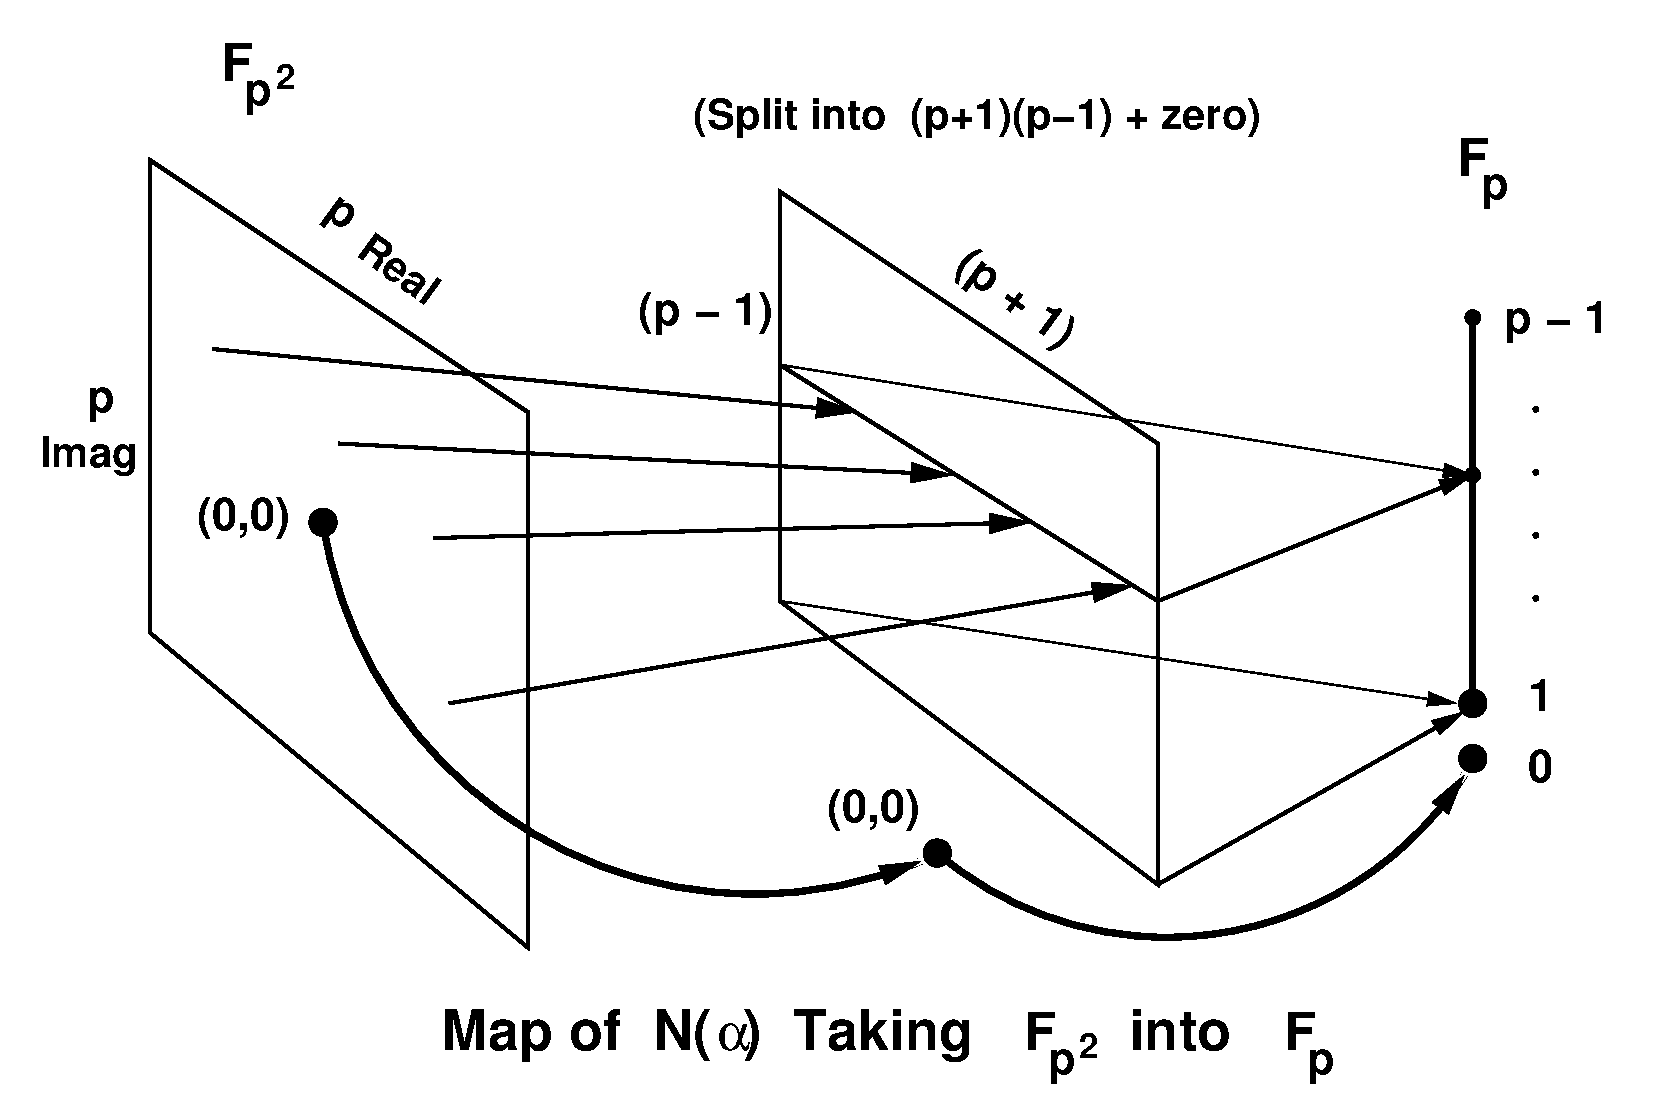
\includegraphics[width=3.6in]{Fpp2Fp}\caption{\label{proof1.fig}Sketch of the map from $\Fpp$ to $\Fp$ using
$\fnorm{\alpha}$, showing the decomposition of $\Fpp$ into the zero
element $\left(0,0\right)$ and the $p^{2}-1=\left(p+1\right)\left(p-1\right)$
non-zero elements that map onto the $p-1$ non-zero elements of $\Fp$
with multiplicity $p+1$.}
\end{figure}
We can now compute the size of the equivalence class of complex unit-modulus
phases corresponding to the Hopf fibration circle. %
\begin{comment}
\todo{Explain the Hopf fibration circle here\ldots ? }
\end{comment}
Since $\Fpp$ has $p^{2}-1$ non-zero values, and the map $\fnorm{\alpha}$
distributes these equally across the domain of $p-1$ non-zero elements
$c\in\Fp$, there are $\frac{p^{2}-1}{p-1}=p+1$ (non-zero) domain
elements in $\Fpp$ for each (non-zero) image element in $\Fp$. We
illustrate this graphically in Figure~\ref{proof1.fig}. Thus, the
Hopf circle always has the size $p+1$, corresponding essentially
to a discrete projective line, and that is the size of each equivalence
class of the map $\fnorm{\alpha}$ for non-vanishing $\alpha$, including
the map to the unit norm value $c=1\in\Fp$.\end{proof}

\subsection{Vector Spaces\label{subsec:Vector-Spaces}}

In this section, we want to build a theory of discrete vector spaces
that approximates as closely as possible the features of the conventional
quantum theory. Such a structure would ideally consist of the following:
(i) a vector space over the field of complex numbers, and (ii) an
inner product $\ip{\Phi}{\Psi}$ associating to each pair of vectors
a complex number, and satisfying the following properties:
\begin{enumerate}[label=(\Alph{enumi})]
\item \label{enu:inner-product-complex-conjugate}$\ip{\Phi}{\Psi}$ is
the complex conjugate of $\ip{\Psi}{\Phi}$;
\item \label{enu:inner-product-linear}$\ip{\Phi}{\Psi}$ is conjugate-linear
in its first argument and linear in its second argument;
\item \label{enu:inner-product-positive-definite}$\ip{\Psi}{\Psi}$ is
always non-negative and is equal to $0$ only if $\ket{\Psi}$ is
the zero vector.
\end{enumerate}
It turns out that a vector space defined over a finite field cannot
have an inner product satisfying the properties above. However, we
will introduce a Hermitian ``dot product'' satisfying some of those
properties.

We are interested in the vector space $\mathcal{H}$ of dimension
$D$ defined over the complexified field $\Fpp$. Let $\ket{\Psi}=\begin{pmatrix}\alpha_{0} & \alpha_{1} & \cdots & \alpha_{D-1}\end{pmatrix}^{T}$
and $\ket{\Phi}=\begin{pmatrix}\beta_{0} & \beta_{1} & \cdots & \beta_{D-1}\end{pmatrix}^{T}$
represent vectors in $\mathcal{H}$, with numbers $\alpha_{i}$ and
$\beta_{i}$ drawn from $\Fpp$, and where $\left(\cdot\right)^{T}$
is the transpose.

\begin{definition}[Hermitian dot product] Given vectors $\ket{\Phi}$
and $\ket{\Psi}\in\mathcal{H}$, it can be shown~\cite{grove2002classical,Wan2006}
the Hermitian dot product is always reducible to the form 
\begin{equation}
\ip{\Phi}{\Psi}=\sum_{i=0}^{D-1}\beta_{i}^{p}\alpha_{i}\,.\label{innerprod}
\end{equation}
If we use $\bra{\Phi}$ to represent the dual vector of $\ket{\Phi}$,
i.e., the conjugate transport of $\ket{\Phi}$, then the matrix multiplication
of $\bra{\Phi}$ and $\ket{\Phi}$ results a $1\times1$ matrix whose
only entry is their Hermitian dot product $\ip{\Phi}{\Psi}$.\end{definition}

Two vectors $\ket{\Phi}$ and $\ket{\Psi}\in\mathcal{H}$ are said
to be orthogonal if $\ip{\Phi}{\Psi}=0$. This product satisfies conditions~\ref{enu:inner-product-complex-conjugate}
and~\ref{enu:inner-product-linear} for inner products but violates
condition~\ref{enu:inner-product-positive-definite} since in every
finite field there always exists a non-zero vector $\ket{\Psi}$ such
that $\ip{\Psi}{\Psi}=0$. The reason is that addition in finite fields
eventually ``wraps around'' (because of their cyclic or modular
structure), allowing the sum of non-zero elements to be zero. The
fraction of non-zero vectors satisfying $\ip{\Psi}{\Psi}=0$ decreases
with the order $p$.

For any vector $\ket{\Psi}=\begin{pmatrix}\alpha_{0} & \alpha_{1} & \cdots & \alpha_{D-1}\end{pmatrix}^{T}$,
the Hermitian dot product $\ip{\Psi}{\Psi}$ is equal to $\sum_{i=0}^{D-1}\fnorm{\alpha_{i}}$,
which is the sum of the field norms for the complex coefficients.
For convenience, we now extend the field norm to include vector arguments
by defining 
\begin{equation}
\fnorm{\ket{\Psi}}=\ip{\Psi}{\Psi}=\sum_{i=0}^{D-1}\fnorm{\alpha_{i}}\,.\label{fnormD.eq}
\end{equation}

Although the field norm of a vector can vanish for non-vanishing vectors,
if a vector $\ket{\Psi}$ has a non-vanishing field norm~$c$, then
$\ket{\Psi}$ can be normalized by utilizing its field norm. Recalled
in Sec.~\ref{subsec:Complexified-Finite-Fields}, we defined $\fnorm*{\left\{ c\right\} }$
to be the set of elements whose field norm is $c$. Given any $\alpha\in\fnorm*{\left\{ c\right\} }$,
the field norm of $\frac{\ket{\Psi}}{\alpha}$ is
\begin{equation}
\fnorm{\frac{\ket{\Psi}}{\alpha}}=\frac{\fnorm{\ket{\Psi}}}{\fnorm{\alpha}}=\frac{c}{c}=1\,,
\end{equation}
i.e., $\frac{\ket{\Psi}}{\alpha}$ is normalized. However, since the
size of $\fnorm*{\left\{ c\right\} }$ is $p+1$, we cannot identify
a ``unique'' way to normalize any given vector.

The similar problem has already happened in conventional quantum theory.
For example, assume we want to normalize $\ket{\Psi}=\ket{0}+\ket{1}$.
Its inner product with itself is $\ip{\Psi}{\Psi}=2$. Since $\left(\pm\sqrt{2}\right)^{2}=2$,
both $\frac{\ket{\Psi}}{\sqrt{2}}$ and $\frac{\ket{\Psi}}{-\sqrt{2}}$
are normalized and representing the same state as $\ket{\Psi}$. In
this case, we systematically choose the state divided by the positive
square root as ``the'' normalized vector of $\ket{\Psi}$ in conventional
quantum theory, and the positive square root function is called the
\emph{principal} branch of $\sqrt{w}$~\cite{GAMELIN2003}. In the
discrete case, we can also systematically choose the \emph{principal
inverse field norm} by utilizing a generator $g\in\Fpp$ discussed
in Sec.~\ref{subsec:Complexified-Finite-Fields}. Because $g$ is
a generator, any non-zero element $c\in\ff{p}\backslash\left\{ 0\right\} $
can be expressed as $g^{\left(p+1\right)k}$ where $k$ is an integer
and $0\le k<p-1$, so we can define the principal inverse field norm
$\fnorm*{g^{\left(p+1\right)k}}$ as $g^{k}$. For example, the inverse
field norm over $\ff{3^{2}}$ with respect to the generator $1-\rmi$
is shown in Table~\ref{tab:Inverse-field-norm}. Given the non-normalized
state $\ket{\Psi}=\ket{0}+\ket{1}$, since its field norm is $\fnorm{\ket{\Psi}}=\fnorm{1}+\fnorm{1}=-1$,
it can be normalized as
\begin{equation}
\frac{\ket{\Psi}}{\fnorm*{-1}}=\frac{\ket{0}+\ket{1}}{1-\rmi}=\left(1+\rmi\right)\ket{0}+\left(1+\rmi\right)\ket{1}\,.
\end{equation}
\begin{table}
\begin{doublespace}
\noindent \centering{}\caption{\label{tab:Inverse-field-norm}Inverse field norm over $\ff{3^{2}}$
with respect to the generator $1-\rmi$}
\begin{tabular}{cccc}
\toprule 
$c=g^{\left(p+1\right)k}$ & $\left(p+1\right)k$ & $k$ & $\fnorm*{g^{\left(p+1\right)k}}=g^{k}$\tabularnewline
\midrule
$-1$ & $4$ & $1$ & $1-\rmi$\tabularnewline
$1$ & $0$ & $0$ & $1$\tabularnewline
\bottomrule
\end{tabular}
\end{doublespace}
\end{table}


\section{Irreducible Discrete $D$-dimensional States\label{DQCnqubitBloch.sec}}

In the one-qubit state with coefficients in $\Fpp$, the discrete
analog of the Bloch sphere is constructed by exact analogy to the
continuous case: we first require that the coefficients of the single
qubit basis obey 
\begin{equation}
\fnorm{\ket{\psi_{1}}}=\fnorm{\alpha_{0}}+\fnorm{\alpha_{1}}=1\label{DQA2.eq}
\end{equation}
in the discrete field. We show that there are $p\left(p^{2}-1\right)$
such values later in the general theorem, Proposition~\ref{appU.sec}.
Given this requirement, which is similar in form to the conservation
of probability, but not as useful due to the lack of orderable probability
values, we can immediately conclude that the discrete analog of the
Hopf fibration is again 
\begin{eqnarray}
X & = & 2\,\mathrm{Re}\ \alpha_{0}\alpha_{1}^{*}=2x_{0}x_{1}+2y_{0}y_{1}\,,\nonumber \\
Y & = & 2\,\mathrm{Im}\ \alpha_{0}\alpha_{1}^{*}=2x_{1}y_{0}-2x_{0}y_{1}\,,\label{DQA6.eq}\\
Z & = & \fnorm{\alpha_{0}}-\fnorm{\alpha_{1}}={x_{0}}^{2}+{y_{0}}^{2}-{x_{1}}^{2}-{y_{1}}^{2}\,,\nonumber 
\end{eqnarray}
but now with all computations in\hspace{0bp}$\pmod{p}$. At this
point, one can simply write down all possible discrete values for
the complex numbers $\left(\alpha_{0},\alpha_{1}\right)$ satisfying
Eq.~(\ref{DQA2.eq}) and enumerate those that project to the same
value of $\left(X,Y,Z\right)$. This equivalence class is the discrete
analog of the circle in the complex plane that was eliminated in the
continuous case. In Proposition~\ref{appH.sec}, we show that $p+1$
discrete values of $\left(\alpha_{0},\alpha_{1}\right)$ with unit
norm map to the same point under the Hopf map \Eq{DQA6.eq}; %
\begin{comment}
\todo{Does Proposition~\ref{appH.sec} really show this? }
\end{comment}
we may think of these as discrete circles or projective lines of equivalent,
physically indistinguishable, complex phase. The surviving $p\left(p-1\right)$
values of $\left(\alpha_{0},\alpha_{1}\right)$ correspond to irreducible
physical states of the discrete single qubit system. Thus, for example,
choosing the underlying field to be $\Fppx{3}$, there are exactly
6 single-qubit state vectors to populate the Bloch sphere; the four
equivalent phase-multiples mapping to each of the six points on the
$\Fppx{3}$ Bloch sphere are collapsed and regarded as physically
indistinguishable. In Figure~\ref{bloch.fig}, we plot the irreducible
states on the Bloch sphere for $p=3$, $7$, and $11$. Note that
the Cartesian lengths of the real vectors corresponding to the points
on the Bloch sphere vary considerably due to the nature of discrete
fields; we have artificially normalized them to a ``continuous world''
unit radius sphere for conceptual clarity.
\begin{figure}[!b]
\noindent \begin{centering}
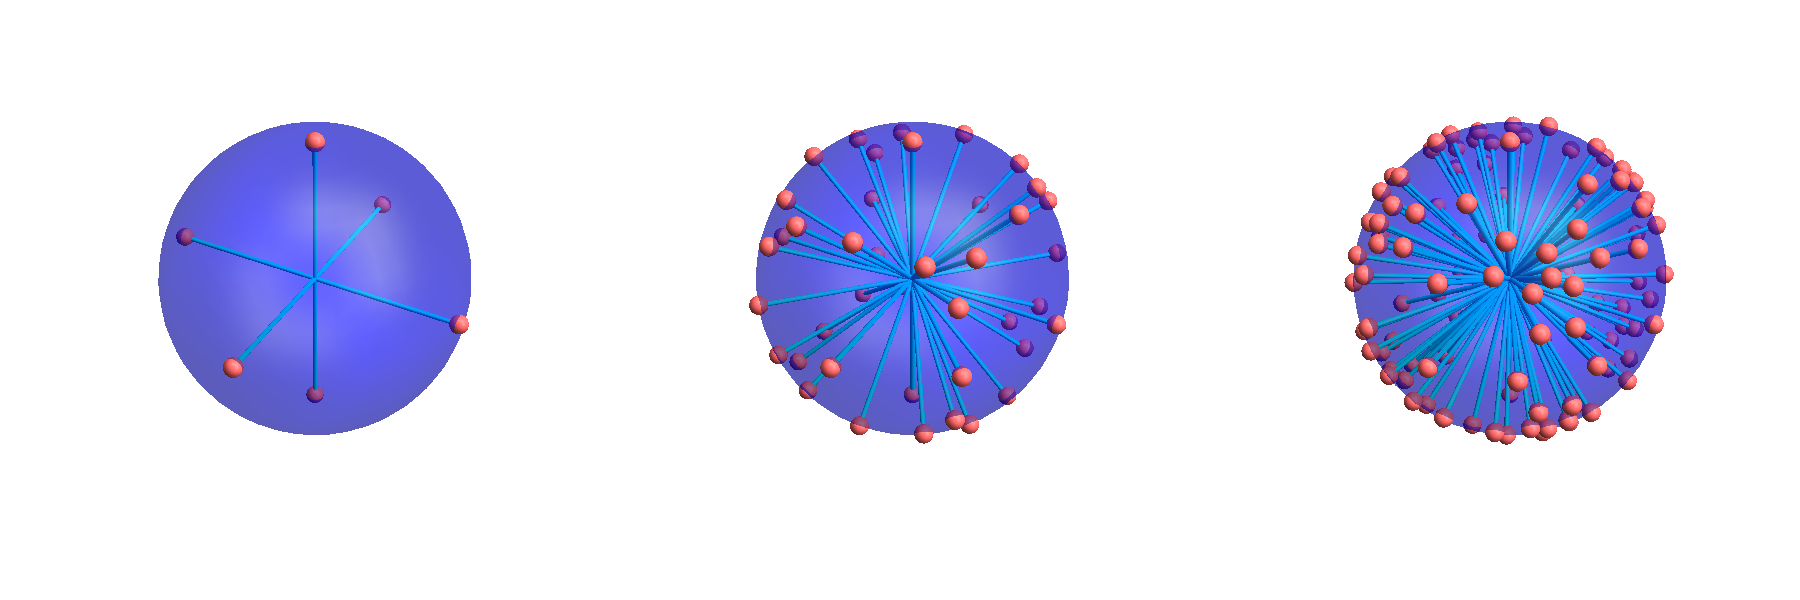
\includegraphics[viewport=200bp 0bp 1800bp 600bp,width=1.1\columnwidth]{picC}
\par\end{centering}
\caption{\label{bloch.fig}Schematically normalized plots of the elements of
the discrete Bloch sphere, the irreducible single-qubit (two-dimensional)
state vectors with unit norm over the field $\Fpp$. We show the results
for $p=3$, $7$, and $11$. For example, in $\Fppx{3}$, there are
24 vectors of unit norm, but only the 6 inequivalent classes appear
in the plot. The $p+1=4$ equivalent vectors in each class differ
only by a complex discrete phase.}
\end{figure}


\subsection{Counting states on the discrete Bloch sphere}

We have the unique opportunity in the finite-field approach to quantum
computing to precisely identify and enumerate the physical states.
In the conventional theory, as we have seen in Sec.~\ref{subsec:Explicit-generalization-of},
we employ a generalized Hopf fibration on the normalized states to
project out a circle of phase-equivalent states, yielding the generalized
Bloch sphere.

In the introduction to this subsection, we sketched the counting of
the irreducible single-qubit discrete states. To count the number
of inequivalent discrete states for the general $n$-qubit case with
coefficients in $\Fpp$, we first must find the set of unit-norm states,
and then determine the equivalence classes of unit-norm states under
discrete phase transformations; we can then enumerate the list of
states on the discrete generalized Bloch sphere. By executing computer
searches of these spaces, we discovered a hypothesis for a closed-form
solution for the counting of the states and found a rigorous proof
of the enumeration.

This process of describing the discrete $D$-dimensional irreducible
states can again be understood geometrically by following the discrete
analog of the Hopf fibration. First, we construct the discrete version
of the quadratic unit-length form that automatically annihilates the
distinction among states differing only by a discrete phase, 
\begin{equation}
\Hat{a}=\left(\fnorm{\alpha_{i}},\ldots,\sqrt{2}\,\mathrm{Re}\ \alpha_{i}\alpha_{j}^{*},\ldots,\sqrt{2}\,\mathrm{Im}\ \alpha_{i}\alpha_{j}^{*},\ldots\right)\,,
\end{equation}
where 
\begin{equation}
\Hat{a}\cdot\Hat{a}=\left(\sum_{i=0}^{D-1}\fnorm{\alpha_{i}}\right)^{2}=1\,.
\end{equation}
From Proposition~\ref{appH.sec}, we know that $p+1$ elements of
this discrete $\Sphere{2D-1}$ structure map to the \textit{same point}
in $\Hat{a}$. %
\begin{comment}
\todo{Does Proposition~\ref{appH.sec} really show this? }
\end{comment}
Each set of $p+1$ redundant points is, geometrically speaking, the
\textit{discrete Hopf fibration circle} living above each \textit{irreducible}
point of the $D$-dimensional state description. These $p+1$ points
are interpretable as the $p$ finite points plus the single point
at infinity of the projective discrete line (see, e.g.,~\cite{arnold_2010}).

The next part of this argument is the determination of the unit-norm
states, effectively the space of allowed discrete partitions of unity;
we cannot exactly call these ``probability-conserving'' sectors
of the state coefficients since we do not have a well-defined notion
of probability, but we do have a well-defined notion of the partition
of unity. Compared to the total number $p^{2D}$ of possible complex
integer state vectors that could be chosen, the number of unit-norm
states is given by the following proposition. This unit-norm state
structure is the discrete analog of $\Sphere{2D-1}$.

\begin{prop}\label{appU.sec}The number of unit-norm states described
by a $D$-dimensional vector $(\alpha_{0},\ldots,\alpha_{D-1})$ with
coefficients $\alpha_{i}\in\Fpp$ is $p^{D-1}\left(p^{D}-\left(-1\right)^{D}\right)$.\end{prop}

\begin{proof}Proposition~11.27 in Grove~\cite{grove2002classical}
provides the count of the zero-norm states $\zeta\left(D,p\right)=p^{D-1}\left(p^{D}+\left(-1\right)^{D}\left(p-1\right)\right)$.
Since there are $p^{2}$ elements $\alpha\in\Fpp$, we must have $\left(p^{2}\right)^{D}=p^{2D}$
possible values of a $D$-dimensional vector $(\alpha_{0},\ldots,\alpha_{D-1})$.
There are $p^{2}-1$ non-zero values of $\alpha\in\Fpp$, and we showed
in Proposition~\ref{appH.sec} that $\fnorm{\alpha}$ maps exactly
$p+1$ values in that set to each of the $p-1$ non-zero values in
$\Fp$. Therefore, the \textit{unit-norm case} has a count of domain
elements that is $\frac{1}{p-1}$ of the total number of non-zero-norm
cases, 
\begin{equation}
\frac{p^{2D}-\zeta\left(D,p\right)}{p-1}=\frac{p^{2D}-p^{2D-1}-\left(-1\right)^{D}p^{D-1}\left(p-1\right)}{p-1}=p^{D-1}\left(p^{D}-\left(-1\right)^{D}\right)\,.\label{unitnorm.eq}
\end{equation}
\end{proof}

Finally, we repeat the last step of the $D$-dimensional continuous
Hopf fibration process for discrete $D$-dimensional states, eliminating
the discrete set of $p+1$ equivalent points that map to the same
point $\Hat{a}$ on the generalized Bloch sphere. Dividing the tally
$p^{D-1}\left(p^{D}-\left(-1\right)^{D}\right)$ of unit norm states
by the $p+1$ elements of each phase-equivalent discrete circle, we
find
\begin{equation}
\frac{p^{D-1}\left(p^{D}-\left(-1\right)^{D}\right)}{p+1}\label{eq:numberOfIrreducibleStates}
\end{equation}
as the total count of unique irreducible states in a discrete $D$-dimensional
configuration. The resulting object is precisely the discrete version
of $\CP{D-1}$, which we might call a \textit{discrete complex projective
space} or $\DCP{D-1}$.

\section{Geometry of Entangled States\label{sec:Geometry-of-Entangled-States}}

To discuss entanglement, we consider a $D$-dimensional quantum system
composed of $n$-qubit subsystems, i.e., $D=2^{n}$ as usual. Without
regard to uniqueness, an $n$-qubit state with discrete complex coefficients
in $\Fpp$ will have the total possible space of coefficients with
dimension $p^{2\times2^{n}}$ (including the null state). Imposing
the condition of a length-one norm in $\Fp$, this number is reduced
to $p^{2^{n}-1}\left(p^{2^{n}}-1\right)$. The ratio of all the states
to the unit-norm states is asymptotically $p$: 
\begin{equation}
\frac{p^{2^{n}+1}}{p^{2^{n}}-1}\rightarrow p\,,
\end{equation}
so there are roughly $p$ sets of coefficients, for any number of
qubits $n$, that are discarded for each retained unit-length state
vector. A factor of $p+1$ more states is discarded in forming the
discrete Bloch sphere of irreducible states. Selected plots of the
full space compared to both the unit-norm space and the irreducible
space for a selection of complexified finite fields are shown in Figure~\ref{statePlot3Unit.fig}
for 1, 2, 3, and 4 qubits.
\begin{figure}[!b]
\begin{centering}
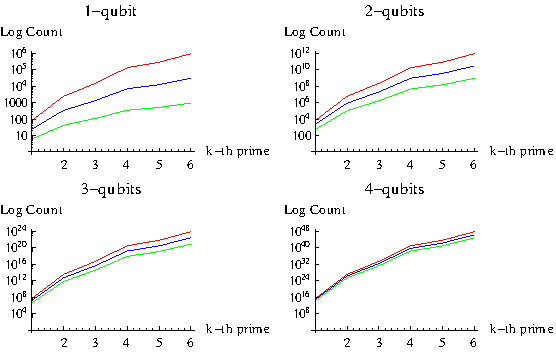
\includegraphics[width=1\columnwidth]{statePlot3}
\par\end{centering}
\caption{\label{statePlot3Unit.fig}Logarithmic plot of the number of discrete
unnormalized states (top, in red), vs the number of normalized discrete
states (middle, in blue), vs the irreducible states (bottom, in green)
for the first 6 $\Fpp$-compatible primes, ($3$, $7$, $11$, $19$,
$23$, $31$), for the number of qubits $1$, $2$, $3$, and $4$.}
\end{figure}


\subsection{Unentangled vs Entangled Discrete States}

For a given $p$ and the corresponding complexified field $\Fpp$,
the $n$-qubit discrete quantum states with coefficients in $\Fpp$
can be classified by their degree of entanglement to a level of precision
that is unavailable in the continuous theory. We look first at the
unentangled $n$-qubit states, which are direct product states of
the form 
\begin{equation}
\ket{\Psi}=\ket{\psi_{1}}\otimes\cdots\otimes\ket{\psi_{j}}\otimes\cdots\otimes\ket{\psi_{n}}\,.\label{dqcNqUntg.eq}
\end{equation}
Without regard to normalization, there are $\left(p^{4}\right)^{n}$
possible unentangled states out of the total of $p^{2\times2^{n}}$
states noted above. When we normalize the individual product states
to unit norm, the norm of the entire $n$-qubit state becomes the
product of those unit norms and is automatically normalized to one.
We have already seen that each single-qubit normalized state in the
tensor product Eq.~(\ref{dqcNqUntg.eq}) has precisely $p\left(p-1\right)$
irreducible components due to $D=2$ case in Eq.~(\ref{eq:numberOfIrreducibleStates}).

\subsection{Completely Unentangled States and the Discrete Bloch Sphere}

In effect, the irreducible states for unentangled $n$-qubit configurations
reduce to a single Bloch sphere for each one-qubit component $\ket{\psi_{j}}$,
and thus the whole set of states is defined by an $n$-tuple of discrete
Bloch sphere coordinates. Since each Bloch sphere in $\Fpp$ has $p\left(p-1\right)$
distinct irreducible components, we have 
\begin{equation}
\mbox{{\bf Count of Unentangled States}}=p^{n}\left(p-1\right)^{n}\,.\label{eq:CountUnentangledStates}
\end{equation}

According to Eq.~(\ref{eq:numberOfIrreducibleStates}), we know that
the total number of irreducible states (points in the generalized
$\DCP{2^{n}-1}$ Bloch sphere) for an $n$-qubit state is $\frac{p^{2^{n}-1}\left(p^{2^{n}}-1\right)}{p+1}$,
and so the number of states containing some measure of entanglement
is 
\begin{equation}
\mbox{{\bf Count of Entangled States}}=\frac{p^{2^{n}-1}\left(p^{2^{n}}-1\right)}{p+1}-p^{n}\left(p-1\right)^{n}\,.
\end{equation}
Therefore, a very small fraction of the unit norm states is unentangled.

\subsection{Maximal entanglement\label{subsec:Maximal-entanglement}}

Equation~(\ref{purityMeasure.eq}) for $P_{\fh}$ includes a normalization
factor~$\frac{1}{n}$. In the discrete case, this normalization factor
is undefined when $p\mid n$. Equation~(\ref{purityMeasure.eq})
also includes a summation of $n$ terms. In the discrete case, certainly
when $p\mid n$ but also in other cases, this summation may vanish
in the field even if the individual summands are non-zero. These anomalies
are irrelevant for the classification of unentangled states as this
computation is performed by directly checking the possibility of direct
decomposition into product states, disregarding equation~(\ref{purityMeasure.eq}).

For maximally entangled states, the purity calculation in conventional
quantum mechanics using equation~(\ref{purityMeasure.eq}) produces
0. Given the above observations, in a discrete field, equation~(\ref{purityMeasure.eq})
may be undefined or may report a purity of 0 even for partially entangled
states. For example, the normalized 5-qubit state $\ket{\Psi}=\left(1-\rmi\right)\left(\ket{00}+\ket{11}\right)\otimes\ket{000}$
has $P_{\fh}=0$ for $p=3$, and is not maximally entangled because
only the first two qubits are entangled. In the discrete case, we
therefore check for maximally entangled states using the following
equations~\cite{Gardiner2014}, 
\begin{equation}
\forall j,\forall\eta\in\left\{ x,y,z\right\} ,\expval{\jthSubsystem{\sigma}[\eta]{j}}^{2}=0\textrm{ ,}\label{eq:john}
\end{equation}
which avoids the normalization factor and simply checks that each
summand is 0, where $\expval{\jthSubsystem{\sigma}[\eta]{j}}$ is
defined as $\melem{\Psi}{\jthSubsystem{\sigma}[\eta]{j}}{\Psi}$.

We now implement these procedures to enumerate the maximally entangled
states for the specific cases for $n=2,3$ and compare these to the
counts for product states. We have verified explicitly in Eq.~(\ref{eq:CountUnentangledStates})
that the numbers of unit-norm product states for $n=2$, $p=\{3,7,11,19,\ldots\}$
are 
\begin{equation}
(p+1)p^{2}(p-1)^{2}=\{144,14112,145200,2339280,\ldots\}\,,
\end{equation}
and for general $n$, $(p+1)p^{n}(p-1)^{n}$. The irreducible state
counts are reduced by $(p+1)$, giving 
\begin{equation}
p^{2}(p-1)^{2}=\{36,1764,12100,116964,\ldots\}\,,
\end{equation}
and in general for $n$-qubits, there are $p^{n}\left(p-1\right)^{n}$
instances of pure product states.

Performing the computation using equation (\ref{eq:john}), we find
the numbers of maximally entangled states for two qubits to be 
\begin{equation}
p\left(p^{2}-1\right)\left(p+1\right)=\left\{ 96,2688,15840,136800,\ldots\right\} \,.
\end{equation}
The irreducible state counts for maximal entanglement are reduced
by $\left(p+1\right)$, giving, for $n=2$, 
\begin{equation}
p\left(p^{2}-1\right)=\left\{ 24,336,1320,6840,\ldots\right\} \,.
\end{equation}
For three qubits, there are $p^{3}\left(p^{4}-1\right)\left(p+1\right)$
(total) and $p^{3}\left(p^{4}-1\right)$ (irreducible) instances of
pure maximally entangled states. For four-qubits and $p=3$, there
are $2195538048$ instances of pure maximally entangled states, while
the general formula for four-qubit states remains unclear.

Therefore, the ratio of maximally entangled to product states is 
\begin{equation}
\frac{\textbf{Max entangled}}{\textbf{Product}}=\frac{p+1}{p\left(p-1\right)}\textrm{ and }\frac{\left(p^{2}+1\right)\left(p+1\right)}{\left(p-1\right)^{2}}
\end{equation}
for $n=2$ and $3$, respectively.

\section{Discrete Quantum Computing (I)\label{discretequantumcomputingI}}

Given a complexified finite field $\ff{p^{2}}$ and its Hermitian
\dotprod\  (Eq.~\eqref{innerprod}) much of the structure of conventional
quantum computing can be recovered. For example, the smallest field~$\ff{3^{2}}$
is already rich enough to express the standard Deutsch-Jozsa algorithm
\cite{DeutschJozsa1992,544199,Jaeger2007}, which requires only normalized
versions of vectors or matrices with the scalars $0$, $1$, and $-1$.
Similarly, other deterministic quantum algorithms (algorithms for
which we may determine the outcome with certainty), such as Simon's
\cite{Simon:1994:PQC:1398518.1399019,Mermin2007,Jaeger2007} and Bernstein-Vazirani
\cite{Bernstein:1993:QCT:167088.167097,Mermin2007}, perform as desired.
In the following subsection, we will present the discrete Deutsch
algorithm as an example. However, this quantum computing model is
still different from the conventional one. On one hand, algorithms
such as Grover's search \cite{Grover:1996:FQM:237814.237866,Mermin2007,Jaeger2007}
will not work in the usual way because we lack (the notion of) ordered
angles and probability in general. On the other hand, this computational
model still leads to excessive computational power for the unstructured
database search problem for certain database sizes. %
\begin{comment}
\todo{Prof.~Gil~Kalai thought it would be interesting if we can
do Simon's algorithm in DQC~(I), but I don't know when I could organize
my unreadable draft to a readable one\ldots{} Moreover, Prof.~Ortiz
wants to check Shor's algorithm in DQC~(I).}
\end{comment}


\subsection{Discrete Deutsch algorithm\label{subsec:Discrete-Deutsch-algorithm}}

\begin{table}
\begin{doublespace}
\noindent \centering{}\caption{\label{tab:Possible-f}All Possible $f\colon\boolt\rightarrow\boolt$.}
\begin{tabular}{ccccc}
\toprule 
$x$ & $f_{1}\left(x\right)$ & $f_{2}\left(x\right)$ & $f_{3}\left(x\right)$ & $f_{4}\left(x\right)$\tabularnewline
\midrule
$\bfalse$ & $\bfalse$ & $\bfalse$ & $\btrue$ & $\btrue$\tabularnewline
$\btrue$ & $\bfalse$ & $\btrue$ & $\bfalse$ & $\btrue$\tabularnewline
\midrule 
constant or balanced? & constant & balanced & balanced & constant\tabularnewline
\bottomrule
\end{tabular}
\end{doublespace}
\end{table}
\begin{comment}
\todo{We typeset $U_{f}$ either directly or use macro \textbackslash uf,
but the definition of \textbackslash uf has a negative space between
$U$ and $f$ which is different from U\_\{f\}\ldots{} I need to understand
whether the negative space is necessary or not, or whether the negative
space has any semantic meaning\ldots{} }
\end{comment}
Although having no realistic application, the Deutsch algorithm is
the first quantum algorithm which outperforms any possible classical
algorithm for the Deutsch problem \cite{Deutsch1985,544199,Mermin2007}.
The Deutsch problem is to decide whether a function $f\colon\boolt\rightarrow\boolt$
is constant or balanced. As listed in Table~\ref{tab:Possible-f},
we have only $4$ different $f$: $2$ of them are constant while
another $2$ are balanced. Similar to our $\usat$ algorithm in Sec.~\ref{modalquantumcomputing},
we start by representing $f$ as a Deutsch black box $U_{f}$ in the
middle of the quantum circuit, Figure~\ref{fig:Quantum-Circuit-Deutsch}.
To explain why this circuit solves the Deutsch problem, we then compute
the state in each step explicitly and express them in the Dirac bracket
notation and its matrix representation in the computational basis
$\left\{ \ket{00},\ket{01},\ket{10},\ket{11}\right\} $.
\begin{figure}[!b]
\noindent \centering{}
\[
\begin{array}{c}
\xyR{.9em}\xyC{.6em}\entrymodifiers={@*=<0em>}\xymatrix{ & \ar@{.}[ddd] &  & \ar@{.}[ddd] &  & \ar@{.}[ddd] &  & \ar@{.}[ddd]\\
\lstick{\ket{1}} & \qw & \gate{H} & \qw & \multigate{1}{\uf} & \qw & \gate{H^{\dagger}} & \qw & \multimeasureD{1}{\text{measure}}\\
\lstick{\ket{0}} & \qw & \gate{H} & \qw & \ghost{\uf} & \qw & \gate{H^{\dagger}} & \qw & \ghost{\text{measure}}\\
 & \push{\ket{\Phi_{1}}} &  & \push{\ket{\Phi_{2}}} &  & \push{\ket{\Phi_{3}}} &  & \push{\ket{\Phi_{4}}}
}
\end{array}
\]
\caption{\label{fig:Quantum-Circuit-Deutsch}Quantum Circuit for the Deutsch
Algorithm.}
\end{figure}

First, a 2-qubit pure state is initialized to $\ket{\Phi_{1}}=\ket{1}\ket{0}=\left(\begin{smallmatrix}0\\
1
\end{smallmatrix}\right)\otimes\left(\begin{smallmatrix}1\\
0
\end{smallmatrix}\right)$.

Second, on both initialized qubits, we apply the Hadamard matrix $H=\frac{1}{\alpha}\left(\begin{smallmatrix}1 & 1\\
1 & -1
\end{smallmatrix}\right)$ over $\Fpp$, where $\alpha=\fnorm*{2}$ is the principal inverse
field norm which is used to replace the square root $\sqrt{2}$ in
the conventional Hadamard matrix $\frac{1}{\sqrt{2}}\left(\begin{smallmatrix}1 & 1\\
1 & -1
\end{smallmatrix}\right)$ as discussed in Sec.~\ref{subsec:Vector-Spaces}. The second step
produces
\[
\ket{\Phi_{2}}=\left(H\otimes H\right)\ket{\Phi_{1}}=\left[\frac{1}{\alpha}\begin{pmatrix}1 & 1\\
1 & -1
\end{pmatrix}\begin{pmatrix}0\\
1
\end{pmatrix}\right]\otimes\left[\frac{1}{\alpha}\begin{pmatrix}1 & 1\\
1 & -1
\end{pmatrix}\begin{pmatrix}1\\
0
\end{pmatrix}\right]=\ket{-}\ket{+}\,,
\]
where
\begin{align}
\ket{+} & =\frac{1}{\alpha}\begin{pmatrix}1\\
1
\end{pmatrix}=\frac{\ket{0}+\ket{1}}{\alpha}\,, & \ket{-} & =\frac{1}{\alpha}\begin{pmatrix}1\\
-1
\end{pmatrix}=\frac{\ket{0}-\ket{1}}{\alpha}\,.
\end{align}

Third, the Deutsch black box~$U_{f}$ is applied to the state $\ket{\Phi_{2}}$.
According to Eq.~(\ref{eq:DeutschBox}), these Deutsch black box
will be used to apply exclusive disjunction on the first qubit, where
we respectively identify $\bfalse$ and $\btrue$ as $0$ and $1$
as usual. Since our first qubit is $\ket{-}$, the value $f\left(x\right)$
could be moved outside as a phase no matter $f\left(x\right)$ is
$\bfalse$ or $\btrue$:
\begin{equation}
\begin{aligned}U_{f}\ket{-}\ket{x} & =\tfrac{1}{\alpha}\left[\ket{0\oplus f\left(x\right)}\ket{x}-\ket{1\oplus f\left(x\right)}\ket{x}\right]\\
 & =\begin{cases}
\frac{1}{\alpha}\left[\ket{0}\ket{x}-\ket{1}\ket{x}\right] & \textrm{if }f\left(x\right)=\bfalse=0\,;\\
\frac{1}{\alpha}\left[\ket{1}\ket{x}-\ket{0}\ket{x}\right] & \textrm{if }f\left(x\right)=\btrue=1
\end{cases}\\
 & =\left(-1\right)^{f\left(x\right)}\ket{-}\ket{x}\,.
\end{aligned}
\end{equation}
Then, $\ket{\Phi_{3}}$ can be evaluated as follow:
\begin{equation}
\begin{aligned}\ket{\Phi_{3}} & =U_{f}\ket{-}\ket{+}=\tfrac{1}{\alpha}\left[U_{f}\ket{-}\ket{0}+U_{f}\ket{-}\ket{1}\right]\\
 & =\tfrac{1}{\alpha}\left[\left(-1\right)^{f\left(0\right)}\ket{-}\ket{0}+\left(-1\right)^{f\left(1\right)}\ket{-}\ket{1}\right]\\
 & =\begin{cases}
\left(-1\right)^{f\left(0\right)}\ket{-}\ket{+} & \textrm{if }f\left(0\right)=f\left(1\right)\,;\\
\left(-1\right)^{f\left(0\right)}\ket{-}\ket{-} & \textrm{if }f\left(0\right)\ne f\left(1\right)\,.
\end{cases}
\end{aligned}
\end{equation}

Finally, $\ket{\Phi_{4}}$ can then be obtained by applying the Hermitian
conjugate of Hadamard matrix $H^{\dagger}=\frac{1}{\alpha^{*}}\left(\begin{smallmatrix}1 & 1\\
1 & -1
\end{smallmatrix}\right)$ on both qubits. If $f\left(0\right)=f\left(1\right)$, i.e., $f$
is constant, we have 
\[
\ket{\Phi_{4}}=\left(-1\right)^{f\left(0\right)}\left[\dfrac{1}{\alpha^{*}}\begin{pmatrix}1 & 1\\
1 & -1
\end{pmatrix}\frac{1}{\alpha}\begin{pmatrix}1\\
-1
\end{pmatrix}\right]\otimes\left[\dfrac{1}{\alpha^{*}}\begin{pmatrix}1 & 1\\
1 & -1
\end{pmatrix}\frac{1}{\alpha}\begin{pmatrix}1\\
1
\end{pmatrix}\right]=\left(-1\right)^{f\left(0\right)}\ket{1}\ket{0}\,;
\]
if $f\left(0\right)\ne f\left(1\right)$, i.e., $f$ is balanced,
we have 
\[
\ket{\Phi_{4}}=\left(-1\right)^{f\left(0\right)}\left[\dfrac{1}{\alpha^{*}}\begin{pmatrix}1 & 1\\
1 & -1
\end{pmatrix}\frac{1}{\alpha}\begin{pmatrix}1\\
-1
\end{pmatrix}\right]\otimes\left[\dfrac{1}{\alpha^{*}}\begin{pmatrix}1 & 1\\
1 & -1
\end{pmatrix}\frac{1}{\alpha}\begin{pmatrix}1\\
-1
\end{pmatrix}\right]=\left(-1\right)^{f\left(0\right)}\ket{1}\ket{1}\,.
\]
Hence, we can decide whether $f$ is constant or balanced by measuring
$\ket{\Phi_{4}}$ in the computational basis.

\subsection{Partial \usat\ Algorithm\label{subsec:Partial-Algorithm}}

\begin{figure}[!b]
\centering{}
\[
\xyR{.9em}\xyC{.6em}\entrymodifiers={@*=<0em>}\xymatrix{\lstick{y=\ket{0}} & \qw & \multigate{3}{\uf} & \qw & \multimeasureD{3}{\text{measure}}\\
\lstick{x_{1}=\ket{0}} & \multigate{2}{\otimes H} & \ghost{\uf} & \multigate{2}{\otimes H^{\dagger}} & \ghost{\text{measure}}\\
\lstick{\ldots} & \ghost{\otimes H} & \ghost{\uf} & \ghost{\otimes H^{\dagger}} & \ghost{\text{measure}}\\
\lstick{x_{n}=\ket{0}} & \ghost{\otimes H} & \ghost{\uf} & \ghost{\otimes H^{\dagger}} & \ghost{\text{measure}}
}
\]
\caption{\label{fig:dbsearch}Circuit for the black box \usat\ in discrete
quantum computing.}
\end{figure}
It is possible, in some situations, to exploit the cyclic behavior
of the field to creatively cancel probability amplitudes and solve
problems with what again appears to be ``supernatural'' efficiency.
We illustrate this behavior with the algorithm in Fig.~\ref{fig:dbsearch},
which is a variant of the one in Fig.~\ref{fig:alg}. Unlike the
modal quantum algorithm, the new algorithm does not always succeed
deterministically using a constant number of black box evaluations.
We can, however, show that supernatural behavior occurs if the characteristic
$p$ of the field divides $2^{N}-1$. For a database of fixed size
$N$, matching the conditions becomes less likely as the size of the
field increases. Nevertheless, for a \textit{given} field, it is always
possible to expand any database with dummy records to satisfy the
divisibility property. Physically, we are taking advantage of additional
interference processes that happen because of the possibility of ``wrapping
around'' due to modular arithmetic. We do not know, in general, whether
this version of discrete quantum computing actually enables the rapid
solution of $\NP$-complete problems.

\section{Discrete Quantum Theory (II)\label{sec:Discrete-Quantum-Theory-(II)}}

\subsection{Inner Product Space\label{discretequantumtheoryIIa}}

We next discuss an approach using finite complexifiable fields that
conditionally resolves the inner product condition~\ref{enu:inner-product-positive-definite}
discussed in Sec.~\ref{subsec:Vector-Spaces}, which is violated
by the theory just presented. A possible path is suggested by the
work of Reisler and Smith~\cite{ReislerSmith1969}. The general idea
is that while the cyclic properties of arithmetic in finite fields
make it impossible to \emph{globally} obtain the desired properties
of the conventional Hilbert space inner product, it \textit{is} possible
to recover them \emph{locally}, thereby restoring, with some restrictions,
all the usual properties of the inner product needed for conventional
quantum mechanics and conventional quantum computing. As the size
of the discrete field becomes large, the size of the locally valid
computational framework grows as well, leading to the \emph{effective
emergence of conventional quantum theory}. We next briefly outline
such a context for local orderable subspaces of a finite field and
introduce an improvement on the original method~\cite{ReislerSmith1969}
suggested by recent number theory resources~\cite{Sloane2005}.

Let us first note that the range of the quadratic map, $\set{x^{2}\bmod p}{x\in\ff{p}}$,
is always one-half of the non-zero elements of $\ff{p}$, and is the
set of elements with square roots in the field. This is the set of
\emph{quadratic residues}, and the complementary set (the other half
of the non-zero field elements) is the set of \emph{quadratic non-residues}.
For example in $\ff{7}$, the elements $\left\{ 1,2,4\right\} $ are
considered positive as they have the square roots $\left\{ 1,3,2\right\} $
respectively; the remaining elements $\left\{ 3,5,6\right\} $ do
not have square roots in the field. What is interesting is that if
we have an uninterrupted sequence of numbers that are all quadratic
residues, then we can define a \textit{transitive order}, with $a>c$
if $a>b$ and $b>c$, provided $a-b$, $b-c$, and $a-c$ are all
quadratic residues. %
\begin{comment}
\todo{Should we remove the quadratic residue part? Since we never
use take the square roots of numbers in order range later, whether
they are the quadratic residues or not doesn't really matter\ldots}
\end{comment}

As a concrete example, consider a finite field in which the sequential
elements $0$, $1$, $2$, $3$, \ldots , and $k-1$ are all quadratic
residues (including $0$). Then any sequence of odd length~$k$ and
centered around an arbitrary $x\in\ff{p}$, i.e., $S_{x}\left(k\right)=x-\frac{k-1}{2}$,
\ldots , $x-2$, $x-1$, $x$, $x+1$, $x+2$, \ldots , $x+\frac{k-1}{2}$,
is \textit{transitively ordered}. Indeed, we have $\left(x+1\right)-x=1$
which is a quadratic residue and hence $x+1>x$. Similarly, $x-\left(x-1\right)=1$
and hence $x>x-1$. Also, $\left(x+1\right)-\left(x-1\right)=2$ which
is a quadratic residue and hence $x+1>x-1$. Clearly, this process
may be continued to show that the sequence $S_{x}\left(k\right)$
is transitively ordered. We can construct examples using the sequence
A000229 in the encyclopedia of integer sequences~\cite{Sloane2005}.\footnote{For computational purposes, this sequence is preferable to the one
proposed by Reisler and Smith~\cite{ReislerSmith1969} because it
produces smaller primes. Their work showed that a sufficient condition
on finite fields to produce sequences of quadratic residues is to
further constrain the underlying prime numbers to be of the form $8\prod_{i=1}^{m}q_{i}-1$,
where $q_{i}$ is the $i$-th odd prime. While all such primes are
of the form $4\ell+3$, the set is severely restricted to astronomical
numbers because the first few such primes are $7$, $23$, $839$,
$9239$, $2042039$, \ldots} The $n$-th element of that sequence (which must be prime) is the
least number such that the $n$-th prime is the \emph{least} quadratic
non-residue for the given element. The first few elements of this
sequence are listed in the top row of Table~\ref{pseq}. The next
row lists the number $k$ of transitively ordered consecutive elements
in that field, and $\pi\left(k\right)$ in the bottom row is the prime
counting function (the number of primes up to $k$).
\begin{table}
\begin{doublespace}
\noindent \centering{}\caption{\label{pseq}Number $k$ of transitively ordered elements for a given
field $\ff{p}$.}
\begin{tabular}{cccccccccccc}
\toprule 
$p$ & $3$ & $7$ & $23$ & $71$ & $311$ & $479$ & $1559$ & $5711$ & $10559$ & $18191$ & $\cdots$\tabularnewline
\midrule 
$k$ & ${\bf 2}$ & ${\bf 3}$ & ${\bf 5}$ & ${\bf 7}$ & ${\bf 11}$ & ${\bf 13}$ & ${\bf 17}$ & ${\bf 19}$ & ${\bf 23}$ & ${\bf 29}$ & $\cdots$\tabularnewline
\midrule
$\pi\left(k\right)$ & $1$ & $2$ & $3$ & $4$ & $5$ & $6$ & $7$ & $8$ & $9$ & $10$ & $\cdots$\tabularnewline
\bottomrule
\end{tabular}
\end{doublespace}
\end{table}

As an example, consider the field $\ff{23}$. Looking at the squares
of the numbers $\ff{23}=\{0,\ldots,22\}$ modulo 23, we find the $2$-centered
uninterrupted sequence $S_{2}\left(5\right)=\{0,1,2,3,4\}$, followed
by $5$, which is both the smallest quadratic non-residue and the
size of the uninterrupted sequence of quadratic residues (including
$0$) of interest. In particular, it is possible to construct a total
order for the elements $S_{0}\left(5\right)=\{-2,-1,0,1,2\}$ in the
fields $\ff{23}$, $\ff{71}$, $\ff{311}$, etc., but not in the smaller
fields $\ff{3}$ and $\ff{7}$.

Given a $D$-dimensional vector space over $\ff{p^{2}}$ where~$p$
is one of the primes above, it is possible to define a \emph{region}
over which an inner product and norm can be identified. Let the length
of the sequence of quadratic residues be $k$. The region of interest
includes all vectors $\ket{\Psi}=\sum_{i=0}^{D-1}\alpha_{i}\ket{i}=\begin{pmatrix}\alpha_{0} & \alpha_{1} & \cdots & \alpha_{D-1}\end{pmatrix}^{T}$,
for which $D<p-\frac{k-1}{2}$ and each $\alpha_{i}$ satisfies 
\begin{equation}
D\,\fnorm{\alpha_{i}}=D\,\left(a_{i}^{2}+b_{i}^{2}\right)\leq\frac{k-1}{2}\,,\label{eq:region}
\end{equation}
with $a_{i}$ and $b_{i}$ drawn from the set $S_{0}\left(k\right)$.
Consider, for example, $\ff{311^{2}}$ ($p=311$, $k=11$). We find
that we can trade off the dimension $D$ of the vector space against
the range of probability amplitudes available for each $\alpha_{i}$
in Table~\ref{table_allowed}.
\begin{table}
\begin{doublespace}
\noindent \centering{}\caption{\label{table_allowed}Allowed probability amplitudes for different
vector space dimensions $D$ and $k=11$.}
\begin{tabular}{ll}
\toprule 
 & allowed probability amplitudes $F^{D}\left(k\right)$ \tabularnewline
\midrule
$D=1$  & $F^{1}\left(11\right)=\left\{ 0,\pm1,\pm2,\pm\rmi,\pm2\rmi,(\pm1\pm\rmi),(\pm1\pm2\rmi),(\pm2\pm\rmi)\right\} $\tabularnewline
$D=2$  & $F^{2}\left(11\right)=\left\{ 0,\pm1,\pm\rmi,(\pm1\pm\rmi)\right\} $ \tabularnewline
$D=3$  & $F^{3}\left(11\right)=\left\{ 0,\pm1,\pm\rmi\right\} $ \tabularnewline
$D=4$  & $F^{4}\left(11\right)=\left\{ 0,\pm1,\pm\rmi\right\} $ \tabularnewline
$D=5$  & $F^{5}\left(11\right)=\left\{ 0,\pm1,\pm\rmi\right\} $ \tabularnewline
$D\geq6$  & $F^{D}\left(11\right)=\left\{ 0\right\} $\tabularnewline
\bottomrule
\end{tabular}
\end{doublespace}
\end{table}

We can now verify, by using Table~\ref{table_allowed}, that for
any vector $\ket{\Psi}$ in the selected region the value of $\ip{\Psi}{\Psi}$
is $\geq0$ and vanishes precisely when $\ket{\Psi}$ is the zero
vector. Thus, in the selected region, condition~\ref{enu:inner-product-positive-definite}
is established. Although the set of vectors defined over that region
is not closed under addition, and hence the set is not a vector subspace,
we can still have a theory by restricting our computations. In other
words, \emph{as long as our computation remains within the selected
region}, we may pretend to have an inner product space. The salient
properties of conventional quantum mechanics emerge, but the price
to be paid is that the state space is no longer a vector space. This
is basically a rigorous formulation of Schwinger's intuition (See,
Chapter~1, Section~1.16 in \cite{schwinger2001quantum}).

Readers with backgrounds in computer science or numerical analysis
will notice, significantly, that this model for discrete quantum computing
is reminiscent of practical computing with a classic microprocessor
having only integer arithmetic and a limited word length. We cannot
perform a division having a fractional result at all since there are
no fractional representations; we do have the basic constants zero
and one, as well as positive and negative numbers, but multiplications
or additions producing results outside the integer range wrap-around
modulo the word length and typically yield nonsense. This implies
that, for the local discrete model, we must accept an operational
world view that \textit{has no awareness of the value of $p$}, and
depends on having set up in advance an environment with a field size,
analogous to the word size of a microprocessor, that happily processes
\textit{any} calculation we are prepared to perform. This is the key
step, though it may seem strange because we are accustomed to arithmetic
with real numbers: we list the calculations that must be performed
in our theory, discover an \textit{adequate size of the processor
word} — implying a possibly ridiculously large value of $p$ chosen
as described above — and from that point on, we calculate necessarily
valid values within that processor, never referring in any way to
$p$ itself in the sequel.

\subsection{Cardinal Probability\label{discretequantumtheoryIIb}}

The final issue that must be addressed in the discrete theory put
forward in Section~\ref{discretequantumtheoryIIa} concerns measurement.
To recap, within the theory, states are $D$-dimensional vectors with
complex discrete-valued amplitudes drawn from a totally-ordered range,
$F^{D}(k)$, in the underlying finite field. These states possess,
by construction, having field norms in the non-negative integers,
all in the ordered range of Eq.~\eqref{eq:region}, and hence potentially
produce probabilities that can be ordered. Our point is that, although
the mathematical framework of conventional quantum mechanics relies
on infinite precision probabilities, it is impossible in practice
to measure exact equality of real numbers — we can only achieve an
approximation within measurement accuracy. Significantly, when we
use finite fields, this measurement accuracy will be encoded in the
size of the finite field used for measurements.

Given a $D$-dimensional Hilbert space in conventional quantum theory,
although we can measure the probability for every eigenprojector of
an observable as discussed in Sec.~\ref{sec:fuzzy}, our previous
quantum circuits in Figures~\ref{fig:alg}, \ref{fig:Quantum-Circuit-Deutsch},
and~\ref{fig:dbsearch} always measure in the computational basis
$\{\ket{0},\ldots,\ket{i},\ldots,\ket{D-1}\}$. Indeed, it is sufficient
to only consider measuring a quantum circuit in the computational
basis because measuring in another basis is the same as applying a
quantum gate and measuring in the computational basis. In this situation,
the Born rule for pure states, Eq.~(\ref{eq:Born}), can be simplified
as
\begin{equation}
\muB_{\Psi}\left(\proj{i}\right)\equiv\muB_{\Psi}\left(i\right)=\frac{\ip{\Psi}{i}\ip{i}{\Psi}}{\ip{\Psi}{\Psi}}=\frac{\left|\ip{i}{\Psi}\right|^{2}}{\ip{\Psi}{\Psi}}=\frac{\left|\alpha_{i}\right|^{2}}{\ip{\Psi}{\Psi}}\,,\label{eq:Born-ComputationalBasis}
\end{equation}
where $\ket{\Psi}=\begin{pmatrix}\alpha_{0} & \alpha_{1} & \cdots & \alpha_{D-1}\end{pmatrix}^{T}$
is an unnormalized state. Hereafter, we will simply call $\muB_{\Psi}\left(i\right)$
the probability of measuring $\ket{i}$.

Although division is not an allowed operation for the elements in
an ordered region, following the standard procedure to define a conventional
fraction as a pair of integers \cite{Artin1991,DummitFoote2004,hottbook2013,Wolfram2016},
we could define a \emph{cardinal probability} as a pair of order-region
elements as well:
\begin{equation}
\muC_{\Psi}\left(i\right)=\cardp{\fnorm{\ip{i}{\Psi}}}{\fnorm{\ket{\Psi}}}=\cardp{\fnorm{\alpha_{i}}}{\fnorm{\ket{\Psi}}}\,,\label{eq:cardinalProbability}
\end{equation}
where every probability amplitude $\alpha_{i}\in F^{D}\left(k\right)$
so that both $\fnorm{\alpha_{i}}$ and $\fnorm{\ket{\Psi}}$ are within
the order range $S_{0}\left(k\right)$, and $\muC_{\Psi}\left(i\right)$
is called the cardinal probability of measuring $\ket{i}$. For example,
let $p=311$, $k=11$, and $D=2$. The permitted range is $S_{0}\left(11\right)=\{-5,\ldots,-1,0,1,\ldots,5\}$,
given the dimension $D=2$, the allowed probability amplitude coefficients
are $F^{2}\left(11\right)=\{0,\pm1,\pm\rmi,\left(\pm1\pm\rmi\right)\}$
(see Table~\ref{table_allowed}). Now the cardinal probabilities
of several representative one-qubit states are listed in Table~\ref{f11-proj.fig}.
\begin{table}
\begin{doublespace}
\noindent \centering{}\caption{\label{f11-proj.fig}Field norms and probabilities for one-qubit states
$\ket{\Psi}$ in $F^{2}\left(11\right)$.}
\begin{tabular}{cccccc}
\toprule 
$\ket{\Psi}$ & $\fnorm{\ip{0}{\Psi}}$ & $\fnorm{\ip{1}{\Psi}}$ & $\fnorm{\ket{\Psi}}$ & $\muC_{\Psi}\left(0\right)$ & $\muC_{\Psi}\left(1\right)$\tabularnewline
\midrule
$1\ket{0}$ & $1$ & $0$ & $1$ & $\cardp{1}{1}$ & $\cardp{0}{1}$\tabularnewline
$1\ket{0}+1\ket{1}$ & $1$ & $1$ & $2$ & $\cardp{1}{2}$ & $\cardp{1}{2}$\tabularnewline
$1\ket{0}+(1+\rmi)\ket{1}$ & $1$ & $2$ & $3$ & $\cardp{1}{3}$ & $\cardp{2}{3}$\tabularnewline
$(1-\rmi)\ket{0}+(1+\rmi)\ket{1}$ & $2$ & $2$ & $4$ & $\cardp{2}{4}$ & $\cardp{2}{4}$\tabularnewline
\bottomrule
\end{tabular}
\end{doublespace}
\end{table}

When measuring cardinal probabilities, \textit{inequalities} can be
preserved with appropriate resources (in the form of a sufficiently
large choice of the field), while \textit{equalities} cannot be guaranteed
in the theory, and in fact, can be represented as \textit{inequalities
of any order}. That is, given two cardinal probabilities $\cardp{\fnorm{\alpha_{i}}}{\fnorm{\ket{\Psi}}}$
and $\cardp{\fnorm{\alpha_{j}}}{\fnorm{\ket{\Psi}}}$ with the same
``denominator'', $\fnorm{\alpha_{i}}>\fnorm{\alpha_{j}}$ physically
means it is more likely to measure $\ket{i}$ than $\ket{j}$ if we
have enough resources; $\fnorm{\alpha_{i}}=\fnorm{\alpha_{j}}$ means
the experimental results might not always favor $\ket{i}$ or $\ket{j}$
no matter how many resources we use. The same principle can also apply
to two cardinal probabilities with different ``denominators''. The
details of the comparison can be easily formulated by following the
standard procedure \cite{Artin1991,DummitFoote2004,hottbook2013,Wolfram2016}.

\section{Discrete Quantum Computing (II)\label{discretequantumcomputingII}}

We now examine two particularly important types of examples within
the discrete theory of the previous section: the first is the deterministic
Deutsch-Jozsa algorithm \cite{DeutschJozsa1992,544199,Jaeger2007},
which determines the balanced or unbalanced nature of an unknown function
with a single measurement step ($O\left(1\right)$), and the second
is the (normally) probabilistic Grover algorithm \cite{Grover:1996:FQM:237814.237866,Mermin2007,Jaeger2007},
determining the result of an unstructured search in $O\left(\sqrt{N}\right)$
time. In the following, we use $k$ to denote the upper bound of the
ordered range of integers needed to perform a given calculation; this
in turn is assumed to be implemented using a choice of a finite prime
number $p$ that supports calculation in the range of~$k$.

%%%%%%%%%%%%%%%%%%%%%%%


\subsection{Discrete Deutsch-Jozsa Algorithm: Deterministic}

To examine the Deutsch-Jozsa algorithm in the discrete theory of the
previous section, assume we are given a classical function $f\colon\boolt^{n}\rightarrow\boolt$
and are told that $f$ is either constant or balanced \cite{DeutschJozsa1992,544199,Jaeger2007}.
The algorithm is expressed in a space of dimension $D=2^{n+1}$: it
begins with the $n+1$ qubit state $\ket{1}\ket{\overline{0}}$ where
the overline denotes a sequence of length~$n$. A straightforward
calculation~\cite{544199} shows that the final state is\footnote{Note that the algorithm in reference~\cite{544199} makes use of
the Hadamard matrix. We have eliminated the factor $\frac{1}{\sqrt{2}}$
to ensure that all quantities are expressed in terms of integers.
Also, notice that the positioning of the initial qubit state $\ket{1}$
is reversed from~\cite{544199}. } %
\begin{comment}
\todo{A bit more explanation?}
\end{comment}
\begin{equation}
\sum_{\overline{z}\in\left\{ 0,1\right\} ^{n}}\sum_{\overline{x}\in\left\{ 0,1\right\} ^{n}}\left(-1\right)^{f\left(\overline{x}\right)+\overline{x}\cdot\overline{z}}\left(\ket{0}\ket{\overline{z}}-\ket{1}\ket{\overline{z}}\right)\,,
\end{equation}
and that its field norm is $2^{n+1}$. %
\begin{comment}
\todo{Verify. }
\end{comment}
To make sure that the algorithm works properly, we note that all the
probability amplitudes involved in the calculation are in the range
$-2^{n}$, \ldots , $2^{n}$ and therefore, by Eq.~\eqref{eq:region},
we get the following constraint on the size of the ordered region
in the finite field: 
\begin{eqnarray}
2^{n+1}\left(2^{n}\right)^{2}\leq\frac{k-1}{2} & \Leftrightarrow & k\geq2^{3n+2}+1\,.
\end{eqnarray}

Now we need to choose a prime number $p$ that supports calculation
in the range of $k$. Assume that $k$ is the least prime satisfying
$k\geq2^{3n+2}+1$, and let $p$ be the $\pi\left(k\right)$-th element
of the sequence A000229~\cite{Sloane2005}. We argue that no prime
less than this value of $p$ can support calculation in the ordered
range of $k$ and that this $p$ is sufficient to support such calculation.
Since $k$ is the least quadratic non-residue of $p$, every number
less than $k$ is a quadratic residue, and thus $0$, $1$, $2$,
$3$, \ldots , $2^{3n+2}$ are all quadratic residues. Hence, the
numbers $-2^{n}$, \ldots , $2^{n}$ are all inside the ordered range
$S_{0}\left(k\right)$. On the other hand, if we choose any prime
smaller than $p$, there is a quadratic non-residue smaller than $k$,
and we also know that the least quadratic non-residue is a prime~\cite{numtheory.ref}.
Thus, there is a quadratic non-residue in $0$, $1$, $2$, $3$,
\ldots , $2^{3n+2}$, and therefore, for this smaller $p$, there
would be a number in $-2^{n}$, \ldots , $2^{n}$ that is not in the
ordered range $S_{0}\left(k\right)$.

When $f$ is constant, the cardinal probability of measuring $\ket{0}\ket{\overline{0}}$
or $\ket{1}\ket{\overline{0}}$ is $\cardp{\left(2^{n}\right)^{2}+\left(2^{n}\right)^{2}=2^{2n+1}}{2^{2n+1}}$;
i.e., the cardinal probability of measuring any other state is $\cardp{0}{2^{2n+1}}$.
When $f$ is balanced, the cardinal probability of measuring $\ket{0}\ket{\overline{0}}$
or $\ket{1}\ket{\overline{0}}$ is $\cardp{0}{2^{2n+1}}$. Therefore,
if we find that the post-measurement state is either $\ket{0}\ket{\overline{0}}$
or $\ket{1}\ket{\overline{0}}$, we know $f$ is constant; otherwise,
$f$ is balanced.

For a single qubit Deutsch problem, the probability amplitudes are
between $-2$ and $2$, and the dimension $D=2^{1+1}=4$, so we want
to have 
\begin{equation}
k\geq2^{3\cdot1+2}+1=2^{5}+1=33\,.
\end{equation}
The least prime satisfying the above condition is $k=37$, and thus
$\pi\left(37\right)=12$ and $p=422231$, as shown in the extended
elements Table~\ref{table_long}. 
\begin{table}
\begin{doublespace}
\noindent \centering{}\caption{\label{table_long}Extension of transitively ordered elements.}
\begin{tabular}{cccccccccc}
\toprule 
$p$ & $\cdots$ & $422231$ & $\cdots$ & $196265095009$ & $\cdots$ &  & $\cdots$ &  & $\cdots$\tabularnewline
\midrule 
$k$ & $\cdots$ & ${\bf 37}$ & $\cdots$ & ${\bf 131}$ & $\cdots$ & ${\bf 257}$ & $\cdots$ & ${\bf 32771}$ & $\cdots$\tabularnewline
\midrule
$\pi\left(k\right)$ & $\cdots$ & $12$ & $\cdots$ & $32$ & $\cdots$ & $55$ & $\cdots$ & $3513$ & $\cdots$\tabularnewline
\bottomrule
\end{tabular}
\end{doublespace}
\end{table}

For the $2$-qubit Deutsch-Jozsa, the computation is already quite
challenging. Now the probability amplitudes are between $-4$ and
$4$, and the dimension $D=2^{2+1}=8$, so we need 
\begin{equation}
k\geq2^{3\cdot2+2}+1=2^{8}+1=257\,.
\end{equation}
Because $257$ is a prime, we can pick $k=257$ and $\pi\left(257\right)=55$.
The actual value of $p$ is already outside the range of the published
sequence A000229.

These examples illustrate that the value of $p$ plays an essential
role: its size grows with the numerical range of the intermediate
and final results of the algorithms being implemented. Therefore,
we naturally recover a deterministic measure of the intrinsic resources
required for a given level of complexity; this measure is normally
completely hidden in computations with real numbers, and explicitly
exposing it is one of the significant achievements of our discrete
field analysis of quantum computation. This solves the conundrum that
the conventional Deutsch-Jozsa algorithm mysteriously continues to
work for larger and larger input functions without any apparent increase
in resources. Our analysis of this problem reveals that as the size
of the input increases, it is necessary to increase the size of $p$
and hence the size of the underlying available numeric coefficients.
This observation does not fully explain the power of quantum computing
over classical computing, but at least it explains that some of the
power of quantum computing depends on increasingly larger precision
in the underlying field of numbers.

\subsection{Discrete Grover Search: Nondeterministic}

As an example of how to apply our cardinal probability framework to
a nondeterministic algorithm, we consider discrete Grover's algorithm
searching an unstructured database of size $N=2^{n}$ \cite{Grover:1996:FQM:237814.237866,Mermin2007,Jaeger2007}.
Let $f\colon\boolt^{n}\rightarrow\boolt$ be the function we want
to search. To simplify our discussion, we will only consider 
\begin{equation}
f\left(\overline{x}\right)=\begin{cases}
1\,, & \textrm{if }\overline{x}=\overline{0}\,;\\
0\,, & \textrm{if }\overline{x}\ne\overline{0}\,,
\end{cases}
\end{equation}
where we identify $\bfalse$ and $\btrue$ as $0$ and $1$ as usual,
and $\overline{0}=(0,\ldots,0)$.

To solve Grover's problem, we represent the search states as $n$-qubit
states as usual. However, instead of the Deutsch black box~$U_{f}$,
$f$ is represented as the $N\times N$ ``phase rotation'' matrix
\begin{equation}
R=\begin{pmatrix}-1 & 0 & 0 & \cdots & 0\\
0 & 1 & 0 & \cdots & 0\\
0 & 0 & 1 & \cdots & 0\\
\vdots & \vdots & \vdots & \ddots & \vdots\\
0 & 0 & 0 & \cdots & 1
\end{pmatrix}\,,
\end{equation}
where the ``marked'' element is in the first position. Beside $R$,
we also need the $N\times N$ ``diffusion'' matrix
\begin{equation}
V=\begin{pmatrix}1-\frac{N}{2} & 1 & 1 & \cdots & 1\\
1 & 1-\frac{N}{2} & 1 & \cdots & 1\\
1 & 1 & 1-\frac{N}{2} & \cdots & 1\\
\vdots & \vdots & \vdots & \ddots & \vdots\\
1 & 1 & 1 & \cdots & 1-\frac{N}{2}
\end{pmatrix}\,,
\end{equation}
where we have eliminated, in matrix~$V$, the scaling factor $\frac{2}{N}$
to enforce the requirement that all matrix coefficients in our framework
are integer-valued. By applying the transformation $VR$ repeatedly
\begin{equation}
j=\round\left(\frac{\pi}{4\arccos\sqrt{1-\frac{1}{N}}}-\frac{1}{2}\right)\approx\round\left(\frac{\pi}{4}\sqrt{N}\right)
\end{equation}
times, we can find the target element~$\overline{0}$. In our context,
we also need to choose a prime number that is large enough to ensure
that all the numbers that occur during the calculation and after measurement
are within the transitively-ordered subrange.

Let's walk through the state in each iteration to make sure the algorithm
works. Because the probability amplitudes of $\ket{\overline{x}}$
are all the same for $\overline{x}\neq\overline{0}$, we can let $a_{l}$
be the probability amplitude of $\ket{\overline{0}}$, with $b_{l}$
the probability amplitude of each of the other possibilities, which
are all the same, after the operators $VR$ is applied $l$ times.
Beginning at $l=0$ with the information-less state and the normalization
scaled to integer values as usual, the state after $l$-th iteration
can be written as %
\begin{comment}
\todo{Verify the computation??}
\end{comment}
\begin{equation}
\begin{pmatrix}a_{l}\\
b_{l}\\
\vdots\\
b_{l}
\end{pmatrix}=\left(VR\right)^{l}\begin{pmatrix}1\\
1\\
\vdots\\
1
\end{pmatrix}=VR\begin{pmatrix}a_{l-1}\\
b_{l-1}\\
\vdots\\
b_{l-1}
\end{pmatrix}\,.
\end{equation}
We can solve the above iteration by the following recurrence relation
for the successive coefficients:
\begin{subequations}
\begin{align}
a_{0} & =1\,, & a_{l+1} & =\left(\frac{N}{2}-1\right)a_{l}+\left(N-1\right)b_{l}\,,\\
b_{0} & =1\,, & b_{l+1} & =\left(-1\right)a_{l}+\left(\frac{N}{2}-1\right)b_{l}\,.
\end{align}
\end{subequations}
We also know $\left|a_{j}\right|>\left|b_{j}\right|$, so we can estimate
an upper bound for the maximum cardinal probability as $\max\fnorm{a_{j}}\leq2\left(\frac{N}{2}\right)^{2j+1}$.
By applying Eq.~\eqref{eq:region} with $D=N=2^{n}$, we can estimate~$k$
using $k\geq8\left(\frac{N}{2}\right)^{2j+2}+1$. We can then pick
a prime $k$, and choose the $\pi\left(k\right)$-th prime in the
sequence represented by Table~\ref{pseq} guaranteeing that every
number we need for the computation is within the transitively ordered
range $F^{D}\left(k\right)$.

For the $2$-qubit Grover search, we have $N=D=4$ and $j=1$, with
the maximum cardinal probability 
\begin{equation}
\max\fnorm{a_{j}}\leq2\left(\frac{4}{2}\right)^{2+1}=16\,,
\end{equation}
so we need 
\begin{equation}
k\geq8\left(\frac{4}{2}\right)^{2\cdot1+2}+1=8\cdot2^{4}+1=129\,.
\end{equation}
The least prime $k$ satisfying the above condition is $k=131$, and
so $\pi\left(131\right)=32$ and $p=196265095009$.

When $p=196265095009$, we assume that $f\left(\overline{x}\right)=1$
if and only if $\ket{\overline{x}}=\ket{0}\!\ket{0}$, and so the
final state is $\begin{pmatrix}4 & 0 & \cdots & 0\end{pmatrix}^{T}$
with the field norm of $16$. Then, the cardinal probability of obtaining
$\ket{0}\!\ket{0}$ as the post-measurement state is $\cardp{16}{16}$,
and it is $\cardp{0}{16}$ for the rest of the states.

For the $3$-qubit Grover search, we have $N=D=8$ and $j=2$, with
an upper bound $\max\fnorm{a_{j}}\leq2\left(\frac{8}{2}\right)^{4+1}=2048$
on the cardinal probability. Thus 
\begin{equation}
k\ge8\left(\frac{8}{2}\right)^{6}+1=32769\,.
\end{equation}
The nearest prime greater than this number is $32771$, so we can
pick $k=32771$ and $\pi\left(32771\right)=3513$, and so if we use
the $3513$-th prime, we can implement Grover's algorithm for a database
of size $8$.

Continuing with the $3$-qubit Grover example, we show how the cardinal
probabilities evolve to single out the target state. First, assume
that $f\left(\overline{x}\right)=1$ if and only if $\ket{\overline{x}}=\ket{0}\!\ket{0}\!\ket{0}$.
The initial information-less $8$-dimensional state vector evolves
under the application of $VR$ as follows: %
\begin{comment}
\todo{Change the whole paragraph to a table?}
\end{comment}
\begin{equation}
\begin{pmatrix}1\\
1\\
\vdots\\
1
\end{pmatrix}\rightarrow\begin{pmatrix}10\\
2\\
\vdots\\
2
\end{pmatrix}\rightarrow\begin{pmatrix}44\\
-4\\
\vdots\\
-4
\end{pmatrix}\,.
\end{equation}
These states have differing field norm, so we cannot compare their
cardinal probability directly. Since states differ by only scalar
multiplication representing the same state, if we multiply the first
and second states by $16$ and $4$, respectively, their field norms
become the same value of $2048$. The now-consistently-normalized
states become 
\begin{equation}
\begin{pmatrix}16\\
16\\
\vdots\\
16
\end{pmatrix}\rightarrow\begin{pmatrix}40\\
8\\
\vdots\\
8
\end{pmatrix}\rightarrow\begin{pmatrix}44\\
-4\\
\vdots\\
-4
\end{pmatrix}\,.
\end{equation}
Therefore, the cardinal probabilities of measuring $\ket{0}\!\ket{0}\!\ket{0}$
in each state are 
\begin{align}
\cardp{256}{2048} &  & \cardp{1600}{2048} &  & \cardp{1936}{2048} & ,
\end{align}
while the cardinal probabilities of measuring the other states become
\begin{align}
\cardp{256}{2048} &  & \cardp{64}{2048} &  & \cardp{16}{2048} & .
\end{align}
We may thus conclude that the cardinal probability of measuring the
satisfying assignment of $f$ increases as we apply the diffusion~$V$
and phase rotation~$R$ matrices repeatedly.

Clearly, the required size of $k$ increases systematically with the
problem size, and the corresponding size of the required prime number
$p$ defining the discrete field increases in the fashion illustrated
in Tables~\ref{pseq} and~\ref{table_long}.

\section{Quantum Probability Measures over Finite Fields\label{sec:Toward-IVPM}}

Although cardinal probabilities can be ordered as discussed in Sec.~\ref{discretequantumtheoryIIb},
it is still unclear how to define their arithmetic operations, which
is required to further define the mixed states and expectation values.
Notice that the cardinal probability over finite fields defined in
Eq.~(\ref{eq:cardinalProbability}) is based on the conventional
Born rule, Eq.~(\ref{eq:Born-ComputationalBasis}), which could be
derived axiomatically according to Gleason's theorem as in Sec.~\ref{subsec:Gleason's-Theorem-and}.
\begin{comment}
Although they are valid inside an ordered region, some quantum algorithms,
like Shor's~\cite{Shor1999,Mermin2007,Jaeger2007}, don't localize
their computation in a small region. \todo{Remove the discussion
of Shor's algorithm if I cannot verify it on DQT~(I) on time. }Moreover, 
\end{comment}
To overcome these issues, we want to follow the steps in Sec.~\ref{sec:fuzzy}
to define events and probability measures, and see whether we could
have a Gleason-like theorem which induces a correspondence between
states and probability measures qualified as a discrete Born rule.

\begin{definition}[Quantum Probability Measures over Finite Fields]\label{def:QPMFF}Given
a vector space $\mathcal{H}$ of dimension $D$ over the complexified
field $\Fpp$, the set of events $\events_{p^{2}}$ is recursively
defined as follows:
\begin{itemize}
\item $\mathbb{0}$ and $\mathbb{1}\in\events_{p^{2}}$.
\item If $\ket{\Psi}$ is a unit-norm state in $\mathcal{H}$, i.e., $\ket{\Psi}\in\mathcal{H}$
with $\ip{\Psi}{\Psi}=\fnorm{\ket{\Psi}}=1$, then the projector of
the form $\proj{\Psi}\in\events_{p^{2}}$.
\item For each pair of \emph{orthogonal} events $P_{0}\in\events_{p^{2}}$
and $P_{1}\in\events_{p^{2}}$, i.e., $P_{0}P_{1}=\mathbb{0}$, their
sum $P_{0}+P_{1}$ is an event, i.e., $P_{0}+P_{1}\in\events_{p^{2}}$.
\end{itemize}
Then a quantum probability measure over a finite field (QPMFF) $\mu\colon\events_{p^{2}}\rightarrow\left[0,1\right]$
assigns a probability to each event (projection operator~$P$) subject
to $\mu(\mathbb{0})=0$, $\mu(\mathbb{1})=1$, and satisfying for
each pair of \emph{orthogonal} events $P_{0}$ and $P_{1}$, $\mu\left(P_{0}+P_{1}\right)=\mu\left(P_{0}\right)+\mu\left(P_{1}\right)$.\end{definition}

After defining a QPMFF~$\mu$, we would like to follow the idea of
Gleason's theorem to see whether we might trace back from $\mu$ to
a pure or mixed state and summarize this correspondence as a discrete
Born rule. When $p=D=3$, there is indeed some correspondence between
QPMFFs and states. However, when $D=3$ and $p=7$, we have numerically
verified that the unique QPMFF $\mu\colon\events_{7^{2}}\rightarrow\left[0,1\right]$
is the equal probable one
\begin{equation}
\mu\left(P\right)=\begin{cases}
0 & \textrm{if }P=\mathbb{0}\,;\\
\frac{1}{3} & \textrm{if }P\textrm{ is a one-dimensional projector;}\\
\frac{2}{3} & \textrm{if }P\textrm{ is a two-dimensional projector;}\\
1 & \textrm{if }P=\mathbb{1}\,.
\end{cases}\label{eq:QPMFF37}
\end{equation}
However, the irreducible pure states in $\ff{7^{2}}^{3}$ is not unique.
Indeed, there are 
\begin{equation}
\frac{7^{3-1}\left(7^{3}-\left(-1\right)^{3}\right)}{7+1}=2107\label{eq:numberOfIrreducibleStates-7-3}
\end{equation}
irreducible pure states in $\ff{7^{2}}^{3}$ as we computed in Eq.~(\ref{eq:numberOfIrreducibleStates}).
Since we don't have enough QPMFF to correspond even pure states, there
is no discrete Born rule in this case. In general, we conjecture that
QPMFF is always unique for $D\ge3$ except $D=p=3$.

Although we couldn't prove there is no discrete Born rule by investigating
QPMFFs alone, we could prove there is no ``sensible'' Born rule
which also satisfies an analog of Eqs.~(\ref{eq:Born-probability-one})
and~(\ref{eq:Born-unitary-invariant}). %
\begin{comment}
\todo{Notice that the notation here and previous is a bit different
because we dealt with mixed states previously, but pure states here.
Besides, should we explain the physical meaning of these propositions?}
\end{comment}

\begin{thm}\label{thm:NotGleasonDQT-group}For $D\ge3$ except $p=D=3$,
there is no ``sensible'' Born rule $\muF$ parametrized by unit-norm
states~$\ket{\Phi}$ in $\mathcal{H}$ such that $\muF_{\Phi}$ is
a QPMFF;
\begin{equation}
\muF_{\Phi}\left(P\right)=1\label{eq:zero}
\end{equation}
 if and only if $P\ket{\Phi}=\ket{\Phi}$; and 
\begin{equation}
\muF_{U\ket{\Phi}}\left(UPU^{\dagger}\right)=\muF_{\Phi}\left(P\right)\,,\label{eq:basis-independent}
\end{equation}
where $U$ is any unitary map.\end{thm}

\begin{proof}\footnote{This proof assumes $p\ge7$, and there is a simpler proof for $D\ge4$
applying to $p=3$ case~\cite{Gardiner2014}.}Assume such a map $\muF$ satisfying all properties exists, we will
use the listed properties to build a contradiction. Consider the computational
basis $\{\ket{0},\ket{1},\ket{2},\ldots\}$, and the projectors formed
by these vectors, $P_{0}=\proj{0}$, $P_{1}=\proj{1}$, and $P_{2}=\proj{2}$.
Since $p\ge7$, $1+1+1$ is not $0$ in $\ff{p^{2}}$, and has the
principal inverse field norm $\gamma=\fnorm*{3}$ as defined in Sec.~\ref{subsec:Vector-Spaces}.
The unit-norm state $\ket{\oplus}=\frac{1}{\gamma}\left[\ket{0}+\ket{1}+\ket{2}\right]$
can then be used as a parameter of $\muF$ and induces a QPMFF $\muF_{\oplus}$.
To compute the probability values of $\muF_{\oplus}$, we want to
utilize Eq.~(\ref{eq:basis-independent}) by letting $U_{i}$ be
the unitary map that permutes the basis vectors $\ket{0}$ and $\ket{i}$
and acts as the identity for the rest for $i=1$ and $2$. Note that
$\ket{\oplus}$ is invariant under $U_{i}$, so we have $\muF_{\oplus}\left(P_{0}\right)=\muF_{U_{i}\ket{\oplus}}\left(U_{i}P_{0}U_{i}^{\dagger}\right)=\muF_{\oplus}\left(P_{i}\right)$
by Eq.~(\ref{eq:basis-independent}). Let $P'=P_{0}+P_{1}+P_{2}$.
Since $P'\ket{\oplus}=\ket{\oplus}$, Eq.~(\ref{eq:zero}) implies
\begin{equation}
1=\muF_{\oplus}\left(P'\right)=\muF_{\oplus}\left(P_{0}\right)+\muF_{\oplus}\left(P_{1}\right)+\muF_{\oplus}\left(P_{2}\right)=3\muF_{\oplus}\left(P_{0}\right)\,,
\end{equation}
and thus for $i=0$, $1$, and $2$, we always have $\muF_{\oplus}\left(P_{i}\right)=\frac{1}{3}$.

Following the computation similar to the previous paragraph, we now
compute the probabilities induced by $\ket{\Phi'}=U'\ket{\oplus}=\frac{2\alpha}{\gamma}\ket{0}+\frac{1}{\gamma}\ket{2}$,
where $\alpha=\fnorm*{\frac{1}{2}}\in\ff{p^{2}}$ and
\begin{equation}
U'=\begin{pmatrix}\alpha & \alpha & 0\\
-\alpha & \alpha & 0\\
0 & 0 & 1
\end{pmatrix}\,.
\end{equation}
Since $\ket{2}$ is invariant under $U'$, Eq.~(\ref{eq:basis-independent})
implies $\muF_{\oplus}\left(P_{2}\right)=\muF_{U'\ket{\oplus}}\left(U'P_{2}U'^{\dagger}\right)=\muF_{\Phi'}\left(P_{2}\right)$.
Also, Eq.~(\ref{eq:zero}) implies $\muF_{\Phi'}\left(P_{0}\right)+\muF_{\Phi'}\left(P_{2}\right)=\muF_{\Phi'}\left(P_{0}+P_{2}\right)=1$.
By moving $\muF_{\Phi'}\left(P_{2}\right)$ to the right-hand side
of the equation, we have 
\begin{equation}
\muF_{\Phi'}\left(P_{0}\right)=1-\muF_{\Phi'}\left(P_{2}\right)=1-\muF_{\oplus}\left(P_{2}\right)=1-\tfrac{1}{3}=\tfrac{2}{3}\,.\label{eq:prob23}
\end{equation}

Iterating the similar process with $\ket{\Phi''}=U''\ket{\Phi'}=\frac{2\alpha}{\gamma}\left(\ket{0}+\ket{1}\right)+\frac{\beta}{\gamma}\ket{2}$,
where $\beta=\fnorm*{-1}\in\ff{p^{2}}$ and
\begin{equation}
U''=\begin{pmatrix}1 & 0 & 0\\
0 & \beta^{*} & 2\alpha\\
0 & 2\alpha^{*} & \beta
\end{pmatrix}\,.
\end{equation}
Because $\ket{\Phi''}$ is invariant under $U_{1}$, invoking Eq.~(\ref{eq:basis-independent})
in $\muF_{\Phi''}\left(P_{1}\right)=\muF_{U_{1}\ket{\Phi''}}\left(U_{1}P_{1}U_{1}^{\dagger}\right)=\muF_{\Phi''}\left(P_{0}\right)$,
we know $\muF_{\Phi''}\left(P_{1}\right)$ and $\muF_{\Phi''}\left(P_{0}\right)$
are same. They are both equal to $\tfrac{2}{3}$ because $\muF_{\Phi''}\left(P_{0}\right)=\muF_{U''\ket{\Phi'}}\left(U''P_{0}U''\right)=\muF_{\Phi'}\left(P_{0}\right)=\tfrac{2}{3}$
by Eqs.~(\ref{eq:basis-independent}) and (\ref{eq:prob23}). Since
$P'\ket{\Phi''}=\ket{\Phi''}$, Eq.~(\ref{eq:zero}) implies
\begin{equation}
1=\muF_{\Phi''}\left(P'\right)=\muF_{\Phi''}\left(P_{0}\right)+\muF_{\Phi''}\left(P_{1}\right)+\muF_{\Phi''}\left(P_{2}\right)=\tfrac{2}{3}+\tfrac{2}{3}+\muF_{\Phi''}\left(P_{2}\right)>\tfrac{4}{3}\,.
\end{equation}
This is inconsistent with the requirement that the probabilities for
orthogonal outcomes add up to $1$, and build a contradiction.\end{proof}

The reason why there is no ``sensible'' Born rule might be that
the state spaces are now discrete and finite, but we still consider
mapping probability assignments to infinitely precise values in the
unit interval $\left[0,1\right]$. To overcome this issue, we want
to consider a discrete Born rule mapping to a finite number of intervals
called interval-valued probability~\cite{JamisonLodwick2004,THOS2018}.
To adopting the idea of interval-valued probability step-by-step,
before attempting to study quantum interval-valued probability over
finite fields, we will first review the classical interval-valued
probability and extend it with the conventional quantum theory in
the next chapter.

\chapter{Toward a Quantum Measurement Theory with Error: Quantum Interval-Valued
Probability\label{chap:QIVPM}}

\begin{comment}
\todo{Add some introductory text\ldots}
\end{comment}


\section{Intervals of Uncertainty\label{sec:Interval-Uncertainty}}

\subsection{Definitions of Classical and Quantum IVPMs\label{subsec:Definitions-of-IVPMs}}

We will start by reviewing classical IVPMs and then propose our quantum
generalization. In the classical setting, there are several proposals
for ``imprecise probabilities''~\cite{Dempster1967,Shafer1976,GilboaSchmeidler1994,Marinacci1999,Weichselberger2000,JamisonLodwick2004,HuberRonchetti2009,Grabisch2016}.
Although these proposals differ in some details, they all share the
fact that the probability $\mu(E)$ of an event~$E$ is generalized
from a single \emph{real number} to an \emph{interval}~$[\ell,r]$,
where~$\ell$ intuitively corresponds to the strength of evidence
for the event~$E$ and~$1-r$ corresponds to the strength of the
evidence against the same event. Under some additional assumptions,
this interval could be interpreted as the Gaussian width of a probability
distribution.

We next introduce probability axioms for IVPMs. First, for each interval
$[\ell,r]$ we have the natural constraint $0\leq\ell\leq r\leq1$
that guarantees that every element of the interval can be interpreted
as a conventional probability. We also include $\imposs=[0,0]$ and
$\necess=[1,1]$ as limiting intervals that refer, respectively, to
the probability interval for impossible events and for events that
are certain. We can write the latter as $\mu(\emptyset)=\imposs$
and $\mu(\Omega)=\necess$, where $\emptyset$ is the empty set and
$\Omega$ is the event covering the entire sample space. For each
interval $[\ell,r]$, we also need the dual interval $[1-r,1-\ell]$
so that if one interval refers to the probability of an event~$E$,
the dual refers to the probability of the event's complement $\overline{E}$.
For example, if we discover as a result of an experiment that $\mu(E)=[0.2,0.3]$
for some event~$E$, we may conclude that $\mu\left(\overline{E}\right)=[0.7,0.8]$
for the complementary event~$\overline{E}$. In addition to these
simple conditions, there are some subtle conditions on how intervals
are combined, which we discuss next.

Let $E_{0}$ and $E_{1}$ be two disjoint events with probabilities
$\mu(E_{0})=[\ell_{0},r_{0}]$ and $\mu(E_{1})=[\ell_{1},r_{1}]$.
A first attempt at calculating the probability of the combined event
that \emph{either} $E_{0}$ or $E_{1}$ occurs might be $\mu(E_{0}\cup E_{1})=[\ell_{0}+\ell_{1},r_{0}+r_{1}]$.
In some cases, this is indeed a sensible definition. For example,
if $\mu(E_{0})=[0.1,0.2]$ and $\mu(E_{1})=[0.3,0.4]$ we get $\mu(E_{0}\cup E_{1})=[0.4,0.6]$.
But consider an event $E$ such that $\mu(E)=[0.2,0.3]$ and hence
$\mu\left(\overline{E}\right)=[0.7,0.8]$. The two events $E$ and
$\overline{E}$ are disjoint; the naïve addition of intervals would
give $\mu\left(E\cup\overline{E}\right)=[0.9,1.1]$, which is not
a valid probability interval. Moreover, the event $E\cup\overline{E}$
is the entire space; its probability interval should be $\necess$
which is sharper than $[0.9,1.1]$. The problem is that the two intervals
are correlated: there is more information in the combined event than
in each event separately so the combined event should be mapped to
a sharper interval. In our example, even though the ``true'' probability
of $E$ can be anywhere in the range $[0.2,0.3]$ and the ``true''
probability of~$\overline{E}$ can be anywhere in the range $[0.7,0.8]$,
the values are not independent. Any value of $\mu(E)\leq0.25$ will
force $\mu\left(\overline{E}\right)\geq0.75$. To account for such
subtleties, the axioms of interval-valued probability do not use strict
equality for the combination of disjoint events. The correct constraint
enforcing coherence of the probability assignment for $E_{0}\cup E_{1}$
when $E_{0}$ and $E_{1}$ are disjoint is taken to be: 
\begin{equation}
\mu(E_{0}\cup E_{1})\subseteq[\ell_{0}+\ell_{1},r_{0}+r_{1}]\,.\label{eq:disjoint}
\end{equation}
Note that for any event $E$ with $\mu(E)=[\ell,r]$, we always have
\begin{equation}
\mu(\Omega)=\necess\subseteq[\ell,r]+[1-r,1-\ell]=\mu(E)+\mu\left(\overline{E}\right)\,.\label{eq:necess-subset}
\end{equation}
%% Parallel arguments
%% can be made interpreting $[\ell,r]$ as Gaussian width, but will be omitted as no
%% essential new information seems to be introduced.

When combining non-disjoint events, there is a further subtlety whose
resolution will give us the final general condition for IVPMs. For
events $E_{0}$ and~$E_{1}$, not necessarily disjoint, we have:
\begin{equation}
\mu(E_{0}\cup E_{1})+\mu(E_{0}\cap E_{1})\subseteq\mu(E_{0})+\mu(E_{1})\,,\label{eq:classicalconvex}
\end{equation}
which is a generalization of the classical inclusion-exclusion principle
that uses $\subseteq$ instead of $=$ for the same reason as before.
The new condition, known as \emph{convexity} \cite{Shapley1971,GilboaSchmeidler1994,NgMoYeh1997Chinese,Marinacci1999,MarinacciMontrucchio2005,Grabisch2016},
reduces to the previously motivated Eq.~(\ref{eq:disjoint}) when
the events are disjoint, i.e., when $\mu(E_{0}\cap E_{1})=0$.

Previous discussions can be summarized as the following definition~\cite{JamisonLodwick2004}.

\begin{definition}[IVPM]Assume a collection of intervals $\mathscr{I}$
including $\imposs$ and $\necess$ with addition and scalar multiplication
defined as follows: \begin{subequations}\label{eq:interval-operations}
\begin{eqnarray}
 &  & [\ell_{0},r_{0}]+[\ell_{1},r_{1}]=[\ell_{0}+\ell_{1},r_{0}+r_{1}]\textrm{ and}\\
 &  & x[\ell,r]=\begin{cases}
[x\ell,xr] & \textrm{for }x\ge0\,;\\{}
[xr,x\ell] & \textrm{for }x\le0\,.
\end{cases}\label{eq:interval-times}
\end{eqnarray}
\end{subequations} Given a finite sample space~$\Omega$, and its
power set~$2^{\Omega}$ as the classical event space, a classical
IVPM~$\bar{\mu}\colon2^{\Omega}\rightarrow\mathscr{I}$ is a function
subject to the following constraints:\begin{subequations}\label{eq:CIVPM-constraints}
\begin{eqnarray}
 &  & \bar{\mu}(\emptyset)=\imposs\,,\\
 &  & \bar{\mu}(\Omega)=\necess\,,\label{eq:CIVPM-necess}\\
 &  & \bar{\mu}\left(\overline{E}\right)=\necess-\bar{\mu}\left(E\right)\,,\label{eq:CIVPM-complement}
\end{eqnarray}
\end{subequations} and satisfying the convexity condition, Eq.~(\ref{eq:classicalconvex}),
for each pair of events~$E_{0}$ and~$E_{1}$.\end{definition}

\noindent Note that the minus sign appearing in Eq.~(\ref{eq:CIVPM-complement})
is accommodated by the $x\le0$ case in Eq.~(\ref{eq:interval-times}). 

We now have the necessary ingredients to define the quantum extension,
QIVPMs, as a generalization of both classical IVPMs and conventional
quantum probability measures in Sec.~\ref{sec:fuzzy}. We will show
that QIVPMs reduce to classical IVPMs when the space of quantum events
$\events$ is restricted to mutually commuting events $\eventsC$,
i.e., to compatible events that can be measured simultaneously. In
Sec.~\ref{sec:Gleason} we will discuss the connection between QIVPMs
and conventional quantum probability measures in detail.

\begin{definition}[QIVPM]\label{def:QIVPM}We take a QIVPM~$\bar{\mu}$
to be an assignment of an interval to each event (projection operator~$P$)
subject to the following constraints: 
\begin{subequations}\label{eq:QIVPM-constraints}
\begin{eqnarray}
 &  & \bar{\mu}(\mathbb{0})=\imposs\,,\\
 &  & \bar{\mu}(\mathbb{1})=\necess\,,\label{eq:QIVPM-necess}\\
 &  & \bar{\mu}\left(\mathbb{1}-P\right)=\necess-\bar{\mu}\left(P\right)\,,\label{eq:QIVPM-complement}
\end{eqnarray}
\end{subequations}
and satisfying for each pair of \emph{commuting} projectors~$P_{0}$
and~$P_{1}$ with $P_{0}P_{1}=P_{1}P_{0}$, 
\begin{equation}
\bar{\mu}\left(P_{0}+P_{1}-P_{0}P_{1}\right)+\bar{\mu}\left(P_{0}P_{1}\right)\subseteq\bar{\mu}\left(P_{0}\right)+\bar{\mu}\left(P_{1}\right)\,.\label{eq:QuantumInterval-valuedProbability-Inclusion}
\end{equation}
\end{definition}

\noindent The first three constraints, Eqs.~(\ref{eq:QIVPM-constraints}),
are the direct counterpart of the corresponding ones for classical
IVPMs, Eqs.~(\ref{eq:CIVPM-constraints}). With the understanding
that the union of classical sets $E_{0}\cup E_{1}$ is replaced by
$P_{0}+P_{1}-P_{0}P_{1}$ in the case of quantum projection operators~\cite{Griffiths2003},
the last condition, Eq.~(\ref{eq:QuantumInterval-valuedProbability-Inclusion}),
is a direct counterpart of the convexity condition of Eq.~(\ref{eq:classicalconvex}).
Thus, our definition of QIVPMs merges aspects of both classical IVPMs
and quantum probability measures.

\subsection{States Consistent with Classical and Quantum IVPMs\label{subsec:States-Consistent-with-IVPMs}}

Our definition of QIVPMs is consistent with classical IVPMs in the
sense that a restriction of QIVPMs to mutually commuting subspaces
of events~$\eventsC$ recovers the definition of classical IVPMs.
 To see this, we first define a subspace of events: $\events'$ is
called a \emph{subspace} of the set of events~$\events$ if $\events'$
contains the projectors $\mathbb{0}$ and $\mathbb{1}$ and is closed
under complements, sums, and products. In particular, for any projector
$P\in\events'$, we have $\mathbb{1}-P\in\events'$ and for each pair
of commuting projectors $P_{0}\in\events'$ and $P_{1}\in\events'$,
we have $P_{0}P_{1}$ and $P_{0}+P_{1}-P_{0}P_{1}\in\events'$. Given
a mutually commuting subspace~$\eventsC$ whose elements are diagonalizable
by a common orthonormal basis $\Omega=\{\ket{0},\ket{1},\ldots,\ket{D-1}\}$,
the function $\varphi\colon2^{\Omega}\rightarrow\events$ defined
in Eq.~(\ref{eq:pullback-function}) maps any set~$E$ to the sum
of the projectors formed by elements in $E$, and preserves all operations
used to define classical and quantum IVPMs as in Eqs.~(\ref{eq:pullback-properties-basic})
and~(\ref{eq:pullback-properties}). According to the same reason
as the classical counterpart, Eq.~(\ref{eq:classical-pullback}),
given a QIVPM~$\bar{\mu}\colon\events\rightarrow\mathscr{I}$, the
function $\varphi^{*}\bar{\mu}\colon2^{\Omega}\rightarrow\mathscr{I}$
defined by precomposition $\left(\varphi^{*}\bar{\mu}\right)\left(E\right)=\bar{\mu}\left(\varphi\left(E\right)\right)$
is the pullback of $\bar{\mu}$ by $\varphi$ and is a classical IVPM
naturally.

Since we can pull back a QIVPM to a classical one, known properties
of classical IVPMs directly hold for QIVPMs when one restricts to
mutually commuting events~$\eventsC$, and one of them is having
a \emph{core}. Recall in Sec.~\ref{subsec:Definitions-of-IVPMs},
given a classical IVPM $\bar{\mu}\colon2^{\Omega}\rightarrow\mathscr{I}$
and an event $E\subseteq\Omega$ such that $\bar{\mu}\left(E\right)=\left[0.2,0.3\right]$
and $\bar{\mu}\left(E\right)=\left[0.7,0.8\right]$, we discussed
the ``true'' probabilities, $\mu\left(E\right)$ and $\mu\left(\overline{E}\right)$,
can be anywhere in the range $\left[0.2,0.3\right]$ and $\left[0.7,0.8\right]$,
respectively, as long as they satisfy 
\begin{equation}
\mu\left(E\right)+\mu\left(\overline{E}\right)=1\,.\label{eq:total-probability}
\end{equation}
Eq.~(\ref{eq:total-probability}) guarantees the function mapping
an event to its ``true'' probabilities, $\mu\colon2^{\Omega}\rightarrow\left[0,1\right]$,
is a probability measure. Requiring the ``true'' probability of
each event should be in the range spanned by the interval-valued probability
of the same event, i.e., 
\begin{align}
\mu\left(E\right) & \in\left[0.2,0.3\right]=\bar{\mu}\left(E\right)\,, & \mu\left(\overline{E}\right) & \in\left[0.7,0.8\right]=\bar{\mu}\left(\overline{E}\right)\,,\\
\mu\left(\emptyset\right) & =0\in\imposs=\bar{\mu}\left(\emptyset\right)\,, & \mu\left(\Omega\right) & =1\in\necess=\bar{\mu}\left(\Omega\right)\,,
\end{align}
gives the following definition of core.

\begin{definition}[Classical Consistency and Core]\label{def:Consistency-classical}
We say an IVPM $\bar{\mu}\colon2^{\Omega}\rightarrow\mathscr{I}$
is \emph{consistent} with a probability measure $\mu\colon2^{\Omega}\rightarrow\left[0,1\right]$
on an event~$E\subseteq\Omega$ if the interval $\bar{\mu}(E)$ contains
the precise probability calculated by $\mu$, i.e., $\mu\left(E\right)\in\bar{\mu}\left(E\right)$.
The \emph{core} of an IVPM~$\bar{\mu}$, $\mathrm{core}\left(\bar{\mu}\right)$,
is the collection of all probability measures~$\mu$ that are \emph{consistent}
with $\bar{\mu}$ on every event, that is,
\begin{equation}
\mathrm{core}\left(\bar{\mu}\right)=\set{\mu\colon2^{\Omega}\rightarrow\left[0,1\right]}{\forall E\subseteq\Omega,~\mu\left(E\right)\in\bar{\mu}\left(E\right)}\,.\label{eq:hbar-classical}
\end{equation}
\end{definition}

One fundamental question of these imprecise interval-valued probabilities
is whether they \emph{always} have underlying precise probabilities.
A positive answer is given by the following theorem.

\begin{thm}[Shapley \cite{Shapley1971,GilboaSchmeidler1994,NgMoYeh1997Chinese,Grabisch2016}]\label{thm:Shapley-classical}Every
classical IVPM has a non-empty core.\end{thm}

Although it is \emph{impossible} in the classical world to have an
empty core, it is possible in the quantum world for the imprecise
probabilities associated with some events to be inconsistent with
\emph{any} quantum state, i.e., a QIVPM might have an empty core as
we will show in Sec.~\ref{sec:Gleason}. In that case, one cannot
guarantee non-empty cores for finite-precision attempts at proving
Gleason's theorem by extending the Born measure $\muB_{\rho}\left(P\right)$
to QIVPMs $\bar{\mu}\left(P\right)$. However, if we restrict ourselves
to the set $\eventsC$ of mutually commuting events, the situation
reverts to the classical case in which probabilities always determine
at least one state.

We now give the necessary technical definition and lemma to prove
this non-empty core property. 

\begin{definition}[Quantum Consistency and Core]\label{def:Consistency}
We say a QIVPM $\bar{\mu}$ is \emph{consistent} with a state $\rho$
on a projector~$P$ if the interval $\bar{\mu}(P)$ contains the
exact probability calculated by the Born rule \cite{Born1983,Mermin2007,Jaeger2007},
i.e., 
\begin{equation}
\muB_{\rho}\left(P\right)=\Tr\left(\rho P\right)\in\bar{\mu}\left(P\right)\,.\label{eq:consistent}
\end{equation}
The \emph{core} $\coreBorn\left(\bar{\mu},\events'\right)$ of $\bar{\mu}$
relative to a subspace of events $\events'$ is the collection of
all states $\rho$ that are \emph{consistent} with $\bar{\mu}$ on
every projector in $\events'$, that is, 
\begin{equation}
\coreBorn\left(\bar{\mu},\events'\right)=\set{\rho}{\forall P\in\events',~\muB_{\rho}\left(P\right)\in\bar{\mu}\left(P\right)}\,.\label{eq:hbar}
\end{equation}
\end{definition}

In contrast with the classical Thm.~\ref{thm:Shapley-classical},
there is \emph{no guarantee} that there exists a state $\rho$ that
satisfies Eq.~(\ref{eq:hbar}) and therefore is in the core of a
QIVPM\@. However, for the special case of commuting events, since
the classical core corresponds to the quantum one by the following
lemma, there will be a quantum theorem naturally corresponding to
classical Thm.~\ref{thm:Shapley-classical}.

\begin{lemma}\label{lemma:density-matrix-pullback}Consider a QIVPM
$\bar{\mu}\colon\events\rightarrow\mathscr{I}$ and a commuting subspace
of events $\eventsC$ diagonalizable by a common orthonormal basis
$\Omega=\{\ket{0},\ket{1},\ldots,\ket{D-1}\}$ with the function $\varphi\colon2^{\Omega}\rightarrow\events$
defined by Eq.~(\ref{eq:pullback-function}). For any classical probability
measure~$\mu$ consistent with the pullback of $\bar{\mu}$, i.e.,
$\mu\in\mathrm{core}\left(\varphi^{*}\bar{\mu}\right)$, there is
a density matrix~$\rho$ consistent with $\bar{\mu}$ relative to
$\eventsC$, $\rho\in\coreBorn\left(\bar{\mu},\eventsC\right)$, such
that the pullback of $\muB_{\rho}$ is $\mu$, i.e.,
\begin{equation}
\left(\varphi^{*}\muB_{\rho}\right)\left(E\right)=\muB_{\rho}\left(\varphi\left(E\right)\right)=\mu\left(E\right)\label{eq:density-matrix-pullback}
\end{equation}
for all $E\subseteq\Omega$.\end{lemma}

\begin{proof}Consider $\rho=\sum_{j=0}^{D-1}\mu\left(\left\{ \ket{j}\right\} \right)\proj{j}$
which is a density matrix because $\rho$ is a positive operator and
has trace equal to one~\cite{544199}:
\begin{equation}
\Tr\left(\rho\right)=\sum_{j=0}^{D-1}\mu\left(\left\{ \ket{j}\right\} \right)\Tr\left(\proj{j}\right)=\sum_{j=0}^{D-1}\mu\left(\left\{ \ket{j}\right\} \right)=1\,.
\end{equation}
Then, Eq.~(\ref{eq:density-matrix-pullback}) can be proved by induction
on $E$. By Eq.~(\ref{eq:pullback-function}) and the generalized
Born rule, Eq.~(\ref{eq:mixed-Born}), we have the base case
\begin{equation}
\muB_{\rho}\left(\varphi\left(\left\{ \ket{i}\right\} \right)\right)=\muB_{\rho}\left(\proj{i}\right)=\sum_{j=0}^{D-1}\mu\left(\left\{ \ket{j}\right\} \right)\muB_{\ket{j}}\left(\proj{i}\right)=\mu\left(\left\{ \ket{i}\right\} \right)
\end{equation}
for all $i$. By Eq.~(\ref{eq:pullback-properties}) and the induction
hypothesis $\muB_{\rho}\left(\varphi\left(E\right)\right)=\mu\left(E\right)$,
the inductive case is also valid:
\begin{equation}
\muB_{\rho}\left(\varphi\left(E\cup\left\{ \ket{i}\right\} \right)\right)=\muB_{\rho}\left(\varphi\left(E\right)\right)+\muB_{\rho}\left(\varphi\left(\left\{ \ket{i}\right\} \right)\right)=\mu\left(E\right)+\mu\left(\left\{ \ket{i}\right\} \right)=\mu\left(E\cup\left\{ \ket{i}\right\} \right)
\end{equation}
for all $i\notin E$. After we inductively proved $\varphi^{*}\muB_{\rho}=\mu$,
we can finally prove $\rho\in\coreBorn\left(\bar{\mu},\eventsC\right)$.
Since $\mu$ is consistent with the pullback of $\bar{\mu}$, $\varphi^{*}\bar{\mu}$,
we have 
\begin{equation}
\muB_{\rho}\left(\varphi\left(E\right)\right)=\mu\left(E\right)\in\left(\varphi^{*}\bar{\mu}\right)\left(E\right)=\bar{\mu}\left(\varphi\left(E\right)\right)\,.
\end{equation}
Together with the fact that the image of $\varphi$ contains $\eventsC$,
we have $\muB_{\rho}\left(P\right)\in\bar{\mu}\left(P\right)$ for
all $P\in\eventsC$, i.e., $\rho\in\coreBorn\left(\bar{\mu},\eventsC\right)$.\end{proof}

Then, the quantum version of Thm.~\ref{thm:Shapley-classical} is
a natural consequence of the previous lemma.

\begin{thm}[Non-empty Core for Compatible Measurements]\label{thm:Shapley}For
every QIVPM $\bar{\mu}\colon\events\rightarrow\mathscr{I}$, if a
subspace of events $\eventsC\subseteq\events$ commutes, then $\coreBorn\left(\bar{\mu},\eventsC\right)\ne\emptyset$.\end{thm}

\begin{proof}Since $\eventsC$ is a set of mutually commuting projections,
they can be diagonalized by a common orthonormal basis $\Omega=\{\ket{0},\ket{1},\ldots,\ket{D-1}\}$.
We can then follow Eq.~(\ref{eq:pullback-function}) to define $\varphi\colon2^{\Omega}\rightarrow\events$
such that the pullback of $\bar{\mu}$ by $\varphi$, $\varphi^{*}\bar{\mu}$,
is a classical IVPM\@. By Thm.~\ref{thm:Shapley-classical}, there
is a classical probability measure $\pmeas\colon2^{\Omega}\rightarrow\left[0,1\right]$
consistent with $\varphi^{*}\bar{\mu}$, and thus there must be a
density matrix $\rho\in\coreBorn\left(\bar{\mu},\eventsC\right)$
satisfying $\varphi^{*}\muB_{\rho}=\pmeas$ according to Lemma~\ref{lemma:density-matrix-pullback}.\end{proof}

\subsection{Classical Choquet integrals and Expectation Values of Observables}

We conclude this section with a generalization of expectation values
of observables in the context of QIVPMs. In conventional quantum mechanics,
the expectation value of an observable as defined in Eq.~\eqref{eq:quantum-expectation}
is a unique real number. The generalization to QIVPMs implies that
this expectation value should be bounded by an interval. We will start
from the classical notion of the \emph{Choquet integral} which is
used to calculate the expectation value of random variables as a weighted
average \cite{Choquet1954,GilboaSchmeidler1994,Grabisch2016}. Then,
we will generalize this notation from classical IVPMs to QIVPMs and
prove the generalized definition consistent with our intuition. For
example, if $\bar{\mu}$ is a conventional (Born) probability measure
induced by a state $\rho$, then the interval expectation value collapses
to a point, thus reducing the interval expectation value to the conventional
definition of Eq.~(\ref{eq:quantum-expectation}). We will also show
the expectation value of an observable relative to a QIVPM $\bar{\mu}$
lies between two possible outcomes, which themselves lie between the
minimum and maximum bounds of the probability intervals associated
with each state~$\rho$ that is consistent with~$\bar{\mu}$ on
every projector in the spectral decomposition of the observable.

Like how we pulled back classical ideas to the quantum world in Secs.~\ref{subsec:Definitions-of-IVPMs}
and~\ref{subsec:States-Consistent-with-IVPMs}, we start from defining
the classical expectation value relative to IVPMs. Consider a classical
IVPM $\bar{\mu}\colon2^{\Omega}\rightarrow\mathscr{I}$ and an event
$E\subseteq\Omega$ such that 
\begin{align}
\bar{\mu}\left(E\right) & =\left[0.2,0.3\right]\,, & \bar{\mu}\left(\overline{E}\right) & =\left[0.7,0.8\right]\,,\label{eq:IVPM_example}
\end{align}
and a random variable $X\colon\Omega\rightarrow\mathbb{R}$ defined
by
\begin{equation}
X\left(\omega\right)=\begin{cases}
1 & \textrm{if }\omega\in E\,;\\
2 & \textrm{if }\omega\notin E\,.
\end{cases}\label{eq:random_variable_example}
\end{equation}
As we have discussed, the ``true'' probability is a probability
measure $\mu\colon2^{\Omega}\rightarrow\left[0,1\right]$ consistent
with $\bar{\mu}$ on every event. On one extreme case, $\mu\left(E\right)=0.2$,
the expectation value of $X$ relative to $\mu$ is 
\begin{equation}
\int X\rmd\pmeas=1\cdot\mu\left(E\right)+2\cdot\mu\left(\overline{E}\right)=1\cdot0.2+2\cdot0.8=1.8\,.
\end{equation}
On the other extreme case, $\mu\left(E\right)=0.3$, the expectation
value of $X$ relative to $\mu$ is
\begin{equation}
\int X\rmd\pmeas=1\cdot\mu\left(E\right)+2\cdot\mu\left(\overline{E}\right)=1\cdot0.3+2\cdot0.7=1.7\,.
\end{equation}
In other words, if $\mu$ is in the core of $\bar{\mu}$, the expectation
value of $X$ relative to $\mu$, $\int X\rmd\pmeas$, belongs to
$\left[1.7,1.8\right]$ which should be the expectation value of $X$
relative to $\bar{\mu}$.

\begin{comment}
\todo{See if we could delete from here to Thm.~\ref{thm:Rosenmuller},
and make Thm.~\ref{thm:Rosenmuller} the definition of classical
expectation value. Then, delete Def.~\ref{def:expectation-values-QIVPM}
and make Eq.~(\ref{eq:interval-expectation-value-between-classical-quantum})
the definition of quantum expectation value. After that, see if everything
can be preceded smoothly in this way\ldots}
\end{comment}
Although it is intuitive to define the expectation value as the minimum
and maximum bounds of the probability intervals associated with each
probability measure in the core of~$\bar{\mu}$, the core of a general
IVPM is hard to be described and computed. Fortunately, the above
description is equivalent to the well-known Choquet integral \cite{Vitali1925,Choquet1954,GilboaSchmeidler1994,Grabisch2016},
which can be computed step-by-step like a weighted average.

\begin{definition}[Classical Expectation Values]\label{def:Choquet}Consider
a classical sample space~$\Omega$ with a random variable $X\colon\Omega\rightarrow\mathbb{R}$.
Since we only consider finite sample spaces, $X$ can always be decomposed
into the sum of step functions~$\mathbf{1}_{E}$ defined in Def.~\ref{def:observable2random-variable}.
For conveniences to define the Choquet integral later, we order these
step functions by their coefficients from the smallest to the largest,
and express $X$ as follow: 
\begin{equation}
X=x_{N^{-}}^{-}\mathbf{1}_{E_{N^{-}}^{-}}+\cdots+x_{1}^{-}\mathbf{1}_{E_{1}^{-}}+x_{1}^{+}\mathbf{1}_{E_{1}^{+}}+\cdots+x_{N^{+}}^{+}\mathbf{1}_{E_{N^{+}}^{+}}=\sum_{s\in\left\{ +,-\right\} }\sum_{i=1}^{N^{s}}x_{i}^{s}\mathbf{1}_{E_{i}^{s}}\,,\label{eq:classical-decomposition}
\end{equation}
where $\left\{ E_{i}^{-}\right\} _{i=1}^{N^{-}}$ and $\left\{ E_{i}^{+}\right\} _{i=1}^{N^{+}}$
are all disjoint and $x_{N^{-}}^{-}<\cdots<x_{1}^{-}<0\le x_{1}^{+}<\cdots<x_{N^{+}}^{+}$.
Then, the expectation values of $X$ relative to real-valued and interval-valued
probability measures can be defined as weighted averages as follows.
\begin{itemize}
\item Given a classical probability measure $\pmeas\colon2^{\Omega}\rightarrow\left[0,1\right]$,
the expectation value of $X$ relative to $\mu$ is an average of~$x_{i}^{s}$
with the weight being the measure of their step functions $\pmeas\left(E_{i}^{s}\right)$,
i.e., 
\begin{equation}
\int X\rmd\pmeas=\sum_{s\in\left\{ +,-\right\} }\sum_{i=1}^{N^{s}}x_{i}^{s}\pmeas\left(E_{i}^{s}\right)\,.\label{eq:expectation}
\end{equation}
\item Consider a classical IVPM $\bar{\mu}\colon2^{\Omega}\rightarrow\mathscr{I}$.
The expectation value of $X$ relative to $\bar{\mu}$ still looks
like a weighted average of~$x_{i}^{s}$, where $s$ is either $+$
or $-$, but this time the ``weights'' are not just the measure
of their step functions $\pmeas\left(E_{i}^{s}\right)$. Instead,
by computing the cumulative sets $E_{i\uparrow}^{s}=\bigcup_{j\ge i}E_{j}^{s}$
and their interval-valued probabilities $\bar{\mu}\left(E_{i\uparrow}^{s}\right)$,
the ``weights'' are the differences of the both-end of the interval
probabilities, $\Delta\mu^{t}\left(E_{i\uparrow}^{s}\right)=\mu^{t}\left(E_{i\uparrow}^{s}\right)-\mu^{t}\left(E_{\left(i+1\right)\uparrow}^{s}\right)$,
where $\mu^{t}\left(E_{i\uparrow}^{s}\right)$ is either the left-end
$\mul\left(E_{i\uparrow}^{s}\right)$ or right-end $\mur\left(E_{i\uparrow}^{s}\right)$
of $\bar{\mu}\left(E_{i\uparrow}^{s}\right)$, that is, $\bar{\mu}\left(E_{i\uparrow}^{s}\right)=\left[\mul\left(E_{i\uparrow}^{s}\right),\mur\left(E_{i\uparrow}^{s}\right)\right]$.
Then, the Choquet integral of $X$ relative to $\bar{\mu}$ is averaging
$x_{i}^{s}$ with the given ``weights,''
\begin{equation}
\int X\rmd\bar{\mu}=\sum_{s\in\left\{ +,-\right\} }\sum_{i=1}^{N^{s}}x_{i}^{s}\left[\Delta\mul\left(E_{i\uparrow}^{s}\right),\Delta\mur\left(E_{i\uparrow}^{s}\right)\right]\,.\label{eq:interval-expectation}
\end{equation}
\end{itemize}
\end{definition}

Suppose $\bar{\mu}$ is just a real-valued probability measure~$\pmeas$,
i.e., $\bar{\mu}\left(E\right)=\left[\pmeas\left(E\right),\pmeas\left(E\right)\right]$
for all $E$. Since the ``weights'' in Eq.~(\ref{eq:interval-expectation})
are the difference on the probability of the cumulative sets, they
have the same magnitude as the ones in Eq.~(\ref{eq:expectation}),
and the right-hand side of Eq.~(\ref{eq:interval-expectation}) can
be easily simplified to the right-hand side of Eq.~(\ref{eq:expectation})
as follow:
\begin{equation}
\begin{aligned} & \int X\rmd\bar{\mu}=\sum_{s\in\left\{ +,-\right\} }\sum_{i=1}^{N^{s}}x_{i}^{s}\left[\Delta\pmeas\left(E_{i\uparrow}^{s}\right),\Delta\pmeas\left(E_{i\uparrow}^{s}\right)\right]\\
={} & \sum_{s\in\left\{ +,-\right\} }\sum_{i=1}^{N^{s}}x_{i}^{s}\left[\mu\left(E_{i\uparrow}^{s}\right)-\mu\left(E_{\left(i+1\right)\uparrow}^{s}\right),\mu\left(E_{i\uparrow}^{s}\right)-\mu\left(E_{\left(i+1\right)\uparrow}^{s}\right)\right]\\
={} & \sum_{s\in\left\{ +,-\right\} }\sum_{i=1}^{N^{s}}x_{i}^{s}\left[\mu\left(\bigcup_{j\ge i}E_{j}^{s}\right)-\mu\left(\bigcup_{j\ge i+1}E_{j}^{s}\right),\mu\left(\bigcup_{j\ge i}E_{j}^{s}\right)-\mu\left(\bigcup_{j\ge i+1}E_{j}^{s}\right)\right]\\
={} & \sum_{s\in\left\{ +,-\right\} }\sum_{i=1}^{N^{s}}x_{i}^{s}\left[\sum_{j\ge i}\mu\left(E_{j}^{s}\right)-\sum_{j\ge i+1}\mu\left(E_{j}^{s}\right),\sum_{j\ge i}\mu\left(E_{j}^{s}\right)-\sum_{j\ge i+1}\mu\left(E_{j}^{s}\right)\right]\\
={} & \sum_{s\in\left\{ +,-\right\} }\sum_{i=1}^{N^{s}}x_{i}^{s}\left[\mu\left(E_{i}^{s}\right),\mu\left(E_{i}^{s}\right)\right]=\left[\int X\rmd\mu,\int X\rmd\mu\right]\,.
\end{aligned}
\label{eq:classical-real-interval-Choquet}
\end{equation}

The Choquet integral defined in Eq.~(\ref{eq:interval-expectation})
is consistent with not only Eq.~(\ref{eq:expectation}) but also
our previous intuition. For example, if $\bar{\mu}$ and $X$ defined
in Eqs.~(\ref{eq:IVPM_example}) and (\ref{eq:random_variable_example})
have an intuitive expectation interval $\left[1.7,1.8\right]$, their
Choquet integral $\int X\rmd\bar{\mu}$ should give the same interval
$\left[1.7,1.8\right]$. To verify our idea, we first represent $X$
as the sum $1\cdot\mathbf{1}_{E}+2\cdot\mathbf{1}_{\overline{E}}$.
Since the coefficients are all positive, we have $N^{-}=0$, $N^{+}=2$,
$x_{1}^{+}=1$, $E_{1}^{+}=E$, $x_{2}^{+}=2$, and $E_{2}^{+}=\overline{E}$
as listed in Table~\ref{table:Choquet}. 
\begin{table}
\begin{doublespace}
\noindent \centering{}\caption{\label{table:Choquet}This table lists the immediate values to compute
the Choquet integral $\int X\rmd\bar{\mu}$ according to Def.~\ref{def:Choquet}.}
\begin{tabular}{cccccccc}
\toprule 
$i$ & $x_{i}^{+}$ & $E_{i}^{+}$ & $E_{i\uparrow}^{+}$ & $\mul\left(E_{i\uparrow}^{+}\right)$ & $\Delta\mul\left(E_{i\uparrow}^{+}\right)$ & $\mur\left(E_{i\uparrow}^{+}\right)$ & $\Delta\mur\left(E_{i\uparrow}^{+}\right)$\tabularnewline
\midrule
$1$ & $1$ & $E$ & $\Omega$ & $1$ & $0.3$ & $1$ & $0.2$\tabularnewline
$2$ & $2$ & $\overline{E}$ & $\overline{E}$ & $0.7$ & $0.7$ & $0.8$ & $0.8$\tabularnewline
$3$ &  &  & $\emptyset$ & $0$ &  & $0$ & \tabularnewline
\bottomrule
\end{tabular}
\end{doublespace}
\end{table}
Step-by-step we compute the cumulative sets~$E_{i\uparrow}^{+}$,
their measures $\mu^{t}\left(E_{i\uparrow}^{+}\right)$, and their
differences $\Delta\mu^{t}\left(E_{i\uparrow}^{s}\right)$. These
values can then be plugged into Eq.~(\ref{eq:interval-expectation})
giving the Choquet integral 
\begin{equation}
\begin{aligned}\int X\rmd\bar{\mu} & =x_{1}^{+}\left[\Delta\mul\left(E_{1\uparrow}^{+}\right),\Delta\mur\left(E_{1\uparrow}^{+}\right)\right]+x_{2}^{+}\left[\Delta\mul\left(E_{2\uparrow}^{+}\right),\Delta\mur\left(E_{2\uparrow}^{+}\right)\right]\\
 & =1\cdot\left[0.3,0.2\right]+2\cdot\left[0.7,0.8\right]=\left[1.7,1.8\right]\,.
\end{aligned}
\end{equation}
In general, the Choquet integral is always equal to the minimum and
maximum of expectation values relative to probability measures in
the core according to the following theorem \cite{Rosenmuller1971,GilboaSchmeidler1994,Grabisch2016}.

\begin{thm}\label{thm:Rosenmuller}For every classical IVPM $\bar{\mu}\colon2^{\Omega}\rightarrow\mathscr{I}$
and any random variable $X\colon\Omega\rightarrow\mathbb{R}$, we
have
\begin{equation}
\int X\rmd\bar{\mu}=\left[\min_{\mu\in\mathrm{core}\left(\bar{\mu}\right)}\int X\rmd\mu,\max_{\mu\in\mathrm{core}\left(\bar{\mu}\right)}\int X\rmd\mu\right]\,.\label{eq:Rosenmuller}
\end{equation}
\end{thm}

After we defined the expectation values of random variables relative
to classical IVPMs, we can merge this definition with the expectation
values to quantum probability measures, Eq.~(\ref{eq:quantum-expectation}),
and define the expectation values of observables relative to QIVPMs
as follow.

\begin{definition}[Expectation Values relative to QIVPMs]\label{def:expectation-values-QIVPM}Since
we want to define the expectation value of observables relative to
QIVPMs parallel to classical definition~\ref{def:Choquet}, we order
the eigenvalues of an observable~$\mathbf{O}$ in the spectral decomposition
from the smallest to the largest as well
\begin{equation}
\mathbf{O}=\lambda_{N^{-}}^{-}P_{N^{-}}^{-}+\cdots+\lambda_{1}^{-}P_{1}^{-}+\lambda_{1}^{+}P_{1}^{+}+\cdots+\lambda_{N^{+}}^{+}P_{N^{+}}^{+}=\sum_{s\in\left\{ +,-\right\} }\sum_{i=1}^{N^{s}}\lambda_{i}^{s}P_{i}^{s}\,,\label{eq:spectrum-decomposition-distinct}
\end{equation}
where $\lambda_{N^{-}}^{-}<\cdots<\lambda_{1}^{-}<0\le\lambda_{1}^{+}<\cdots<\lambda_{N^{+}}^{+}$
and each $P_{i}^{s}$ is the projector onto the eigenspace of distinct
eigenvalues~$\lambda_{i}^{s}$. Consider a QIVPM $\bar{\mu}\colon\events\rightarrow\mathscr{I}$
with its left-end and right-end denoted by $\mul\colon\events\rightarrow\left[0,1\right]$
and $\mur\colon\events\rightarrow\left[0,1\right]$, respectively,
i.e., $\bar{\mu}\left(P\right)=\left[\mul\left(P\right),\mur\left(P\right)\right]$.
Let $s$ be either $+$ or $-$ in the superscript in the following
discussion. We denote $P_{i\uparrow}^{s}$ as the cumulative projectors
on the sub-index $i$, i.e., $P_{i\uparrow}^{s}=\sum_{j\ge i}P_{j}^{s}$,
and $\Delta\mu^{t}\left(P_{i\uparrow}^{s}\right)$ as the difference
of the measure of these cumulative projectors, i.e., $\Delta\mu^{t}\left(P_{i\uparrow}^{s}\right)=\mu^{t}\left(P_{i\uparrow}^{s}\right)-\mu^{t}\left(P_{\left(i+1\right)\uparrow}^{s}\right)$,
where $t\in\left\{ \symrmL,\symrmR\right\} $. Then, the expectation
value of $\mathbf{O}$ relative to $\bar{\mu}$ is
\begin{equation}
\expval{\mathbf{O}}_{\bar{\mu}}=\sum_{s\in\left\{ +,-\right\} }\sum_{i=1}^{N^{s}}\lambda_{i}^{s}\left[\Delta\mul\left(P_{i\uparrow}^{s}\right),\Delta\mur\left(P_{i\uparrow}^{s}\right)\right]\,,\label{eq:interval-expectation-quantum}
\end{equation}
which looks like a weighted average of the difference of the measure
of these cumulative projectors.\end{definition}

Recall Lemma~\ref{lemma:real-expectation-value-between-classical-quantum}
proved real expectation values are invariant when pulling back observables
and probability measures. The following lemma shows interval expectation
values are invariant under pullback as well.

\begin{lemma}\label{lemma:expectation-value-between-classical-quantum}Consider
an observable~$\mathbf{O}$ diagonalizable by an orthonormal basis
$\Omega=\{\ket{0},\ket{1},\ldots,\ket{D-1}\}$ with $\varphi\colon2^{\Omega}\rightarrow\events$
defined by Eq.~(\ref{eq:pullback-function}). Given a QIVPM $\bar{\mu}\colon\events\rightarrow\mathscr{I}$,
the expectation value of $\mathbf{O}$ relative to $\bar{\mu}$ is
exactly the expectation value of the pullback of $\mathbf{O}$ relative
to the pullback of $\bar{\mu}$, i.e., 
\begin{equation}
\expval{\mathbf{O}}_{\bar{\mu}}=\int\left(\varphi^{*}\mathbf{O}\right)\rmd\left(\varphi^{*}\bar{\mu}\right)\,.\label{eq:interval-expectation-value-between-classical-quantum}
\end{equation}
\end{lemma}

\begin{proof}Consider expressing the observable~$\mathbf{O}$ in
the spectral decomposition specialized to compute the expectation
value relative to a QIVPM, $\sum_{s\in\left\{ +,-\right\} }\sum_{i=1}^{N^{s}}\lambda_{i}^{s}P_{i}^{s}$,
where $\lambda_{N^{-}}^{-}<\cdots<\lambda_{1}^{-}<0\le\lambda_{1}^{+}<\cdots<\lambda_{N^{+}}^{+}$
and each $P_{i}^{s}$ is the projector onto the eigenspace of distinct
eigenvalue~$\lambda_{i}^{s}$. Since $\mathbf{O}$ can be diagonalized
by an orthonormal basis $\Omega=\{\ket{0},\ket{1},\ldots,\ket{D-1}\}$,
each $P_{i}^{s}$ can be expressed as the sum of some projectors formed
by the elements in $\Omega$, i.e., there is a subset $E_{i}^{s}\subseteq\Omega$
such that $P_{i}^{s}=\sum_{\ket{j}\in E_{i}^{s}}\proj{j}=\varphi\left(E_{i}^{s}\right)$.
To compute the expectation values, we want to not only map $E_{i}^{s}$
to $P_{i}^{s}$ but also map the other ingredients of the expectation
values, including the cumulative sets or projectors, their measures,
and their differences:
\begin{subequations}
\begin{eqnarray}
 &  & P_{i\uparrow}^{s}=\sum_{j\ge i}P_{j}^{s}=\sum_{j\ge i}\sum_{\ket{k}\in E_{j}^{s}}\proj{k}=\sum_{\ket{k}\in\bigcup_{j\ge i}E_{j}^{s}}\proj{k}=\varphi\left(\bigcup_{j\ge i}E_{j}^{s}\right)=\varphi\left(E_{i\uparrow}^{s}\right)\,,\nonumber \\
 &  & \mu^{t}\left(P_{i\uparrow}^{s}\right)=\mu^{t}\left(\varphi\left(E_{i\uparrow}^{s}\right)\right)=\left(\varphi^{*}\mu^{t}\right)\left(E_{i\uparrow}^{s}\right)\,,\label{eq:pullback-real-measures}\\
 &  & \begin{aligned}\Delta\mu^{t}\left(P_{i\uparrow}^{s}\right) & =\mu^{t}\left(P_{i\uparrow}^{s}\right)-\mu^{t}\left(P_{\left(i+1\right)\uparrow}^{s}\right)=\left(\varphi^{*}\mu^{t}\right)\left(E_{i\uparrow}^{s}\right)-\left(\varphi^{*}\mu^{t}\right)\left(E_{\left(i+1\right)\uparrow}^{s}\right)\\
 & =\Delta\left(\varphi^{*}\mu^{t}\right)\left(E_{i\uparrow}^{s}\right)\,,
\end{aligned}
\label{eq:pullback-differences}
\end{eqnarray}
\end{subequations}
where $t\in\left\{ \symrmL,\symrmR\right\} $ and $\left[\mul\left(P\right),\mur\left(P\right)\right]=\bar{\mu}\left(P\right)$
as in Defs.~\ref{def:Choquet} and~\ref{def:expectation-values-QIVPM}.
Notice that the right-most sides of Eq.~(\ref{eq:pullback-real-measures})
and~(\ref{eq:pullback-differences}) are actually the pullback of
$\mul$ and $\mur$ which can be combined into the pullback of $\bar{\mu}$
as follows: 
\begin{equation}
\begin{aligned}\left[\left(\varphi^{*}\mul\right)\left(E\right),\left(\varphi^{*}\mur\right)\left(E\right)\right] & =\left[\mul\left(\varphi\left(E\right)\right),\mur\left(\varphi\left(E\right)\right)\right]=\bar{\mu}\left(\varphi\left(E\right)\right)\\
 & =\left(\varphi^{*}\bar{\mu}\right)\left(E\right)=\left[\left(\varphi^{*}\bar{\mu}\right)^{\symrmL}\left(E\right),\left(\varphi^{*}\bar{\mu}\right)^{\symrmR}\left(E\right)\right]
\end{aligned}
\label{eq:pullback-interval-measures}
\end{equation}
for all $E\subseteq\Omega$.

To compute the expectation value, we also need to know the pullback
of $\mathbf{O}$. Since $\mathbf{O}$ can be expressed as the sum
of one-dimensional projectors 
\begin{equation}
\mathbf{O}=\sum_{s\in\left\{ +,-\right\} }\sum_{i=1}^{N^{s}}\lambda_{i}^{s}P_{i}^{s}=\sum_{s\in\left\{ +,-\right\} }\sum_{i=1}^{N^{s}}\lambda_{i}^{s}\sum_{\ket{j}\in E_{i}^{s}}\proj{j}\,,
\end{equation}
the pullback of $\mathbf{O}$ should be
\begin{equation}
\varphi^{*}\mathbf{O}=\sum_{s\in\left\{ +,-\right\} }\sum_{i=1}^{N^{s}}\lambda_{i}^{s}\sum_{\ket{j}\in E_{i}^{s}}\mathbf{1}_{\left\{ \ket{j}\right\} }=\sum_{s\in\left\{ +,-\right\} }\sum_{i=1}^{N^{s}}\lambda_{i}^{s}\mathbf{1}_{E_{i}^{s}}\label{eq:pullback-observables}
\end{equation}
according to Def.~\ref{def:observable2random-variable}. Then, the
expectation value can be computed by spelling the definitions and
applying Eqs.~(\ref{eq:pullback-differences}), (\ref{eq:pullback-interval-measures}),
and (\ref{eq:pullback-observables})
\begin{equation}
\begin{aligned}\expval{\mathbf{O}}_{\bar{\mu}} & =\sum_{s\in\left\{ +,-\right\} }\sum_{i=1}^{N^{s}}\lambda_{i}^{s}\left[\Delta\mul\left(P_{i\uparrow}^{s}\right),\Delta\mur\left(P_{i\uparrow}^{s}\right)\right]\\
 & =\sum_{s\in\left\{ +,-\right\} }\sum_{i=1}^{N^{s}}\lambda_{i}^{s}\left[\Delta\left(\varphi^{*}\mul\right)\left(E_{i\uparrow}^{s}\right),\Delta\left(\varphi^{*}\mur\right)\left(E_{i\uparrow}^{s}\right)\right]\\
 & =\sum_{s\in\left\{ +,-\right\} }\sum_{i=1}^{N^{s}}\lambda_{i}^{s}\left[\Delta\left(\varphi^{*}\bar{\mu}\right)^{\symrmL}\left(E_{i\uparrow}^{s}\right),\Delta\left(\varphi^{*}\bar{\mu}\right)^{\symrmR}\left(E_{i\uparrow}^{s}\right)\right]\\
 & =\int\left(\varphi^{*}\mathbf{O}\right)\rmd\left(\varphi^{*}\bar{\mu}\right)\,.
\end{aligned}
\end{equation}
\end{proof}

Since Def.~\ref{def:expectation-values-QIVPM} is an extension of
both quantum real expectation values and classical interval expectation
values, not only the property of quantum real expectation values could
be extended to the previous lemma, but the properties of classical
interval expectation values, like Eq.~(\ref{eq:classical-real-interval-Choquet})
and Thm.~\ref{thm:Rosenmuller}, could be extended to quantum interval
expectation values as well. In particular, Eq.~(\ref{eq:classical-real-interval-Choquet})
can be extended to the following theorem.

\begin{thm}\label{lemma:expectation-singleton}Given a quantum probability
measure $\mu\colon\events\rightarrow\left[0,1\right]$ satisfying
Eqs.~(\ref{eq:QuantumProbability}) and (\ref{eq:QuantumProbability-Addition}),
if we define a QIVPM $\bar{\mu}\colon\events\rightarrow\mathscr{I}$
by $\bar{\mu}\left(P\right)=\left[\mu\left(P\right),\mu\left(P\right)\right]$
for all projectors~$P$, then the expectation value of any observable~$\mathbf{O}$
relative to $\bar{\mu}$, $\expval{\mathbf{O}}_{\bar{\mu}}$, is just
$\left[\expval{\mathbf{O}}_{\mu},\expval{\mathbf{O}}_{\mu}\right]$.\end{thm}

Although we can faithfully extend Eq.~(\ref{eq:classical-real-interval-Choquet})
to Thm.~\ref{lemma:expectation-singleton}, this theorem is weaker
than its classical counterpart, Thm.~\ref{thm:Rosenmuller} because
Lemma~\ref{lemma:density-matrix-pullback} hasn't established enough
correspondence between classical and quantum cores.

\begin{thm}\label{thm:quantum-Rosenmuller}Consider an observable~$\mathbf{O}$
diagonalizable by an orthonormal basis $\Omega=\{\ket{0},\ket{1},\ldots,\ket{D-1}\}$
and a QIVPM $\bar{\mu}\colon\events\rightarrow\mathscr{I}$.
\begin{itemize}
\item Express $\mathbf{O}$ in the spectral decomposition specialized to
compute the expectation value relative to a QIVPM, $\sum_{s\in\left\{ +,-\right\} }\sum_{i=1}^{N^{s}}\lambda_{i}^{s}P_{i}^{s}$,
where $\lambda_{N^{-}}^{-}<\cdots<\lambda_{1}^{-}<0\le\lambda_{1}^{+}<\cdots<\lambda_{N^{+}}^{+}$
and each $P_{i}^{s}$ is the projector onto the eigenspace of distinct
eigenvalue~$\lambda_{i}^{s}$. Given any commuting subspace of events
$\eventsC$ containing all projectors $P_{i}^{s}$, we have
\begin{equation}
\expval{\mathbf{O}}_{\bar{\mu}}\subseteq\left[\min_{\rho\in\coreBorn\left(\bar{\mu},\eventsC\right)}\expval{\mathbf{O}}_{\muB_{\rho}},\max_{\rho\in\coreBorn\left(\bar{\mu},\eventsC\right)}\expval{\mathbf{O}}_{\muB_{\rho}}\right]\,.\label{eq:quantum-interval-expectation-core}
\end{equation}
\item Let $\events_{\Omega}$ be the set of projectors generated from $\Omega$,
$\set{\varphi\left(E\right)}{E\subseteq\Omega}$, we have
\begin{equation}
\expval{\mathbf{O}}_{\bar{\mu}}=\left[\min_{\rho\in\coreBorn\left(\bar{\mu},\events_{\Omega}\right)}\expval{\mathbf{O}}_{\muB_{\rho}},\max_{\rho\in\coreBorn\left(\bar{\mu},\events_{\Omega}\right)}\expval{\mathbf{O}}_{\muB_{\rho}}\right]\,.\label{eq:quantum-interval-expectation-core-equal}
\end{equation}
\end{itemize}
\begin{comment}
\todo{Can we find an example where Eq.~(\ref{eq:quantum-interval-expectation-core})
is a proper inclusion? Or prove the two sides in Eq.~(\ref{eq:quantum-interval-expectation-core})
are always equal? Also, see if the proof can be simplified if we prove
Eqs.~(\ref{eq:quantum-interval-expectation-core}) and (\ref{eq:quantum-interval-expectation-core-equal})
separately\ldots}
\end{comment}
\end{thm}

\begin{proof}By Eq.~(\ref{eq:interval-expectation-value-between-classical-quantum})
and Thm.~\ref{thm:Rosenmuller}, we have

\begin{equation}
\expval{\mathbf{O}}_{\bar{\mu}}=\int\left(\varphi^{*}\mathbf{O}\right)\rmd\left(\varphi^{*}\bar{\mu}\right)=\left[\min_{\mu\in\mathrm{core}\left(\varphi^{*}\bar{\mu}\right)}\int\left(\varphi^{*}\mathbf{O}\right)\rmd\mu,\max_{\mu\in\mathrm{core}\left(\varphi^{*}\bar{\mu}\right)}\int\left(\varphi^{*}\mathbf{O}\right)\rmd\mu\right]\,,
\end{equation}
where $\varphi\colon2^{\Omega}\rightarrow\events$ is defined by Eq.~(\ref{eq:pullback-function}).
Hence, to prove Eq.~(\ref{eq:quantum-interval-expectation-core}),
it is sufficient to prove
\begin{equation}
\left[\min_{\mu\in\mathrm{core}\left(\varphi^{*}\bar{\mu}\right)}\int\left(\varphi^{*}\mathbf{O}\right)\rmd\mu,\max_{\mu\in\mathrm{core}\left(\varphi^{*}\bar{\mu}\right)}\int\left(\varphi^{*}\mathbf{O}\right)\rmd\mu\right]\subseteq\left[\min_{\rho\in\coreBorn\left(\bar{\mu},\eventsC\right)}\expval{\mathbf{O}}_{\muB_{\rho}},\max_{\rho\in\coreBorn\left(\bar{\mu},\eventsC\right)}\expval{\mathbf{O}}_{\muB_{\rho}}\right]\,.\label{eq:quantum-interval-expectation-core-1}
\end{equation}
Since $\events_{\Omega}$ contains all projectors $P_{i}^{s}$ no
matter how $\Omega$ is picked, $\events_{\Omega}$ is one of the
possible choices of $\eventsC$. Thus, if Eq.~(\ref{eq:quantum-interval-expectation-core-1})
is true, to prove Eq.~(\ref{eq:quantum-interval-expectation-core-equal}),
it is sufficient to verify 
\begin{equation}
\left[\min_{\mu\in\mathrm{core}\left(\varphi^{*}\bar{\mu}\right)}\int\left(\varphi^{*}\mathbf{O}\right)\rmd\mu,\max_{\mu\in\mathrm{core}\left(\varphi^{*}\bar{\mu}\right)}\int\left(\varphi^{*}\mathbf{O}\right)\rmd\mu\right]\supseteq\left[\min_{\rho\in\coreBorn\left(\bar{\mu},\events_{\Omega}\right)}\expval{\mathbf{O}}_{\muB_{\rho}},\max_{\rho\in\coreBorn\left(\bar{\mu},\events_{\Omega}\right)}\expval{\mathbf{O}}_{\muB_{\rho}}\right]\,.\label{eq:quantum-interval-expectation-core-supseteq}
\end{equation}


\paragraph*{Proof of Eq.~(\ref{eq:quantum-interval-expectation-core-1})}

According to Lemma~\ref{lemma:density-matrix-pullback}, for all
$\mu\in\mathrm{core}\left(\varphi^{*}\bar{\mu}\right)$, there is
a density matrix $\rho\in\coreBorn\left(\bar{\mu},\eventsC\right)$
such that $\mu=\varphi^{*}\muB_{\rho}$. Together with the properties
of extremum and Eq.~(\ref{eq:real-expectation-value-between-classical-quantum}),
we have 
\begin{eqnarray}
 &  & \min_{\mu\in\mathrm{core}\left(\varphi^{*}\bar{\mu}\right)}\int\left(\varphi^{*}\mathbf{O}\right)\rmd\mu\ge\min_{\rho\in\coreBorn\left(\bar{\mu},\eventsC\right)}\int\left(\varphi^{*}\mathbf{O}\right)\rmd\left(\varphi^{*}\muB_{\rho}\right)=\min_{\rho\in\coreBorn\left(\bar{\mu},\eventsC\right)}\expval{\mathbf{O}}_{\muB_{\rho}}\,,\\
 &  & \max_{\mu\in\mathrm{core}\left(\varphi^{*}\bar{\mu}\right)}\int\left(\varphi^{*}\mathbf{O}\right)\rmd\mu\le\max_{\rho\in\coreBorn\left(\bar{\mu},\eventsC\right)}\int\left(\varphi^{*}\mathbf{O}\right)\rmd\left(\varphi^{*}\muB_{\rho}\right)=\max_{\rho\in\coreBorn\left(\bar{\mu},\eventsC\right)}\expval{\mathbf{O}}_{\muB_{\rho}}\,,
\end{eqnarray}
which implies Eq.~(\ref{eq:quantum-interval-expectation-core-1}).

\paragraph*{Proof of Eq.~(\ref{eq:quantum-interval-expectation-core-supseteq})}

Given a density matrix $\rho\in\coreBorn\left(\bar{\mu},\events_{\Omega}\right)$,
it must satisfy $\muB_{\rho}\left(P\right)\in\bar{\mu}\left(P\right)$
for all $P\in\events_{\Omega}$. Since $\varphi\left(E\right)\in\events_{\Omega}$
for all $E\subseteq\Omega$, we have 
\begin{equation}
\left(\varphi^{*}\muB_{\rho}\right)\left(E\right)=\muB_{\rho}\left(\varphi\left(E\right)\right)\in\bar{\mu}\left(\varphi\left(E\right)\right)=\left(\varphi^{*}\bar{\mu}\right)\left(E\right)\,,
\end{equation}
i.e., $\varphi^{*}\muB_{\rho}\in\mathrm{core}\left(\varphi^{*}\bar{\mu}\right)$.

Together with the properties of extremum and Eq.~(\ref{eq:real-expectation-value-between-classical-quantum}),
the previous paragraph implies 
\begin{eqnarray}
 &  & \min_{\mu\in\mathrm{core}\left(\varphi^{*}\bar{\mu}\right)}\int\left(\varphi^{*}\mathbf{O}\right)\rmd\mu\le\min_{\rho\in\coreBorn\left(\bar{\mu},\events_{\Omega}\right)}\int\left(\varphi^{*}\mathbf{O}\right)\rmd\left(\varphi^{*}\muB_{\rho}\right)=\min_{\rho\in\coreBorn\left(\bar{\mu},\events_{\Omega}\right)}\expval{\mathbf{O}}_{\muB_{\rho}}\,,\\
 &  & \max_{\mu\in\mathrm{core}\left(\varphi^{*}\bar{\mu}\right)}\int\left(\varphi^{*}\mathbf{O}\right)\rmd\mu\ge\max_{\rho\in\coreBorn\left(\bar{\mu},\events_{\Omega}\right)}\int\left(\varphi^{*}\mathbf{O}\right)\rmd\left(\varphi^{*}\muB_{\rho}\right)=\max_{\rho\in\coreBorn\left(\bar{\mu},\events_{\Omega}\right)}\expval{\mathbf{O}}_{\muB_{\rho}}\,,
\end{eqnarray}
which then implies Eq.~(\ref{eq:quantum-interval-expectation-core-supseteq}).\end{proof}

%%%%%%%%%%%%%%%%%%%%%%%%%%%%%%%%%%%%%%%%%%%%%%%%%%%%%%%%%%%%%%%%%%%


\section{The Kochen-Specker Theorem and Contextuality\label{sec:Kochen-Specker}}

Our generalization of quantum probability measures to QIVPMs allows
us to strengthen the scope of one of the fundamental theorems of quantum
physics: the Kochen-Specker theorem \cite{BELL_1966,kochenspecker1967,Redhead1987-REDINA,Mermin1990Simple,peres1995quantum,Jaeger2007,Held2016}.
Our finite-precision extension of that theorem will suggest a resolution
to the debate initiated by Meyer and Mermin on the relevance of the
Kochen-Specker to experimental, and hence finite-precision, quantum
measurements \cite{PhysRevLett.83.3751,HKSS1999,Mermin1999,Kent1999,SimonBruknerZeilinger2001,Cabello2002,Larsson2002,Appleby2002,BarrettKent2004,Appleby_2005,Spekkens2005,GuehneKleinmannCabelloEtAl2010,MazurekPuseyKunjwalEtAl2016}.
Specifically, the original Kochen-Specker theorem is formulated using
a model quantum mechanical system that \emph{always has definite values}~\cite{Held2016},
i.e., its observables have infinitely precise values at all times.
Our interval-valued probability framework will allow us to state and
prove, a stronger version of the theorem that holds even if the observables
have values that are only definite up to some precision specified
by a parameter $\delta$. Our approach provides a quantitative realization
of Mermin's intuition~\cite{Mermin1999}:
\begin{quote}
\ldots although the outcomes deduced from such imperfect measurements
will occasionally differ dramatically from those allowed in the ideal
case, if the misalignment is very slight, the statistical distribution
of outcomes will differ only slightly from the ideal case.
\end{quote}

\subsection{Finite-Precision Extension of the Kochen-Specker Theorem}

The first step in our formalization is to introduce a family of QIVPMs
parameterized by an uncertainty~$\delta$, which we call $\delta$-deterministic
QIVPMs.

\begin{definition}[$\delta$-Determinism]\label{def:delta-deterministic}
A QIVPM~$\bar{\mu}\colon\events\rightarrow\mathscr{I}$ is $\delta$-deterministic
if, for every event $P\in\events$, we have that either $\bar{\mu}\left(P\right)\subseteq\left[0,\delta\right]$
or $\bar{\mu}\left(P\right)\subseteq\left[1-\delta,1\right]$. \end{definition}

% \begin{table}
%   \noindent \centering{}\caption{\label{tab:classical-IVPMs}Example 
%     QIVPMs~$\bar{\mu}_{A}$, $\bar{\mu}_{B}$ and $\bar{\mu}_{C}$ on
%     commuting events $P$.}
% \begin{tabular}{cccc}
% \toprule 
% \addlinespace
% $P$ & $\bar{\mu}_{A}(P)$ & $\bar{\mu}_{B}(P)$ & $\bar{\mu}_{C}(P)$\tabularnewline\addlinespace
% \midrule
% \midrule 
% \addlinespace
% $\mathbb{0}$ & $\imposs$ & $\imposs$ & $\imposs$\tabularnewline\addlinespace
% \midrule 
% \addlinespace
% $\proj{0}$ & $\necess$ & $\left[\frac{2}{3},1\right]$ & $\left[\frac{2}{3},\frac{2}{3}\right]$\tabularnewline\addlinespace
% \midrule 
% \addlinespace
% $\proj{1}$ & $\imposs$ & $\left[0,\frac{1}{3}\right]$ & $\left[\frac{1}{3},\frac{1}{3}\right]$\tabularnewline\addlinespace
% \midrule 
% \addlinespace
% $\mathbb{1}$ & $\necess$ & $\necess$ & $\necess$\tabularnewline\addlinespace
% \bottomrule
% \end{tabular}
% \yutsung{$\bar{\mu}_{A}$ is neither a QIVPM nor a restriction of a QIVPM
% according to the current definition. Need to fix this example or fix the definition.}
% \end{table}

\noindent This definition puts no restrictions on the set of intervals
itself, only on which intervals are assigned to events. When $\delta=0$,
every event must be assigned a probability either in $\imposs$ or
in $\necess$, i.e., whether every event happens is completely determined
with certainty. As $\delta$ gets larger, the QIVPM allows for more
indeterminate behavior. % For example, $\bar{\mu}_{A}$ defined in
% Table~\ref{tab:classical-IVPMs} is $0$-deterministic because
% $\imposs\subseteq\left[0,0\right]$ and
% $\necess\subseteq\left[1-0,1\right]$.  By interpreting the states
% ~$\proj{0}$ and $\proj{1}$ as the head and the tail of a coin,
% $\bar{\mu}_{A}$ represents tossing a double-headed coin. When $\delta$
% is increased to $\frac{1}{3}$, both $\bar{\mu}_{B}$ and
% $\bar{\mu}_{C}$ become $\frac{1}{3}$-deterministic. In contrast,
% $\bar{\mu}_{A}$ is still not $\frac{1}{3}$-deterministic because
% $\bar{\mu}_{A}(\proj{0})=\bar{\mu}_{A}(\proj{1})=\unknown=[0,1]$, but
% both $\unknown\subseteq\left[0,\frac{1}{3}\right]$ and
% $\unknown\subseteq\left[1-\frac{1}{3},1\right]$ are false.  Finally,
% when $\delta=1$, because every interval is a subset of $\unknown$,
% every QIVPM is $1$-deterministic. In particular, the non-informative
% QIVPM~$\bar{\mu}_{A}$ is 1-deterministic.
% %% and the Born QIVPM~$\bar{\mu}_{3}$ defined in
% %% Eq.~(\ref{eq:Born-QIVPM}) are both $1$-deterministic.

The expectation value of an observable $\mathbf{O}$ in a Hilbert
space $\Hilb$ of dimension $D$ relative to a 0-deterministic QIVPM
is fully determinate and is equal to one of the eigenvalues $\lambda_{i}$
of that observable. To see this, note that given an orthonormal basis
$\Omega=\{\ket{0},\ket{1},\ldots,\ket{D-1}\}$, a 0-deterministic
QIVPM must map exactly one of the projectors $\proj{i}$ to $\necess$
and all others to $\imposs$. This is because, by Eq.~(\ref{eq:QIVPM-necess}),
we have $\bar{\mu}\left(\sum_{j=0}^{D-1}{\proj{j}}\right)=\necess$
and by inductively applying Eq.~(\ref{eq:QuantumInterval-valuedProbability-Inclusion}),
we must have one of the $\bar{\mu}\left(\proj{i}\right)=\necess$
and all others mapped to $\imposs$. This unique projector mapping
to $\necess$ will be denoted by $\proj{\necess}$. Given any state~$\rho$
that is consistent with $\bar{\mu}$ on all the projectors in $\Omega$,
we have by Eq.~(\ref{eq:consistent}) that $\muB_{\rho}$ must also
map $\proj{\necess}$ to 1 and all other projectors formed by elements
in $\Omega$ to 0. If an observable has a spectral decomposition along~$\Omega$
then, by Eq.~(\ref{eq:quantum-expectation}), its expectation value
relative to~$\muB_{\rho}$ is the eigenvalue $\lambda_{\necess}$
whose projector is $\proj{\necess}$. It therefore follows, by Eq.~(\ref{eq:quantum-interval-expectation-core-equal}),
that the expectation value relative to the 0-deterministic~$\bar{\mu}$
is fully determinate and lies in the interval $[\lambda_{\necess},\lambda_{\necess}]$.

Given a Hilbert space $\Hilb$ of dimension $D$, the expectation
value of the product of a sequence of commuting observables $\left\{ \mathbf{O}_{j}\right\} $
relative to the 0-deterministic QIVPM~$\bar{\mu}$ is the product
of the expectation value of individual $\mathbf{O}_{j}$. Since $\left\{ \mathbf{O}_{j}\right\} $
is a sequence of commuting observables, they can be diagonalized by
a common orthonormal basis $\Omega=\{\ket{0},\ket{1},\ldots,\ket{D-1}\}$
with spectral decompositions 
\begin{equation}
\mathbf{O}_{j}=\sum_{i=0}^{D-1}\lambda_{j,i}\proj{i}\,.\label{eq:spectral-decomposition}
\end{equation}
Because of the orthogonality of $\Omega$, the product of Eqs.~(\ref{eq:spectral-decomposition})
can also be simplified as a spectral decomposition $\prod_{j}\mathbf{O}_{j}=\sum_{k=0}^{d-1}\prod_{j}\lambda_{j,i}\proj{i}$.
According to our discussion in the previous paragraph, there is a
unique projector such that $\bar{\mu}\left(\proj{\necess}\right)=\necess$,
and the expectation values relative to $\bar{\mu}$ are their eigenvalues
of $\proj{\necess}$, i.e., $\expval{\mathbf{O}_{j}}_{\bar{\mu}}=\left[\lambda_{j,\necess},\lambda_{j,\necess}\right]$
and
\begin{equation}
\expval{\prod_{j}\mathbf{O}_{j}}_{\bar{\mu}}=\left[\prod_{j}\lambda_{j,\necess},\prod_{j}\lambda_{j,\necess}\right]=\prod_{j}\expval{\mathbf{O}_{j}}_{\bar{\mu}}\label{eq:Kochen-Specker-Rules}
\end{equation}
with the understanding that the product of the singleton sets, $\prod_{j}\left[\lambda_{j,\necess},\lambda_{j,\necess}\right]$,
is defined to be the product of their elements, $\left[\prod_{j}\lambda_{j,\necess},\prod_{j}\lambda_{j,\necess}\right]$.

We can now proceed with the main technical result of this section.
We first observe that the original Kochen-Specker theorem is a statement
regarding the non-existence of a $0$-deterministic QIVPM and generalize
to a corresponding statement about $\delta$-deterministic QIVPMs.

\begin{thm}[0-Deterministic Variant of the Kochen-Specker Theorem]\label{thm:Kochen-Specker}Given
a Hilbert space $\Hilb$ of dimension $D\ge3$, there is no $0$-deterministic
measure~$\bar{\mu}$ mapping every event to either $\imposs$ or
$\necess$. \end{thm}

\noindent To explain why this result is equivalent to the original
Kochen-Specker theorem and to prove it at the same time, we proceed
by assuming a 0-deterministic QIVPM $\bar{\mu}$ and derive the same
contradiction as the original Kochen-Specker theorem. Instead of adapting
the more complicated proof for $D=3$, the counterexample presented
below uses the simpler proof for a Hilbert space of dimension $D=4$
and is constructed as follows.

\begin{proof}[Proof of Thm.~\ref{thm:Kochen-Specker}]We consider
a two spin-$\frac{1}{2}$ Hilbert space $\Hilb=\Hilb_{1}\otimes\Hilb_{2}$
of dimension $D=4$. We use the same nine observables $\mathbf{O}_{ij}$
with $i$ and $j$ ranging over $\{0,1,2\}$ from the Mermin-Peres
``magic square'' used to prove the Kochen-Specker theorem~\cite{Mermin1990Simple,peres1995quantum,Griffiths2003}:


{\renewcommand{\arraystretch}{2}% 
\begin{center} 
\begin{tabular}{r|@{\quad}c@{\quad}|@{\quad}c@{\quad}|@{\quad}c@{\quad}|} 
$\mathbf{O}_{ij}$ & $j=0$ & $j=1$ & $j=2$ \\ 
\hline  
$i=0~$ & $\mathbb{1}\otimes\sigma_{z}$  & $\sigma_{z}\otimes\mathbb{1}$  & $\sigma_{z}\otimes\sigma_{z}$ \tabularnewline 
\hline  
$i=1~$ & $\sigma_{x}\otimes\mathbb{1}$  & $\mathbb{1}\otimes\sigma_{x}$  & $\sigma_{x}\otimes\sigma_{x}$ \tabularnewline 
\hline  
$i=2~$ & $\sigma_{x}\otimes\sigma_{z}$  & $\sigma_{z}\otimes\sigma_{x}$  & $\sigma_{y}\otimes\sigma_{y}$ \tabularnewline 
\hline
\end{tabular}
\par\end{center} 
}

\noindent The observables are constructed using the Pauli matrices
$\left\{ \mathbb{1},\sigma_{x},\sigma_{y},\sigma_{z}\right\} $ whose
eigenvalues are all either~$1$ or~$-1$ \cite{Redhead1987-REDINA,544199,Griffiths2003,Jaeger2007,Mermin2007}.
They are arranged such that in each row and column, \emph{except the
column $j=2$}, every observable is the product of the other two.
In the $j=2$ column, we have instead that $\left(\sigma_{z}\otimes\sigma_{z}\right)\left(\sigma_{x}\otimes\sigma_{x}\right)=-\sigma_{y}\otimes\sigma_{y}$.
Now assume a 0-deterministic QIVPM~${\bar{\mu}}$; the expectation
values of the observables in each row relative to this 0-deterministic
QIVPM are fully determinate and must lie in either the interval $[1,1]$
or the interval $[-1,-1]$ depending on which eigenvalue is the one
whose associated projector is certain. Since the product of any two
observables in a row is equal to the third, the product of any two
expectation values in a row is also equal to the third by Eq.~(\ref{eq:Kochen-Specker-Rules}),
and there must be an even number of occurrences of the interval $[-1,-1]$
in each row and hence in the entire table. However, looking at the
expectation values of the observables in each column, by the same
reason, there must be an even number of occurrences of the interval
$[-1,-1]$ in the first two columns and an odd number in the $j=2$
column and hence in the entire table. The contradiction implies the
non-existence of the assumed 0-deterministic QIVPM.\end{proof}%% We therefore prove a stronger statement of contextuality that 
%% includes the effects of finite-precision.

% \begin{table*}
% \caption{\label{tab:Mermin-Peres-Computation}Compute the expectation value
% of observables~$\ensuremath{\mathbb{1}\otimes\sigma_{z}}$, $\ensuremath{\sigma_{z}\otimes\mathbb{1}}$,
% and $\ensuremath{\sigma_{z}\otimes\sigma_{z}}$ relative to a 0-deterministic
% QIVPM~$\bar{\mu}$. During the computation, whenever $\rho\in\coreBorn\left(\bar{\mu},\events'\right)$,
% $\muB_{\rho}\left(P_{1}\right)$ and $\muB_{\rho}\left(P_{2}\right)$
% must be the value list in the table. Therefore, $\expval{\mathbf{O}}_{\bar{\mu}}$
% is a singleton set.}
% \begin{tabular}{|c|c|c|c|c|c|c|c|}
% \hline 
% Observable~$\mathbf{O}$ & Spectral Decomposition~$1\cdot P_{1}-1\cdot P_{2}$ & $\bar{\mu}\left(P_{1}\right)$ & $\bar{\mu}\left(P_{2}\right)$ & $\muB_{\rho}\left(P_{1}\right)$ & $\muB_{\rho}\left(P_{2}\right)$ & $\expval{\mathbf{O}}_{\muB_{\rho}}$ & $\expval{\mathbf{O}}_{\bar{\mu}}$\tabularnewline
% \hline 
% \hline 
% $\ensuremath{\mathbb{1}\otimes\sigma_{z}}$ & $1\cdot\left(\proj{0}+\proj{2}\right)-1\cdot\left(\proj{1}+\proj{3}\right)$ & $\imposs$ & $\necess$ & $0$ & $1$ & $1\cdot0-1\cdot1=-1$ & $\left\{ -1\right\} $\tabularnewline
% \hline 
% $\ensuremath{\sigma_{z}\otimes\mathbb{1}}$ & $1\cdot\left(\proj{0}+\proj{1}\right)-1\cdot\left(\proj{2}+\proj{3}\right)$ & $\necess$ & $\imposs$ & $1$ & $0$ & $1\cdot1-1\cdot0=1$ & $\left\{ 1\right\} $\tabularnewline
% \hline 
% $\ensuremath{\sigma_{z}\otimes\sigma_{z}}$ & $1\cdot\left(\proj{0}+\proj{3}\right)-1\cdot\left(\proj{1}+\proj{2}\right)$ & $\imposs$ & $\necess$ & $0$ & $1$ & $1\cdot0-1\cdot1=-1$ & $\left\{ -1\right\} $\tabularnewline
% \hline 
% \end{tabular}
% \end{table*}
% \yutsung{In order to understand the expectation value of observables~$\ensuremath{\mathbb{1}\otimes\sigma_{z}}$,
% $\ensuremath{\sigma_{z}\otimes\mathbb{1}}$, and $\ensuremath{\sigma_{z}\otimes\sigma_{z}}$
% relative to a 0-deterministic QIVPM~$\bar{\mu}$, we first diagonalize
% these observables by the computational basis~$\Omega=\left\{ \ket{0},\ket{1},\ket{2},\ket{3}\right\} $,
% where $\ket{0}=\ket{0}\otimes\ket{0}$, $\ket{1}=\ket{0}\otimes\ket{1}$,
% $\ket{2}=\ket{1}\otimes\ket{0}$, and $\ket{3}=\ket{1}\otimes\ket{1}$.
% Since $\bar{\mu}$ is 0-deterministic, there is a unique $\ket{k_{0}}\in\Omega$
% such that $\bar{\mu}\left(\proj{k_{0}}\right)=\necess$ and $\bar{\mu}\left(\proj{k}\right)=\imposs$
% for $k\ne k_{0}$~\cite{TaiThesis2018}. Without loss of generality,
% assume $k_{0}=1$, the expectation values can be computed step-by-step
% in Table~\ref{tab:Mermin-Peres-Computation}. They are singleton
% sets whose only element is the eigenvalue of the observable. By adopting
% an intuitive product rule~$\left\{ x_{0}\right\} \cdot\left\{ x_{1}\right\} =\left\{ x_{0}x_{1}\right\} $
% for singleton sets, these expectation values also satisfy the property~$\expval{\ensuremath{\mathbb{1}\otimes\sigma_{z}}}_{\bar{\mu}}\cdot\expval{\ensuremath{\sigma_{z}\otimes\mathbb{1}}}_{\bar{\mu}}=\expval{\ensuremath{\sigma_{z}\otimes\sigma_{z}}}_{\bar{\mu}}$
% since $\left(\ensuremath{\mathbb{1}\otimes\sigma_{z}}\right)\cdot\left(\ensuremath{\sigma_{z}\otimes\mathbb{1}}\right)=\left(\ensuremath{\sigma_{z}\otimes\sigma_{z}}\right)$.}

% A 0-deterministic QIVPM~$\bar{\mu}$ has an important property
% regarding to the expectation values of a family of $M$ commuting
% observables~$\left\{ \mathbf{O}_{j}\right\} _{j=1}^{M}$ relative to
% $\bar{\mu}$. Since $\left\{ \mathbf{O}_{j}\right\} _{j=1}^{M}$
% commutes, they can be diagonalized by a common orthonormal
% basis~$\Omega=\left\{ \ket{k}\right\} _{k=0}^{d-1}$.  Since
% $\bar{\mu}$ is 0-deterministic, a unique $\ket{k_{0}}$ and a unique
% quantum probability measure~$\mu$ exists such that
% $\bar{\mu}\left(P\right)=\left\{ \mu\left(P\right)\right\} $ and
% $\mu\left(P\right)\in\left\{ 0,1\right\} $ for all $P\in\events$;
% $\mu\left(\proj{k}\right)=1$ if and only if
% $k=k_{0}$~\cite{TaiThesis2018}.  If we denote the product
% observables~$\prod_{j=1}^{M}\mathbf{O}_{j}$ as
% $\overline{\mathbf{O}}$, the expectation values of the
% observables~$\expval{\mathbf{O}_{j}}_{\bar{\mu}}$ and
% $\expval{\overline{\mathbf{O}}}_{\bar{\mu}}$ are equal to the
% singleton sets whose only elements are $\expval{\mathbf{O}_{j}}_{\mu}$
% and $\expval{\overline{\mathbf{O}}}_{\mu}$, respectively. Both
% $\prod_{j=1}^{M}\expval{\mathbf{O}_{j}}_{\mu}$ and
% $\expval{\overline{\mathbf{O}}}_{\mu}$ are equal to the product of the
% eigenvalues corresponding to the pure state~$\ket{k_{0}}$ for each
% observable~$\mathbf{O}_{j}$. By adopting an intuitive product
% rule~$\left\{ x_{0}\right\} \cdot\left\{ x_{1}\right\} =\left\{
%   x_{0}x_{1}\right\} $, we have the following property:
% \begin{equation}
% \prod_{j=1}^{M}\expval{\mathbf{O}_{j}}_{\bar{\mu}}=\expval{\prod_{j=1}^{M}\mathbF{O}_{j}}_{\bar{\mu}}\,.\label{eq:Kochen-Specker-Rules}
% \end{equation}

Our framework allows us to generalize the above theorem to state that
for small enough $\delta$, it is impossible to have $\delta$-deterministic
QIVPMs, which is a stronger statement of contextuality that includes
the effects of finite-precision. Every QIVPM must map some events
to truly uncertain intervals, not just ``almost definite intervals.''
The proof requires two simple lemmas that we present first.

The first lemma shows a simpler way to prove the convexity condition.
Recall that the convexity condition for a QIVPM $\bar{\mu}\colon\events\rightarrow\mathscr{I}$
states that for each pair of \emph{commuting} projectors~$P_{0}$
and~$P_{1}$ with $P_{0}P_{1}=P_{1}P_{0}$, the following equation
holds: 
\begin{equation}
\bar{\mu}\left(P_{0}+P_{1}-P_{0}P_{1}\right)+\bar{\mu}\left(P_{0}P_{1}\right)\subseteq\bar{\mu}\left(P_{0}\right)+\bar{\mu}\left(P_{1}\right)\,.
\end{equation}

\begin{lemma}\label{lemma:verify-convexity} To verify the convexity
condition of a QIVPM $\bar{\mu}\colon\events\rightarrow\mathscr{I}$,
it is sufficient to check that: 
\begin{equation}
\bar{\mu}\left(P'+P''\right)=\bar{\mu}\left(P'\right)+\bar{\mu}\left(P''\right)\label{amr}
\end{equation}
for all orthogonal projectors $P'$ and~$P''$. \end{lemma}

\begin{proof}The proof follows the outline of the proof of the classical
inclusion-exclusion principle. From the commuting projectors $P_{0}$
and $P_{1}$, we construct the following three orthogonal projectors:
$P_{0}P_{1}$, $P_{0}\left(\mathbb{1}-P_{1}\right)$, and $\left(\mathbb{1}-P_{0}\right)P_{1}$.
Then we proceed as follows:

\noindent 
\begin{equation*} 
\begin{aligned} 
\noalign{$\bar{\mu}\left(P_{0}+P_{1}-P_{0}P_{1}\right)+\bar{\mu}\left(P_{0}P_{1}\right)$} 
\qquad\qquad=~~&\bar{\mu}\left(P_{0}P_{1}+P_{0}(\mathbb{1}-P_{1})+P_{1}-P_{0}P_{1}\right)+\bar{\mu}\left(P_{0}P_{1}\right)  
 & (\mbox{because } P_{0} = P_{0}P_{1}+P_{0}(\mathbb{1}-P_{1})) \\ 
=~~& \bar{\mu}\left(P_{0}(\mathbb{1}-P_{1})+P_{1}\right)+\bar{\mu}\left(P_{0}P_{1}\right) \\ 
=~~& \bar{\mu}\left(P_{0}(\mathbb{1}-P_{1})+P_{0}P_{1}+(\mathbb{1}-P_{0})P_{1}\right)+\bar{\mu}\left(P_{0}P_{1}\right)  
     & (\mbox{because } P_{1} = P_{0}P_{1}+(\mathbb{1}-P_{0})P_{1}) \\ 
=~~& \bar{\mu}(P_{0}(\mathbb{1}-P_{1}))+\bar{\mu}(P_{0}P_{1})+\bar{\mu}((\mathbb{1}-P_{0})P_{1})+ 
   \bar{\mu}\left(P_{0}P_{1}\right) & (\mbox{using Eq.~(\ref{amr}) twice}) \\ 
=~~& \bar{\mu}(P_{0}(\mathbb{1}-P_{1})+P_{0}P_{1})+\bar{\mu}((\mathbb{1}-P_{0})P_{1}+P_{0}P_{1}) & (\mbox{using Eq.~(\ref{amr}) twice}) \\ 
=~~& \bar{\mu}(P_{0}) + \bar{\mu}(P_{1}) 
\end{aligned} 
\end{equation*}
\end{proof}

\noindent The next lemma relates $\delta$-deterministic QIVPMs with
$\delta<\frac{1}{3}$ to 0-deterministic QIVPMs.

\begin{lemma}\label{lemma:delta2zero} From any $\delta$-deterministic
QIVPM~$\bar{\mu}\colon\events\rightarrow\mathscr{I}$ with $\delta<\frac{1}{3}$,
we can construct a $0$-deterministic QIVPM $\barmuD\colon\events\rightarrow\left\{ \imposs,\necess\right\} $
defined as follows: 
\begin{equation}
\barmuD\left(P\right)=\begin{cases}
\imposs & \textrm{ if }\bar{\mu}\left(P\right)\subseteq\left[0,\delta\right]\:;\\
\necess & \textrm{ if }\bar{\mu}\left(P\right)\subseteq\left[1-\delta,1\right]\:.
\end{cases}
\end{equation}
\end{lemma}

\begin{proof}The most important part of the proof is to verify the
convexity condition for $\barmuD$. By Lemma~\ref{lemma:verify-convexity},
it is sufficient to verify the following equation for orthogonal projectors
$P'$ and~$P''$, 
\begin{equation}
\barmuD\left(P'+P''\right)=\barmuD\left(P'\right)+\barmuD\left(P''\right)\,,\label{eq:QuantumInterval-valuedProbability-Equal}
\end{equation}
for two cases, which we now examine in detail.

When one of $\barmuD\left(P'\right)$ and $\barmuD\left(P''\right)$
is $\necess$, say $\barmuD\left(P'\right)=\imposs$ and $\barmuD\left(P''\right)=\necess$,
we have $\bar{\mu}\left(P'\right)\subseteq\left[0,\delta\right]$
and $\bar{\mu}\left(P''\right)\subseteq\left[1-\delta,1\right]$ which
implies $\bar{\mu}\left(P'+P''\right)\subseteq\left[1-\delta,1+\delta\right]$.
Since $\bar{\mu}\left(P'+P''\right)$ is a subset of $\left[0,1\right]$,
$\bar{\mu}\left(P'+P''\right)$ must be a subset of $\left[1-\delta,1\right]$,
which implies $\barmuD\left(P'+P''\right)$ is also $\necess$, thus
satisfying Eq.~(\ref{eq:QuantumInterval-valuedProbability-Equal}).

When both $\barmuD\left(P'\right)$ and $\barmuD\left(P''\right)$
are $\imposs$, we have both $\bar{\mu}\left(P'\right)$ and $\bar{\mu}\left(P''\right)\subseteq\left[0,\delta\right]$
which implies $\bar{\mu}\left(P'+P''\right)\subseteq\left[0,2\delta\right]$.
Since we assume $\delta<\frac{1}{3}$, the intervals $\left[0,2\delta\right]$
and $\left[1-\delta,1\right]$ are disjoint, which implies $\bar{\mu}\left(P'+P''\right)$
and $\left[1-\delta,1\right]$ are disjoint. Together with the fact
that $\bar{\mu}\left(P'+P''\right)$ is a subset of either $\left[0,\delta\right]$
or $\left[1-\delta,1\right]$, $\bar{\mu}\left(P'+P''\right)$ must
be a subset of $\left[0,\delta\right]$, which implies $\barmuD\left(P'+P''\right)=\imposs$,
and hence also Eq.~(\ref{eq:QuantumInterval-valuedProbability-Equal})
is again satisfied.\end{proof}

\begin{thm}[Finite-precision Extension of the Kochen-Specker Theorem]\label{cor:Kochen-Specker-IVPM}Given
a Hilbert space $\Hilb$ of dimension~$D\ge3$, there is no $\delta$-deterministic
QIVPM for $\delta<\frac{1}{3}$.\end{thm}

\begin{proof}[Proof by Contradiction] Suppose there is a $\delta$-deterministic
QIVPM~$\bar{\mu}\colon\events\rightarrow\mathscr{I}$. By Lemma~\ref{lemma:delta2zero},
we can construct a 0-deterministic QIVPM; however, by Thm.~\ref{thm:Kochen-Specker},
such 0-deterministic QIVPMs do not exist.\end{proof}

\begin{table}
\begin{doublespace}
\noindent \centering{}\caption{\label{tab:probability-measures}Possible probability measures on
a Hilbert space of dimension~$D=3$, where $\bar{\mu}_{2}'$ and
$\bar{\mu}_{3}$ are QIVPMs while $\bar{\mu}_{0}$, $\bar{\mu}_{1}$,
and $\bar{\mu}_{2}$ are not. Events are listed in the column labeled
by $P$.}
\begin{tabular}{cccccc}
\toprule 
$P$ & $\bar{\mu}_{0}\left(P\right)$  & $\bar{\mu}_{1}\left(P\right)$  & $\bar{\mu}_{2}\left(P\right)$  & $\bar{\mu}_{2}'\left(P\right)$  & $\bar{\mu}_{3}\left(P\right)$\tabularnewline
\midrule
$\mathbb{0}$ & $\imposs$  & $\imposs$  & $\imposs$  & $\imposs$  & $\imposs$\tabularnewline
All one-dimensional projectors & $\left[0,0\right]$  & $\left[0,\tfrac{1}{4}\right]$  & $\left[0,\tfrac{1}{3}\right]$  & $\left[\tfrac{1}{3},\tfrac{1}{3}\right]$  & $\left[0,\tfrac{1}{2}\right]$\tabularnewline
All two-dimensional projectors & $\left[1,1\right]$  & $\left[\tfrac{3}{4},1\right]$  & $\left[\tfrac{2}{3},1\right]$  & $\left[\tfrac{2}{3},\tfrac{2}{3}\right]$  & $\left[\tfrac{1}{2},1\right]$\tabularnewline
$\mathbb{1}$ & $\necess$  & $\necess$  & $\necess$  & $\necess$  & $\necess$\tabularnewline
\bottomrule
\end{tabular}
\end{doublespace}
\end{table}
\begin{figure}[!b]
\begin{centering}
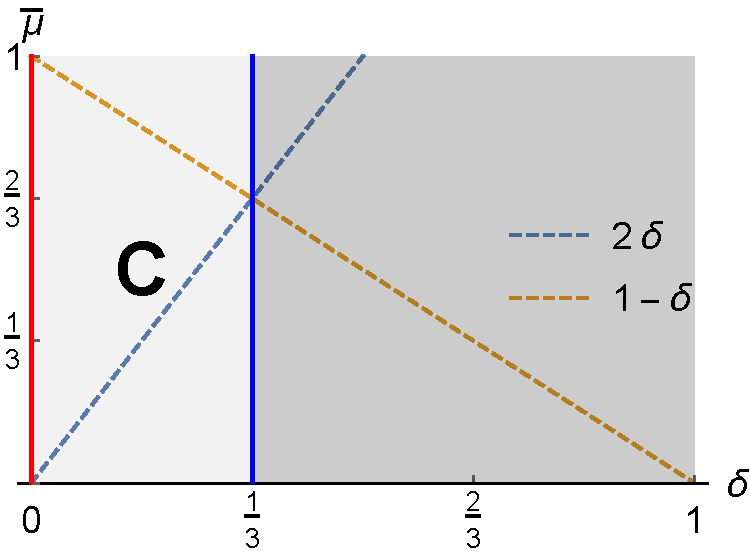
\includegraphics[scale=0.5]{prop_letter_ajhs_referee_response_nb}
\par\end{centering}
\caption{\label{fignoname}The region to the left of the vertical line at $\delta=\frac{1}{3}$
is where we assume small measurement degradation; in that region,
our extension of the KS theorem demonstrates contextuality (\textsf{C}).
In the region to the right, the degradation of the data is large,
and our extension of the KS theorem no longer refutes other explanations
for the experimental data.}
\end{figure}
The bound $\delta<\frac{1}{3}$ is tight as it is possible to construct
a $\frac{1}{3}$-deterministic QIVPM $\bar{\mu}\colon\events\rightarrow\mathscr{I}$.
For example, $\bar{\mu}_{2}'$ defined in Table~\ref{tab:probability-measures}
is a valid $\frac{1}{3}$-deterministic QIVPM\@. When $\delta\geq\frac{1}{3}$,
i.e., when the uncertainty in measurements becomes so large, it becomes
possible to map every observable to some (quite inaccurate) probability
interval, thus invalidating the Kochen-Specker theorem. We can summarize
and illustrate the above arguments using Fig.~\ref{fignoname}.

As is the case for conventional, infinitely-precise, quantum probability
measures, the theorem is only applicable to dimensions $D\geq3$.
Indeed, when the Hilbert space has dimension 2, it is straightforward
to construct a 0-deterministic QIVPM as follows. Consider a non-contextual
hidden variable model for $D=2$ (e.g., as proposed by Bell or Kochen-Specker~\cite{BELL_1966,kochenspecker1967}).
Such a two-dimensional model always assigns definite values to all
observables and hence assigns a \emph{determinate} probability (0
or 1) to each event. This probability measure directly induces a 0-deterministic
QIVPM by changing 0 to $\imposs$ and 1 to $\necess$. It follows
that every 0-deterministic QIVPM is $\delta$-deterministic.

\subsection{Experimental Data and $\delta$-determinism}

We have thus quantified one important aspect of uncertainty in quantum
mechanics—the effect of the imprecise nature of devices—which is a
novel addition to the theory of measurement. Indeed, as Heisenberg
emphasized in his famous microscope example~\cite{Heisenberg1983},
the conventional theory of measurement states that it is impossible
to precisely measure any property of a system without disturbing it
somewhat. Thus, there are fundamental limits to what one can measure
and these limits have traditionally been attributed to complementarity.
Our imprecision represents an \emph{additional} source of indeterminacy
beyond the inherent probabilistic nature of quantum mechanics.

In an experimental setup, $\delta$ is calculated as follows. To determine
the probability of any event, we typically repeat an experiment $m$
times and count the number of times we witness the event. This assumes
that for each run of the experiment we can determine, using our apparatus,
whether the event occurred or not. Assume an event has an ideal mathematical
probability of $0$, and we repeat the experiment $100$ times. In
a perfect world, we should be able to refute the event $100$ times
and calculate that the probability is $0$. We might also observe
the event $2$ times and refute it $98$ times and therefore calculate
the probability to be $0.02$. Note that this situation assumes perfect
measurement conditions and remains within the context of conventional
(real-valued) probability theory. The question we focus on is what
happens if we are only able to refute it $97$ times and are \emph{uncertain}
$3$ times? This is quite common in actual experiments. Mathematically
we can model this idea by stating that the probability of the event
is in the range $\left[0,0.03\right]$ which says that the probability
of the event could be $0$, $0.01$, $0.02$, or $0.03$ as each the
three uncertain records could either be evidence for the event or
against it. We just cannot nail it down given the current experimental
results and therefore represent the evidence as a ($\delta=$)$0.03$-deterministic
probability measure. The interesting observation is that the axioms
of probability theory (like additivity and convexity) impose enough
constraints on the structure of interval-valued quantum probability
measures to make them robust in the face of small non-vanishing $\delta$'s.

To see this idea in the context of a quantum experiment, consider
a three-dimensional Hilbert space with one-dimensional projectors~$P_{\rho}$,
two-dimensional projectors $P_{\rho}+P_{\sigma}$, and an experiment
that is repeated $12$ times. By the Kochen-Specker theorem, it is
impossible to build a probability measure that maps every projection
to either $0=\frac{0}{12}$ or $1=\frac{12}{12}$. That is, the assignment~$\bar{\mu}_{0}$
defined in Table~\ref{tab:probability-measures} is not a QIVPM\@.

Now consider what happens if $\frac{1}{4}$ of the data for \emph{every}
one-dimensional projector is uncertain. A potential account of this
degradation is to assign to each event $P$ the entire range of possibilities
$\bar{\mu}_{1}(P)$ as defined in Table~\ref{tab:probability-measures}.
This measure is not a valid QIVPM because it does not satisfy the
convexity condition: for any two orthogonal one-dimensional events
$P_{0}$ and $P_{1}$, the convexity condition requires $\bar{\mu}_{1}\left(P_{0}+P_{1}\right)\subseteq\bar{\mu}_{1}\left(P_{0}\right)+\bar{\mu}_{1}\left(P_{1}\right)$,
but $\bar{\mu}_{1}\left(P_{0}+P_{1}\right)=\left[\tfrac{3}{4},1\right]$
which is not a subset of $\left[0,\tfrac{1}{2}\right]=\bar{\mu}_{1}\left(P_{0}\right)+\bar{\mu}_{1}\left(P_{1}\right)$.
Interestingly, it is impossible to find any probability measure that
would be consistent with these observations, as the interval $\left[\tfrac{3}{4},1\right]$
is completely disjoint from the interval $\left[0,\tfrac{1}{2}\right]$
and no amount of shifting of assumptions regarding the precise outcome
of the uncertain observations could change that disjointness. However,
as shown next, a sharp transition occurs when $\delta=\tfrac{1}{3}$.

When the proportion of uncertain data reaches $\frac{1}{3}$, the
probability measure that assigns to each event the entire range of
possibilities is $\bar{\mu}_{2}$ defined in Table~\ref{tab:probability-measures}.
This is also not a valid probability measure by the same argument
as above. However, in this case, $\bar{\mu}_{2}\left(P_{0}+P_{1}\right)=\left[\tfrac{2}{3},1\right]$
and $\left[0,\tfrac{2}{3}\right]=\bar{\mu}_{2}\left(P_{0}\right)+\bar{\mu}_{2}\left(P_{1}\right)$
have a \emph{common point}. Hence, by assuming that the uncertain
data for one-dimensional projectors always support the associated
event, while those for two-dimensional projectors always refute the
event, we can find the probability measure~$\bar{\mu}_{2}'$ that
can be verified as a valid QIVPM and is consistent with the experimental
data.

A similar situation happens when more than $\frac{1}{3}$ of data
is uncertain. In particular, if half of the data is uncertain, the
probability measure~$\bar{\mu}_{3}$ that assigns to each event the
entire range of possibilities is already a QIVPM\@.

%%%%%%%%%%%%%%%%%%%%%%%%%%%%%%%%%%%%%%%%%%%%%%%%%%%%%%%%%%%%%%%%%%%


\section{The Born Rule and Gleason's Theorem\label{sec:Gleason}}

A conventional quantum probability measure can be easily constructed
from a state $\rho$ according to the Born rule \cite{Born1983,Mermin2007,Jaeger2007}.
According to Gleason's theorem~\cite{gleason1957,Redhead1987-REDINA,peres1995quantum},
this state $\rho$ is also the unique state consistent with any possible
probability measure.

\subsection{Finite-Precision Extension of Gleason's Theorem\label{subsec:Finite-Precision-Extension-of}}

In order to re-examine these results in our framework, we first reformulate
Gleason's theorem in QIVPMs using infinitely precise uncountable intervals~$\mathscr{I}_{\infty}=\set{\left[x,x\right]}{x\in\left[0,1\right]}$:

\begin{thm}[$\mathscr{I}_{\infty}$ Variant of the Gleason Theorem]\label{cor:Gleason's-1}In
a Hilbert space $\Hilb$ of dimension $D\geq3$, given a QIVPM~$\bar{\mu}\colon\events\rightarrow\mathscr{I}_{\infty}$,
the state $\rho$ consistent with~$\bar{\mu}$ on every projector
is unique, i.e., there exists a unique state~$\rho$ such that $\coreBorn\left(\bar{\mu},\events\right)=\{\rho\}$.
\end{thm}

Now let us consider relaxing $\mathscr{I}$ to a countable set of
finite-width intervals. As the intervals in the image of a QIVPM become
less and less sharp, we expect more and more states to be consistent
with it. In the limit of minimal sharpness, all states~$\rho$ are
consistent with the QIVPM 
\begin{equation}
\bar{\mu}\left(P\right)=\begin{cases}
\imposs & \textrm{ if }P=\mathbb{0}\,;\\
\necess & \textrm{ if }P=\mathbb{1}\,;\\
\unknown=\left[0,1\right] & \textrm{ otherwise}
\end{cases}
\end{equation}
mapping nearly all projections to the \emph{unknown} interval~\unknown.
There is however a subtlety: as we will show in Thm.~\ref{thm:Non-extensible-of-Gleason's}
later, it is possible for an arbitrary assignment of intervals to
projectors to be globally inconsistent, % \noindent For general QIVPMs mapping to imprecise intervals, we also
% want to seek a simple rule to construct them, and to understand which
% states are consistent with them. However, if measurement intervals are
% too imprecise, the state consistent with the results of measurements
% on some projectors might contradict the state induced by some other
% projectors. Indeed we can formally prove that, in general, there may
% be \emph{no} state consistent with some arbitrary QIVPM.
but before proving Thm.~\ref{thm:Non-extensible-of-Gleason's}, we
need the other two lemmas to simplify the proof of the convexity condition
again.

\begin{lemma}\label{thm:convex-3}Given a Hilbert space~$\Hilb$
of dimension~$3$, to verify $\bar{\mu}\colon\events\rightarrow\mathscr{I}$
is a QIVPM, it is sufficient to check Eqs.~(\ref{eq:QIVPM-constraints})
and 
\begin{equation}
\bar{\mu}\left(P'+P''\right)\subseteq\bar{\mu}\left(P'\right)+\bar{\mu}\left(P''\right)\label{amr-1}
\end{equation}
for each pair of orthogonal projectors $P'$ and~$P''$.\end{lemma}

\begin{proof}The most important part of the proof is to verify the
convexity condition for $\bar{\mu}$. Given a pair of commuting projectors
$P_{0}$ and $P_{1}$ on a three-dimensional Hilbert space, they can
be diagonalized by a common orthonormal basis $\Omega=\left\{ \ket{0},\ket{1},\ket{2}\right\} $.
Consider the function $\varphi\colon2^{\Omega}\rightarrow\events$
defined in Eq.~(\ref{eq:pullback-function}), there are two sets
of basis vectors $E_{0}$ and $E_{1}\subseteq\Omega$, such that $\varphi\left(E_{0}\right)=P_{0}$
and $\varphi\left(E_{1}\right)=P_{1}$. Since $E_{0}$ and $E_{1}$
are both subsets of a three-element set, their relation has only three
possibilities. The first possibility is that one of them is a subset
of the other one, $E_{0}\subseteq E_{1}$ or $E_{1}\subseteq E_{0}$.
The second possibility is that they are disjoint, $E_{0}\cap E_{1}=\emptyset$.
If neither of the previous possibilities is true, i.e., they have
some intersections, but no subset relation, then $E_{0}\cap E_{1}$,
$E_{0}\backslash E_{1}$, and $E_{1}\backslash E_{0}$ are all non-empty.
Together with the fact that $\Omega$ has only three elements, they
are all singleton sets. These three possibilities are going to be
discussed as follows.
\begin{itemize}
\item When one of them is a subset of the other one, say $E_{0}\subseteq E_{1}$,
we have $P_{0}P_{1}=\varphi\left(E_{0}\cap E_{1}\right)=P_{0}$ and
$P_{0}+P_{1}-P_{0}P_{1}=P_{1}$. Thus,
\begin{equation}
\bar{\mu}\left(P_{0}+P_{1}-P_{0}P_{1}\right)+\bar{\mu}\left(P_{0}P_{1}\right)=\bar{\mu}\left(P_{1}\right)+\bar{\mu}\left(P_{0}\right)\,.
\end{equation}
\item When $E_{0}\cap E_{1}=\emptyset$, we have $P_{0}P_{1}=\varphi\left(E_{0}\cap E_{1}\right)=\mathbb{0}$
and 
\begin{equation}
\bar{\mu}\left(P_{0}+P_{1}-P_{0}P_{1}\right)+\bar{\mu}\left(P_{0}P_{1}\right)=\bar{\mu}\left(P_{0}+P_{1}\right)\subseteq\bar{\mu}\left(P_{0}\right)+\bar{\mu}\left(P_{1}\right)\label{eq:QuantumInterval-valuedProbability-Inclusion-3}
\end{equation}
by Eq.~(\ref{amr-1}).
\item When $E_{0}\cap E_{1}$, $E_{0}\backslash E_{1}$, and $E_{1}\backslash E_{0}$
are all singleton sets, say $E_{0}\backslash E_{1}=\left\{ \ket{0}\right\} $,
$E_{1}\backslash E_{0}=\left\{ \ket{1}\right\} $, and $E_{0}\cap E_{1}=\left\{ \ket{2}\right\} $,
proving an equivalent condition for the convexity condition, Eq.~(\ref{eq:QuantumInterval-valuedProbability-Inclusion}),
is easier than proving Eq.~(\ref{eq:QuantumInterval-valuedProbability-Inclusion})
directly. Since one minus an interval maps this interval to its mirror
image, and reflection preserves the subset relations, the convexity
condition holds if and only if
\begin{equation}
\necess-\bar{\mu}\left(P_{0}P_{1}\right)+\necess-\bar{\mu}\left(P_{0}+P_{1}-P_{0}P_{1}\right)\subseteq\necess-\bar{\mu}\left(P_{0}\right)+\necess-\bar{\mu}\left(P_{1}\right)
\end{equation}
which is equivalent to
\begin{equation}
\bar{\mu}\left(\mathbb{1}-P_{0}P_{1}\right)+\bar{\mu}\left(\mathbb{1}-\left(P_{0}+P_{1}-P_{0}P_{1}\right)\right)\subseteq\bar{\mu}\left(\mathbb{1}-P_{0}\right)+\bar{\mu}\left(\mathbb{1}-P_{1}\right)
\end{equation}
because of Eq.~(\ref{eq:QIVPM-complement}). The last equation holds
because we can apply Eq.~(\ref{amr-1}) on the following chain of
equations:
\begin{equation}
\begin{aligned} & \bar{\mu}\left(\mathbb{1}-P_{0}P_{1}\right)+\bar{\mu}\left(\mathbb{1}-\left(P_{0}+P_{1}-P_{0}P_{1}\right)\right)=\bar{\mu}\left(\proj{0}+\proj{1}\right)+\bar{\mu}\left(\mathbb{0}\right)\\
\subseteq{} & \bar{\mu}\left(\proj{0}\right)+\bar{\mu}\left(\proj{1}\right)=\bar{\mu}\left(\mathbb{1}-P_{0}\right)+\bar{\mu}\left(\mathbb{1}-P_{1}\right)\,.
\end{aligned}
\end{equation}
\end{itemize}
Since the convexity condition holds for all three possibilities, $\bar{\mu}$
is a QIVPM.\end{proof}

\begin{lemma}\label{thm:convex-3-1}Given a Hilbert space~$\Hilb$
of dimension~$3$, to verify $\bar{\mu}\colon\events\rightarrow\mathscr{I}$
is a QIVPM, it is sufficient to check Eqs.~(\ref{eq:QIVPM-constraints})
and 
\begin{equation}
\bar{\mu}\left(\proj{\psi'}+\proj{\psi''}\right)\subseteq\bar{\mu}\left(\proj{\psi'}\right)+\bar{\mu}\left(\proj{\psi''}\right)\label{amr-3}
\end{equation}
for each pair of orthogonal states $\ket{\psi'}$ and $\ket{\psi''}$.\end{lemma}

\begin{proof}Since any projectors can be expressed as the sum of
orthogonal one-dimensional projectors, Eq.~(\ref{amr-3}) implies
Eq.~(\ref{amr-1}) by induction, and this lemma holds because of
Lemma~\ref{thm:convex-3}.\end{proof}

After we proved the lemmas, we can state and prove the theorem that
some assignment of intervals to projectors can be globally inconsistent.

\begin{thm}[Empty Cores Exist for General QIVPMs]\label{thm:Non-extensible-of-Gleason's}There
exists a Hilbert space $\Hilb$ and a QIVPM~$\bar{\mu}\colon\events\rightarrow\mathscr{I}$
such that $\coreBorn\left(\bar{\mu},\events\right)=\emptyset$.\end{thm}
%% ajh: fixed garbled statement, add $$

\begin{proof}To prove this theorem, we need to construct a QIVPM
on some Hilbert space and verify that there are no states that are
consistent (see Def.~\ref{def:Consistency}) with it on all possible
events. Assume a Hilbert space of dimension $D=3$ with orthonormal
basis $\left\{ \ket{0},\ket{1},\ket{2}\right\} $, let $\ket{\ps}=\frac{\ket{0}+\ket{1}}{\sqrt{2}}$,
$\ket{\ps'}=\frac{\ket{0}+\ket{2}}{\sqrt{2}}$, and assign 
\begin{equation}
\mathscr{I}_{0}=\left\{ \necess,\imposs,\unknown\right\} \,.\label{eq:3-value-intervals}
\end{equation}
Consider the map $\bar{\mu}\colon\events\rightarrow\mathscr{I}_{0}$
defined in Table~\ref{tab:non-Born-QIVPM}. We want to prove $\bar{\mu}$
is a QIVPM\@. Since it is easy to verify $\bar{\mu}$ satisfies Eqs.~(\ref{eq:QIVPM-constraints}),
it is sufficient by Lemma~\ref{thm:convex-3-1} to verify 
\begin{equation}
\bar{\mu}\left(\proj{\psi'}+\proj{\psi''}\right)\subseteq\bar{\mu}\left(\proj{\psi'}\right)+\bar{\mu}\left(\proj{\psi''}\right)\label{amr-2}
\end{equation}
for each pair of orthogonal states $\ket{\psi'}$ and $\ket{\psi''}$.
Since $\ket{0}$, $\ket{\ps}$, and $\ket{\ps'}$ are not orthogonal
to each other, at least one of $\bar{\mu}\left(\proj{\psi'}\right)$
and $\bar{\mu}\left(\proj{\psi''}\right)$ is unknown~$\unknown$,
which implies $\unknown\subseteq\bar{\mu}\left(\proj{\psi'}\right)+\bar{\mu}\left(\proj{\psi''}\right)$.
Together with the fact that every interval in $\mathscr{I}_{0}$ is
a subset of $\unknown$, Eq.~(\ref{amr-2}) holds, and $\bar{\mu}$
is a QIVPM\@.

\begin{table}
\begin{doublespace}
\noindent \centering{}\caption{\label{tab:non-Born-QIVPM}QIVPM~$\bar{\mu}\colon\events\rightarrow\mathscr{I}_{0}$
on a Hilbert space of dimension~$D=3$. Events are listed in the
column labeled by $P$.}
\begin{tabular}{cc}
\toprule 
$P$  & $\bar{\mu}\left(P\right)$\tabularnewline
\midrule
$\mathbb{0}$, $\proj{0}$, $\proj{\ps}$, $\proj{\ps'}$  & $\imposs$\tabularnewline
$\mathbb{1}$, $\mathbb{1}-\proj{0}$, $\mathbb{1}-\proj{\ps}$, $\mathbb{1}-\proj{\ps'}$  & $\necess$\tabularnewline
All other projectors  & $\unknown$\tabularnewline
\bottomrule
\end{tabular}
\end{doublespace}
\end{table}
Next, we will prove by contradiction that $\coreBorn\left(\bar{\mu},\events\right)$
is the empty set. Suppose there is a state $\rho=\sum_{j=1}^{N}q_{j}\proj{\phi_{j}}\in\coreBorn\left(\bar{\mu},\events\right)$,
where $\sum_{j=1}^{N}q_{j}=1$ and $q_{j}>0$. Since we assumed the
core $\coreBorn\left(\bar{\mu},\events\right)$ is non-empty, so $\muB_{\rho}(P)\in\bar{\mu}(P)$,
and Table~\ref{tab:non-Born-QIVPM} tells us that $\bar{\mu}(\proj{0})=\imposs=[0,0]$,
we must conclude that $\muB_{\rho}(\proj{0})=0\in[0,0]$, and similarly
for $\proj{\ps}$ and $\proj{\ps'}$. If this is true, then $\ip{0}{\phi_{j}}=\ip{\ps}{\phi_{j}}=\ip{\ps'}{\phi_{j}}=0$
for all~$j$, and thus 
\begin{align}
\ip{1}{\phi_{j}}=\sqrt{2}\ip{\ps}{\phi_{j}}-\ip{0}{\phi_{j}}=0\,, &  & \ip{2}{\phi_{j}}=\sqrt{2}\ip{\ps'}{\phi_{j}}-\ip{0}{\phi_{j}}=0\,.
\end{align}
The above equations imply $\ket{\phi_{j}}=\ket{0}\ip{0}{\phi_{j}}+\ket{1}\ip{1}{\phi_{j}}+\ket{2}\ip{2}{\phi_{j}}=0$,
violating the assumption that $\ket{\phi_{j}}$ is a normalized state,
and thus the theorem is proved.\end{proof}

The fact that a collection of poor measurements on a quantum system
cannot reveal the underlying state is not surprising. Under certain
conditions, we can however guarantee that the uncertainty in measurements
is consistent with \emph{some} non-empty collection of quantum states.
Furthermore, we can relate the uncertainty in measurements to the
volume of quantum states such that, in the limit of infinitely precise
measurements, the volume of states collapses to a single state.

To that end, we introduce the concept of \emph{interval maps}, which
we can use to construct a consistent family of QIVPMs. An interval
map $f\colon\left[0,1\right]\rightarrow\mathscr{I}$ maps every real-valued
probability $x\in\left[0,1\right]$ to a set of intervals $f\left(x\right)=\left[\ell,r\right]$
containing $x$, where $\left[0,1\right]$ denotes the set of real-valued
probabilities (this should not be confused with the interval-valued
probability $\unknown$). We also need a notion of \emph{norm} to
quantify the uncertainty in measurements and the distance between
(pure or mixed) states. The norm of a collection of intervals $\mathscr{I}$,
$\left\Vert \mathscr{I}\right\Vert $, is defined as the maximum length
of intervals in it. The norm of a pure state $\rho=\proj{\psi}$ is
defined as usual by $\left\Vert \psi\right\Vert =\sqrt{\ip{\psi}{\psi}}$.
For any given Hermitian operator~$A$, we choose the operator norm
$\left\Vert A\right\Vert =\max_{\left\Vert \psi\right\Vert =1}\left\Vert A\ket{\psi}\right\Vert $,
which is also known as the $2$-norm or the spectral norm~\cite{RobertsVarberg1973,peres1995quantum,GolubVanLoan1996,Foucart2012}.
In fact, for any such matrix, including the density matrix~$\rho$,
this norm is the maximum absolute value of its eigenvalues. Then,
a finite-precision extension of Gleason's theorem can be stated as
follows.

\begin{thm}[Finite-Precision Extension of the Gleason Theorem]\label{thm:Finite-precision-Gleason}Let
$f\colon\left[0,1\right]\rightarrow\mathscr{I}$ be an interval map
and let the composition $f\circ\muB_{\rho}$ be a QIVPM, where $\muB_{\rho}$
is the probability measure induced by the Born rule for a given state~$\rho$.
If a state $\rho'$ is consistent with $f\circ\muB_{\rho}$ on all
events, i.e., $\rho'\in\coreBorn\left(f\circ\muB_{\rho},\events\right)$,
then the norm of their difference is bounded by $\left\Vert \mathscr{I}\right\Vert $,
i.e., $\left\Vert \rho-\rho'\right\Vert \le\left\Vert \mathscr{I}\right\Vert $.\end{thm}

\begin{proof}Given a state~$\rho'$ consistent with $f\circ\muB_{\rho}$,
we have $\muB_{\rho'}\left(\proj{\psi}\right)\in f\left(\muB_{\rho}\left(\proj{\psi}\right)\right)$
for any one-dimensional projector $P=\proj{\psi}$. Since the maximum
length of the intervals in $\mathscr{I}$ is $\left\Vert \mathscr{I}\right\Vert $,
it is also the upper bound of the difference: 
\begin{equation}
\left|\muB_{\rho'}\left(\proj{\psi}\right)-\muB_{\rho}\left(\proj{\psi}\right)\right|=\left|\melem{\psi}{\rho-\rho'}{\psi}\right|\le\left\Vert \mathscr{I}\right\Vert \,.
\end{equation}
Since $\rho-\rho'$ is Hermitian, $\max_{\left\Vert \psi\right\Vert =1}\left|\melem{\psi}{\rho-\rho'}{\psi}\right|$
is the maximum absolute value of the eigenvalues of $\rho-\rho'$~\cite{544199},
and equal to $\left\Vert \rho-\rho'\right\Vert $~\cite{GolubVanLoan1996,Foucart2012}.
Hence, $\left\Vert \rho-\rho'\right\Vert \le\left\Vert \mathscr{I}\right\Vert $.\end{proof}

\subsection{Ultramodular Functions\label{subsec:Ultramodular-Functions}}

Theorem~\ref{thm:Finite-precision-Gleason} generalizes Gleason's
theorem in the sense that it accounts for a larger class of probability
measures that includes the conventional one as a limit. The theorem
is however ``special'' in the sense that it only applies to the
particular class of QIVPMs constructed by composing an interval map
with a conventional quantum probability measure. QIVPMs constructed
in this manner have some peculiar properties that we examine next.

An interval map is called \emph{ultramodular} if it satisfies the
following properties.

\begin{definition}[Ultramodular Functions]\label{def:THOS}Given
a collection of intervals $\mathscr{I}$ including $\imposs$ and
$\necess$, an interval map $\ultramodular\colon\left[0,1\right]\rightarrow\mathscr{I}$
is called ultramodular if
\begin{align}
\ultramodular(0)=\imposs\,, &  & \ultramodular(1)=\necess\,, &  & \ultramodular\left(1-x\right)=\necess-\ultramodular\left(x\right)\,,\label{eq:iota-constraints}
\end{align}
and for any three numbers~$x_{0}$, $x_{1}$, and $x_{2}\in\left[0,1\right]$
such that $y=x_{0}+x_{1}+x_{2}\in\left[0,1\right]$, we have
\begin{equation}
\ultramodular\left(y\right)+\ultramodular\left(x_{2}\right)\subseteq\ultramodular\left(x_{0}+x_{2}\right)+\ultramodular\left(x_{1}+x_{2}\right)\,.\label{eq:iota-Inclusion}
\end{equation}
\end{definition}

\noindent The first three constraints, Eqs.~(\ref{eq:iota-constraints}),
are the direct counterpart of the corresponding QIVPM constraints,
Eqs.~(\ref{eq:QIVPM-constraints}); the last condition, Eq.~(\ref{eq:iota-Inclusion}),
is the direct counterpart of the convexity conditions, Eqs.~(\ref{eq:classicalconvex})
and~(\ref{eq:QuantumInterval-valuedProbability-Inclusion}) \cite{Choquet1954,Shapley1971,NgMoYeh1997Chinese,MarinacciMontrucchio2005}.
Therefore, these conditions guarantee that for any conventional quantum
probability measure $\mu$, the composition $\ultramodular\circ\mu$
defines a valid QIVPM\@. Conversely, if for every quantum probability
measure $\mu$, it is the case that $f\circ\mu$ is a QIVPM, then
the interval map~$f$ is an ultramodular function. Formally, we have
the following result:

\begin{thm}[Equivalence of Ultramodular Functions and IVPMs]\label{thm:iota-statements}The
following three statements are equivalent: \begin{enumerate}

\item\label{enu:iota-subject-to}A function~$\ultramodular\colon\left[0,1\right]\rightarrow\mathscr{I}$
is ultramodular.

\item\label{enu:iota-mu-CIVPM}The composite function $\ultramodular\circ\mu\colon2^{\Omega}\rightarrow\mathscr{I}$
is a classical IVPM for all classical probability measures $\mu\colon2^{\Omega}\rightarrow\left[0,1\right]$.

\item\label{enu:iota-mu-QIVPM}The composite function $\ultramodular\circ\mu\colon\events\rightarrow\mathscr{I}$
is a QIVPM for all quantum probability measures $\mu\colon\events\rightarrow\left[0,1\right]$.
\end{enumerate} \end{thm}

\begin{proof}Statement~\ref{enu:iota-subject-to} implies~\ref{enu:iota-mu-CIVPM}
and~\ref{enu:iota-mu-QIVPM} as we have outlined above. Conversely,
for the quantum case, we want to show that if $\ultramodular$ is
not ultramodular, then for some quantum probability measure $\mu$,
the composite $\ultramodular\circ\mu$ might not be a QIVPM\@. Suppose
there are three particular numbers~$x_{0}$, $x_{1}$, and $x_{2}\in\left[0,1\right]$
such that $y=x_{0}+x_{1}+x_{2}\in\left[0,1\right]$, but they don't
satisfy Eq.~(\ref{eq:iota-Inclusion}). Consider the state: 
\begin{equation}
\rho=x_{0}\proj{0}+x_{1}\proj{1}+x_{2}\proj{2}+\left(1-y\right)\proj{3}\,.
\end{equation}
The induced map $\ultramodular\circ\muB_{\rho}$ constructed using
the Born rule and blurred by $\ultramodular$ fails to satisfy Eq.~(\ref{eq:QuantumInterval-valuedProbability-Inclusion})
when $P_{0}=\proj{0}+\proj{2}$ and $P_{1}=\proj{1}+\proj{2}$. In
other words, this induced map fails to be a QIVPM\@.

For the classical case, if $\ultramodular$ is not ultramodular, we
also want to find a classical probability measure $\mu\colon2^{\Omega}\rightarrow\left[0,1\right]$
such that $\ultramodular\circ\mu$ is not a classical IVPM\@. Consider
an orthonormal basis $\Omega=\{\ket{0},\ket{1},\ldots,\ket{D-1}\}$
and $\varphi\colon2^{\Omega}\rightarrow\events$ defined by Eq.~(\ref{eq:pullback-function}).
Notice that the pullback of our previous quantum probability measure
$\muB_{\rho}$, $\varphi^{*}\muB_{\rho}$, is a classical probability
measure. If we pick $\mu$ as $\varphi^{*}\muB_{\rho}$, then the
induced map $\ultramodular\circ\mu$ fails to be a classical IVPM
for the same reason as in the quantum case.\end{proof}

In other words, the essential properties of QIVPMs constructed using
interval maps can be gleaned from the properties of ultramodular functions.
The following is the most interesting property in our setting.

\begin{thm}[Range of Ultramodular Functions]\label{thm:convex-uncountable}For
any ultramodular function~$\ultramodular\colon\left[0,1\right]\rightarrow\mathscr{I}$,
either $\mathscr{I}=\mathscr{I}_{0}$ as defined in Eq.~(\ref{eq:3-value-intervals})
or $\mathscr{I}$ contains uncountably many intervals.\end{thm}

\begin{proof}Since $\ultramodular$ maps to intervals, we can decompose
it into two functions: its left-end and right-end, where $\left[\ultramodularL\left(x\right),\ultramodularR\left(x\right)\right]=\ultramodular\left(x\right)$.
By Eq.~(\ref{eq:iota-Inclusion}), the left-end function $\ultramodularL\colon\left[0,1\right]\rightarrow\left[0,1\right]$
is Wright-convex~\cite{Wright1954,RobertsVarberg1973,PecaricTong1992},
i.e., 
\begin{equation}
\ultramodularL\left(y\right)+\ultramodularL\left(x_{2}\right)\ge\ultramodularL\left(x_{0}+x_{2}\right)+\ultramodularL\left(x_{1}+x_{2}\right)
\end{equation}
for three numbers~$x_{0}$, $x_{1}$, and $x_{2}\in\left[0,1\right]$
with $y=x_{0}+x_{1}+x_{2}\in\left[0,1\right]$. Together with the
fact that $\ultramodularL$ maps to a bounded interval $\left[0,1\right]$,
the left-end function~$\ultramodularL$ must be continuous on the
unit open interval $\left(0,1\right)$~\cite{MarinacciMontrucchio2005}.
Therefore, either $\ultramodular$ maps every number in $\left(0,1\right)$
to the same interval, or the number of intervals to which $\ultramodular$
maps must be uncountable.\end{proof}

To summarize, a conventional quantum probability measure has an uncountable
range $[0,1]$. A QIVPM constructed by blurring such a conventional
quantum probability measure must also have an uncountable range of
intervals. Of course, any particular QIVPM, or any particular experiment,
will use a fixed collection of intervals appropriate for the resources
and precision of the particular experiment.

\chapter{Conclusion and Further Discussion\label{chap:Further-Discussion}}

\section{Summary}

Conventional quantum theory is based on the continuum of complex numbers,
but we cannot distinguish two arbitrary complex numbers without unbounded
resources. To explore alternative versions of quantum theory incorporating
our limitation of distinguishability, two types of discrete quantum
theories were described: \emph{quantum theories and computing over
finite fields} and \emph{quantum interval-valued probability measures
(QIVPMs)}. Examining the computational and physical consequences of
such frameworks can yield new insights into not only the subtle properties
of conventional quantum theory but also the power and capacity of
quantum computing.

The theories over finite fields started with unrestricted discrete
fields (Chapter~\ref{chap:Unrestricted-Finite-Fields}), then advanced
to a more reasonable framework based on complexifiable discrete fields
(Secs.~\ref{discretequantumtheoryI} to~\ref{discretequantumcomputingI}),
which lacks a notion of probability and supports unnaturally efficient
deterministic quantum algorithms. A still more plausible discrete
theory with cardinal probabilities was proposed (Secs.~\ref{sec:Discrete-Quantum-Theory-(II)}
and~\ref{discretequantumcomputingII}), where conventional quantum
theory and computing emerge in a local sense, but lacking arithmetic
operations among cardinal probabilities still posed difficulty to
define expectation values. Since the axiomatic approach looked unlikely
to provide sensible real-valued probability measures over finite fields
(Sec.~\ref{sec:Toward-IVPM}), we shifted our attention to directly
embed our limitation of distinguishability into the theory to define
QIVPM.

\begin{figure}[b]
\centering{}$\xymatrix{\textrm{Classical Probability Measure}\ar[d]_{\textrm{blur probability}}\ar[rr]^{\textrm{glue events}} &  & \textrm{Quantum Probability Measure}\ar[d]^{\textrm{blur probability}}\\
\textrm{Classical IVPM}\ar[rr]_{\textrm{glue events}} &  & \textrm{QIVPM}
}
$\caption{\label{fig:commutative-diagrams}QIVPMs inherit from both quantum
probability measures and classical IVPMs.}
\end{figure}
As a natural extension of both conventional quantum probability measures
and classical interval-valued probability measures (IVPMs) illustrated
in Fig.~\ref{fig:commutative-diagrams}, QIVPMs inherit definitions
and properties from the both sides. While the expectation values of
QIVPMs can be pulled back to the classical cases and consistent with
those of quantum probability measures in the infinitely precise limit
(Sec.~\ref{sec:Interval-Uncertainty}), foundational concepts in
quantum mechanics, such as the Kochen-Specker and Gleason theorems,
extended to QIVPMs in subtle ways. By carefully specifying experimental
uncertainties, we established rigorous bounds on the validity of the
Kochen-Specker theorem (Sec.~\ref{sec:Kochen-Specker}). While there
is a QIVPM not consistent with Gleason's unique state~$\rho$ on
all projectors, we constructed a class of QIVPMs for which the original
Gleason theorem could be recovered asymptotically (Sec.~\ref{sec:Gleason}).

In the following further discussion, we will briefly explain why we
only recovered Gleason's on a class of QIVPMs, the possibility to
further build a computational model over QIVPMs, and the possibility
combining both approaches to consider quantum interval-valued probability
measures over finite fields.

\section{Gleason's Theorem for General QIVPMs}

\begin{comment}
When people proved the original Gleason theorem, people usually exploited
the geometrical structure of real 3-dimensional Hilbert space \cite{gleason1957,peres1995quantum,RichmanBridges1999,Hamhalter2013}.
Since our finite-precision extension of the Gleason theorem only applies
on a class of QIVPMs, we might want to ask how to modify these geometrical
arguments to have a Gleason-type theorem for general QIVPMs. We will
further study the tensor product structure among QIVPMs which is essential
for defining product and entangled states and serves the basis to
discuss quantum nonlocality~\cite{Bell1964,Redhead1987-REDINA,peres1995quantum,Jaeger2007}
and quantum computing with QIVPMs. Finally, we want to improve the
discrete quantum theories to consider QIVPMs over finite fields in
future research.
\end{comment}
As we discussed in Sec.~\ref{sec:Gleason}, Thm.~\ref{thm:Finite-precision-Gleason}
only applies to the QIVPMs constructed by composing an interval map
with a conventional quantum probability measure, and the states consistent
with the composite QIVPM collapse to a single state as the maximum
length of intervals in $\mathscr{I}$, $\left\Vert \mathscr{I}\right\Vert $,
shrinks to $0$. In contrast, the globally inconsistent QIVPM defined
in Table~\ref{tab:non-Born-QIVPM} has the least sharp range~$\mathscr{I}_{0}$
with $\left\Vert \mathscr{I}_{0}\right\Vert =1$. This suggests a
possibility that shrinking the length $\left\Vert \mathscr{I}\right\Vert $
might help to regularize general QIVPMs, and it is natural to ask
whether there is a short enough length~$\varepsilon$ such that QIVPMs
mapping to intervals not longer than $\varepsilon$ always have non-empty
cores.

\begin{question}\label{question:approximation-Gleason}Given a Hilbert
space $\Hilb$ of dimension $D\geq3$, is there an $\varepsilon>0$
such that for all QIVPM $\bar{\mu}\colon\events\rightarrow\mathscr{I}$
satisfying $\left\Vert \mathscr{I}\right\Vert \le\varepsilon$, $\bar{\mu}$
must have a non-empty core, i.e., $\coreBorn\left(\bar{\mu},\events\right)\ne\emptyset$
?\end{question}

\begin{comment}

\chapter{Conclusion\label{chap:Conclusion}}

\todo{Add a two-page conclusion chapter which could include further
discussion, but it can be only a few sentences? }\todo{Discrete
\textgerman[variant=german,spelling=new,babelshorthands=true]{Schrödinger}
equation? And its relationship with Grover's algorithm? }\todo{Notice
that in differential geometry, the Killing-Hopf theorem asserts that
having positive constant curvature guarantees a manifold is essentially
a sphere, but say little things even if the curvature has an only
small deviation from constant. Since a quantum probability measure
is glued by classical probability measures, like a manifold. When
their relations are exact, Gleason's theorem asserts that a quantum
probability measure can be essentially induced by the Born rule, but
they can be wild when we move on to the interval-valued situation!
}
\end{comment}
To better understand this question, consider the $D=3$ situation,
where any two-dimensional projectors can be expressed as the complement
of a one-dimensional projector, and by Eq.~(\ref{eq:QIVPM-complement})
so does their interval-valued probabilities, i.e., 
\begin{equation}
\bar{\mu}\left(\mathbb{1}-\proj{\psi}\right)=\necess-\bar{\mu}\left(\proj{\psi}\right)\,.\label{eq:QIVPM-complement-states}
\end{equation}
Hence, a QIVPM is completely determined by its values on the one-dimensional
projectors which are one-to-one corresponding to the irreducible states,
and these irreducible states are encoded in the complex projective
space $\CP{2}$ as we discussed in Sec.~\ref{subsec:Explicit-generalization-of}.
Therefore, to study a QIVPM~$\bar{\mu}$, we can just study a pair
of functions $\frameL\colon\CP{2}\rightarrow\left[0,1\right]$ and
$\frameR\colon\CP{2}\rightarrow\left[0,1\right]$ defined by $[\frameL\left(\ket{\psi}\right),\frameR\left(\ket{\psi}\right)]=\bar{\mu}\left(\proj{\psi}\right)$
for any irreducible state $\ket{\psi}\in\CP{2}$. According to Lemma~\ref{thm:convex-3-1},
$\bar{\mu}\colon\events\rightarrow\mathscr{I}$ is a QIVPM if and
only if $\bar{\mu}$ satisfies Eqs.~(\ref{eq:QIVPM-constraints})
and
\begin{equation}
\bar{\mu}\left(\mathbb{1}-\proj{\psi_{0}}\right)\subseteq\bar{\mu}\left(\proj{\psi_{1}}\right)+\bar{\mu}\left(\proj{\psi_{2}}\right)\label{eq:interval-valued-inclusion}
\end{equation}
for all orthonormal basis $\left\{ \ket{\psi_{i}}\right\} _{i=0}^{2}$
because $\proj{\psi_{1}}+\proj{\psi_{2}}=\mathbb{1}-\proj{\psi_{0}}$.
By applying Eq.~(\ref{eq:QIVPM-complement-states}) on the left-hand
side, Eq.~(\ref{eq:interval-valued-inclusion}) is equivalent to
the following interval-inclusion
\begin{eqnarray}
 &  & \necess-\left[\frameL\left(\ket{\psi_{0}}\right),\frameR\left(\ket{\psi_{0}}\right)\right]\subseteq\left[\frameL\left(\ket{\psi_{1}}\right),\frameR\left(\ket{\psi_{1}}\right)\right]+\left[\frameL\left(\ket{\psi_{2}}\right),\frameR\left(\ket{\psi_{2}}\right)\right]\label{eq:interval-valued-frame-function}\\
 & \Leftrightarrow & \left[1-\frameR\left(\ket{\psi_{0}}\right),1-\frameL\left(\ket{\psi_{0}}\right)\right]\subseteq\left[\frameL\left(\ket{\psi_{1}}\right)+\frameL\left(\ket{\psi_{2}}\right),\frameR\left(\ket{\psi_{1}}\right)+\frameR\left(\ket{\psi_{2}}\right)\right]\,.\nonumber 
\end{eqnarray}
This interval-inclusion can be rephrased as a long inequality
\begin{equation}
\frameL\left(\ket{\psi_{1}}\right)+\frameL\left(\ket{\psi_{2}}\right)\le1-\frameR\left(\ket{\psi_{0}}\right)\le1-\frameL\left(\ket{\psi_{0}}\right)\le\frameR\left(\ket{\psi_{1}}\right)+\frameR\left(\ket{\psi_{2}}\right)\,.
\end{equation}
Since $\left\Vert \mathscr{I}\right\Vert \le\varepsilon$, the length
of every interval $\left[\frameL\left(\ket{\psi}\right),\frameR\left(\ket{\psi}\right)\right]$
is bounded by $\varepsilon$ as well, which implies the largest term
in the previous inequality $\frameR\left(\ket{\psi_{1}}\right)+\frameR\left(\ket{\psi_{2}}\right)$
is bounded by $\frameL\left(\ket{\psi_{1}}\right)+\frameL\left(\ket{\psi_{2}}\right)+2\varepsilon$.
In other words, the left-end function~$\frameL$ satisfies the following
inequalities
\begin{subequations}
\begin{eqnarray}
 &  & \frameL\left(\ket{\psi_{1}}\right)+\frameL\left(\ket{\psi_{2}}\right)\le1-\frameL\left(\ket{\psi_{0}}\right)\le\frameL\left(\ket{\psi_{1}}\right)+\frameL\left(\ket{\psi_{2}}\right)+2\varepsilon\\
 & \Leftrightarrow & 1-2\varepsilon\le\sum_{i=0}^{2}\frameL\left(\ket{\psi_{i}}\right)\le1\,.\label{eq:left-end-frame-function}
\end{eqnarray}
\end{subequations}
In this language, Gleason's theorem basically states that when $\varepsilon=0$,
given any function $\frameL\colon\CP{2}\rightarrow\left[0,1\right]$
satisfying Eq.~(\ref{eq:left-end-frame-function}), there exists
a unique mixed state~$\rho$ such that 
\begin{equation}
\frameL\left(\ket{\psi}\right)=\melem{\psi}{\rho}{\psi}\label{eq:Gleason-for-CP2}
\end{equation}
for any state $\ket{\psi}\in\CP{2}$. Our Question~\ref{question:approximation-Gleason}
then ask how $\frameL$ would look like with a positive $\varepsilon$.

With different settings, whether there is an approximate version of
Gleason's theorem was asked by Sam Sanders in \emph{constructivenews}
on 2013~\cite{Sanders2013}, and there is no clear answer for his
question. To have an idea of how hard this question could be, recall
in Sec.~\ref{sec:fuzzy} we state that a quantum probability space
is glued by a family of classical probability spaces. This is like
the situation that a manifold is glued by many local coordinates.
When each small piece has \emph{exactly} the same and positive curvature,
the Killing-Hopf theorem asserts this manifold is a sphere, but little
can we say even if the curvature has a small deviation from constant.
A similar situation might happen when approximating Gleason's theorem,
but this time the whole space is glued by ``local'' classical probability
space defined by each orthonormal basis $\left\{ \ket{\psi_{i}}\right\} _{i=0}^{2}$.
When the sum of $\frameL$, $\sum_{i=0}^{2}\frameL\left(\ket{\psi_{i}}\right)$,
is \emph{exactly} the same and equal to $1$, Gleason's theorem asserts
that $\frameL$ can be expressed as Eq.~(\ref{eq:Gleason-for-CP2}).
However, when each local classical probability space becomes imprecise,
a general $\frameL$ might be as wild as we can imagine, and we might
need to know a bit more, like its QIVPM is a composite function, to
deduce its global property.

\section{And Beyond\ldots}

After we build the quantum interval-valued probability model, we might
want to know how powerful a quantum computer could be based on this
model. Since the conventional quantum circuit model manipulates the
probability amplitudes instead of the measured probabilities, either
a quantum computing model above QIVPMs needs to simultaneously manipulate
all states in the core of a QIVPM, or we need to find a way to manipulate
a QIVPM directly. However, both strategies are not straightforward.
On one hand, as we proved in Thm.~\ref{thm:Non-extensible-of-Gleason's},
a QIVPM might have an empty core which cannot be evolved over time.
On the other hand, if we want to manipulate and compute QIVPMs directly
for multi-qubit algorithms, we need to glue the QIVPM for each qubit
or subsystem together to get the QIVPM of the whole system, and this
is not straightforward either.

A successful interval-valued theory might be further extended over
finite fields based on the following definition.

\begin{definition}[Quantum Interval-valued Probability Measures
over Finite Fields]\label{def:QIVPMFF}Consider a vector space~$\mathcal{H}$
of dimension~$D$ over the complexified field~$\Fpp$, its set of
events~$\events_{p^{2}}$ as defined in Def.~\ref{def:QPMFF}, and
a collection of intervals~$\mathscr{I}$. A quantum interval-valued
probability measure over finite field $\bar{\mu}\colon\events_{p^{2}}\rightarrow\mathscr{I}$
assigns an interval to each event~$P$ subject to $\bar{\mu}(\mathbb{0})=\imposs$,
$\bar{\mu}(\mathbb{1})=\necess$, $\bar{\mu}\left(\mathbb{1}-P\right)=\necess-\bar{\mu}\left(P\right)$,
and satisfying for each pair of \emph{commuting} events~$P_{0}$
and~$P_{1}$ with $P_{0}P_{1}=P_{1}P_{0}$, 
\begin{equation}
\bar{\mu}\left(P_{0}+P_{1}-P_{0}P_{1}\right)+\bar{\mu}\left(P_{0}P_{1}\right)\subseteq\bar{\mu}\left(P_{0}\right)+\bar{\mu}\left(P_{1}\right)\,.\label{eq:QuantumInterval-valuedProbability-Inclusion-Finite-Field}
\end{equation}
\end{definition}

\noindent Understanding the properties of these probability measures
and whether we could define a ``sensible'' Born rule upon them combines
two approaches for dealing with the continuous quantities used in
the conventional quantum theory and will be the next natural extension
for our discrete quantum theories and computing.


\clearpageAddContents{chapter}{Bibliography} %
\begin{comment}
\printbibliography
\end{comment}
\printbibliography

\addContentsChapterWithoutPagenumber{Curriculum Vitae}

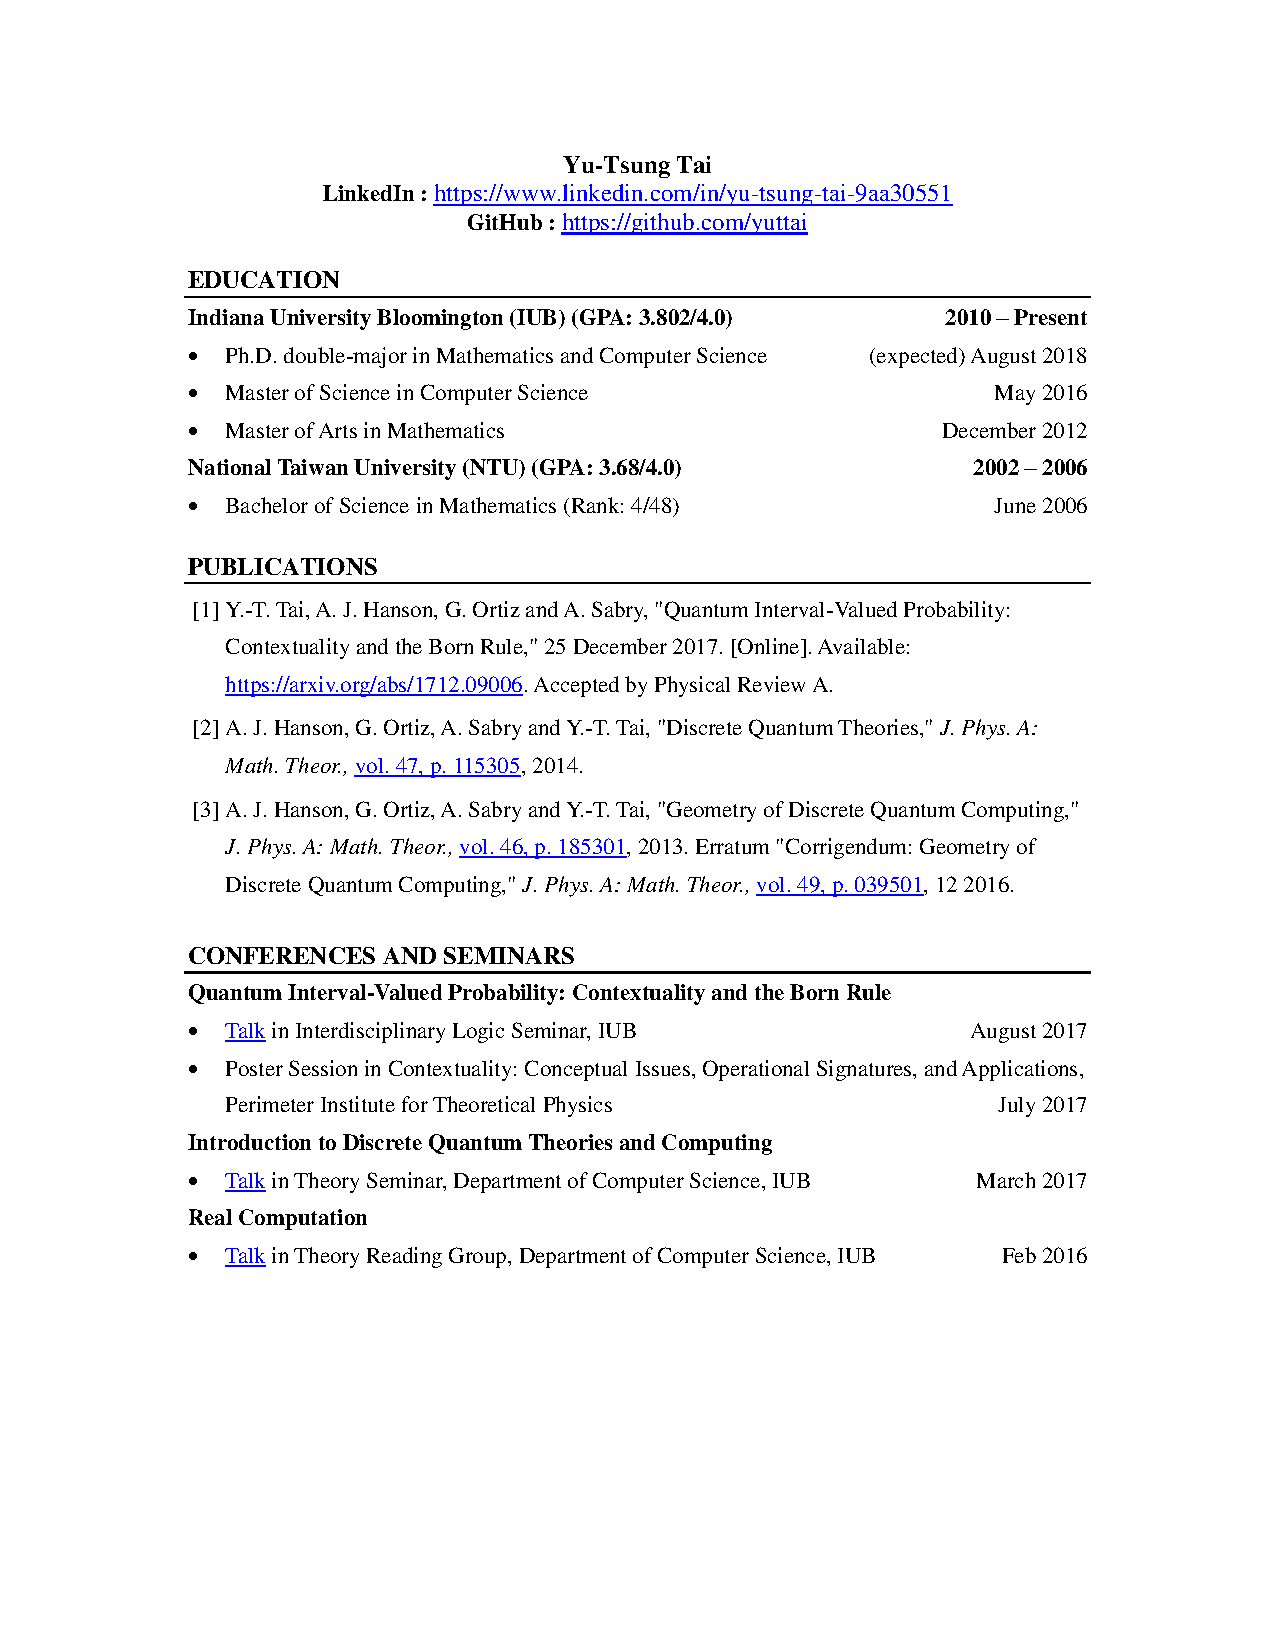
\includepdf[pages=-]{CV_thesis}
\end{document}
